\newcommand*{\TeXturedVERSION}{1.5.0} %% TeXtured 2025-08-06
%%%%%%%%%%%%%%%%%%%%%%%%%%%%%%%%%%%%%%%%%%%%%%%%%%%%%%%%%%%%%%%%%%%%%%%
%% NOTE: If you find any issues or have any suggestions, please open %%
%%       an Issue on GitHub: https://github.com/jdujava/TeXtured     %%
%%%%%%%%%%%%%%%%%%%%%%%%%%%%%%%%%%%%%%%%%%%%%%%%%%%%%%%%%%%%%%%%%%%%%%%

%% Enable built-in LaTeX support for PDF/A compliance (must be before `\documentclass`)
\DocumentMetadata{lang=en, pdfversion=1.7, pdfstandard=A-2u}
%%% PDF/A compliance - glyph to Unicode mappings

%% NOTE: metadata are set up using the `hyperref` package in `preamble/general/hyperref.tex`

%% WARN: `pdfx` package is SUPERSEDED by built-in LaTeX support for PDF/A
%%       However, in case additional fonts are used, some glyphs may not be covered
%%       by default Unicode mappings, in which case they need to be mapped to Unicode
%%       code points manually (see below for GUIDE and examples).

%%% GUIDE: How to add missing unicode mappings for glyphs
%%
%% Consider following part of VeraPDF output for a non-compliant PDF:
%%   <rule specification="ISO 19005-2:2011" clause="6.2.11.7.2" testNumber="1" status="failed" passedChecks="0" failedChecks="1">
%%     <description>The Font dictionary of all fonts shall define the map of all used character codes to Unicode values,
%%                  either via a ToUnicode entry, or other mechanisms as defined in ISO 19005-2, 6.2.11.7.2.</description>
%%     <object>Glyph</object>
%%     <test>toUnicode != null</test>
%%     <check status="failed">
%%       <context>root/document[0]/pages[58](1323 0 obj PDPage)/contentStream[0](1324 0 obj PDContentStream)
%%                                          /operators[654]/usedGlyphs[0](RMTQUN+MSAM10 RMTQUN+MSAM10 57 0  0)</context>
%%       <errorMessage>The glyph can not be mapped to Unicode</errorMessage>
%%     </check>
%%   </rule>
%%
%% This means that some glyph on page 59 (indicated by a 0-based index `pages[58]`)
%% is missing a Unicode mapping. To fix this, we need to find the name of the glyph,
%% and provide a Unicode mapping for it. For further instructions how to proceed see
%% `preamble/pdfA-compliance/LaTeX-find-glyph-name/LaTeX-find-glyph-name.tex`.

\RequirePackage{iftex}
\ifluatex % only for luaLaTeX (sourced by default for pdfLaTeX)
    \RequirePackage{luatex85}
    %%% PDF/A compliance - glyph to Unicode mappings

%% NOTE: metadata are set up using the `hyperref` package in `preamble/general/hyperref.tex`

%% WARN: `pdfx` package is SUPERSEDED by built-in LaTeX support for PDF/A
%%       However, in case additional fonts are used, some glyphs may not be covered
%%       by default Unicode mappings, in which case they need to be mapped to Unicode
%%       code points manually (see below for GUIDE and examples).

%%% GUIDE: How to add missing unicode mappings for glyphs
%%
%% Consider following part of VeraPDF output for a non-compliant PDF:
%%   <rule specification="ISO 19005-2:2011" clause="6.2.11.7.2" testNumber="1" status="failed" passedChecks="0" failedChecks="1">
%%     <description>The Font dictionary of all fonts shall define the map of all used character codes to Unicode values,
%%                  either via a ToUnicode entry, or other mechanisms as defined in ISO 19005-2, 6.2.11.7.2.</description>
%%     <object>Glyph</object>
%%     <test>toUnicode != null</test>
%%     <check status="failed">
%%       <context>root/document[0]/pages[58](1323 0 obj PDPage)/contentStream[0](1324 0 obj PDContentStream)
%%                                          /operators[654]/usedGlyphs[0](RMTQUN+MSAM10 RMTQUN+MSAM10 57 0  0)</context>
%%       <errorMessage>The glyph can not be mapped to Unicode</errorMessage>
%%     </check>
%%   </rule>
%%
%% This means that some glyph on page 59 (indicated by a 0-based index `pages[58]`)
%% is missing a Unicode mapping. To fix this, we need to find the name of the glyph,
%% and provide a Unicode mapping for it. For further instructions how to proceed see
%% `preamble/pdfA-compliance/LaTeX-find-glyph-name/LaTeX-find-glyph-name.tex`.

\RequirePackage{iftex}
\ifluatex % only for luaLaTeX (sourced by default for pdfLaTeX)
    \RequirePackage{luatex85}
    %%% PDF/A compliance - glyph to Unicode mappings

%% NOTE: metadata are set up using the `hyperref` package in `preamble/general/hyperref.tex`

%% WARN: `pdfx` package is SUPERSEDED by built-in LaTeX support for PDF/A
%%       However, in case additional fonts are used, some glyphs may not be covered
%%       by default Unicode mappings, in which case they need to be mapped to Unicode
%%       code points manually (see below for GUIDE and examples).

%%% GUIDE: How to add missing unicode mappings for glyphs
%%
%% Consider following part of VeraPDF output for a non-compliant PDF:
%%   <rule specification="ISO 19005-2:2011" clause="6.2.11.7.2" testNumber="1" status="failed" passedChecks="0" failedChecks="1">
%%     <description>The Font dictionary of all fonts shall define the map of all used character codes to Unicode values,
%%                  either via a ToUnicode entry, or other mechanisms as defined in ISO 19005-2, 6.2.11.7.2.</description>
%%     <object>Glyph</object>
%%     <test>toUnicode != null</test>
%%     <check status="failed">
%%       <context>root/document[0]/pages[58](1323 0 obj PDPage)/contentStream[0](1324 0 obj PDContentStream)
%%                                          /operators[654]/usedGlyphs[0](RMTQUN+MSAM10 RMTQUN+MSAM10 57 0  0)</context>
%%       <errorMessage>The glyph can not be mapped to Unicode</errorMessage>
%%     </check>
%%   </rule>
%%
%% This means that some glyph on page 59 (indicated by a 0-based index `pages[58]`)
%% is missing a Unicode mapping. To fix this, we need to find the name of the glyph,
%% and provide a Unicode mapping for it. For further instructions how to proceed see
%% `preamble/pdfA-compliance/LaTeX-find-glyph-name/LaTeX-find-glyph-name.tex`.

\RequirePackage{iftex}
\ifluatex % only for luaLaTeX (sourced by default for pdfLaTeX)
    \RequirePackage{luatex85}
    \input{glyphtounicode.tex} % probably not loaded automatically for luatex
    \pdfgentounicode=1         % probably disabled by default for luatex
\fi

%% Enable in case some glyphs are missing from imported PDF figures
\pdfinclusioncopyfonts=1

%% Additional Unicode mappings for mathematical symbols (provided by `pdfx`)
%% https://gist.github.com/literalplus/045c4d090e2fe742157b4c903a984d24
\input{glyphtounicode-cmr.tex} % <- /usr/share/texmf-dist/tex/latex/pdfx/glyphtounicode-cmr.tex
% \input{glyphtounicode-ntx.tex} % <- /usr/share/texmf-dist/tex/latex/pdfx/glyphtounicode-ntx.tex


%%% Additional Unicode mappings for various extra glyphs

%% Glyphs: double brackets (of various sizes)
%% name of glyph found in /usr/share/texmf-dist/fonts/afm/public/stmaryrd/stmary5.afm
\pdfglyphtounicode{llbracket}{27E6} % https://codepoints.net/U+27E6
\pdfglyphtounicode{rrbracket}{27E7} % https://codepoints.net/U+27E7
\pdfglyphtounicode{largellbracket}{27E6 FE01} % variants according to size
\pdfglyphtounicode{largerrbracket}{27E7 FE01} % ... ... .. ....
\pdfglyphtounicode{Largellbracket}{27E6 FE02} % ... ... .. ....
\pdfglyphtounicode{Largerrbracket}{27E7 FE02} % ... ... .. ....
\pdfglyphtounicode{LARGEllbracket}{27E6 FE03} % ... ... .. ....
\pdfglyphtounicode{LARGErrbracket}{27E7 FE03} % ... ... .. ....
\pdfglyphtounicode{hugellbracket} {27E6 FE04} % ... ... .. ....
\pdfglyphtounicode{hugerrbracket} {27E7 FE04} % ... ... .. ....
\pdfglyphtounicode{Hugellbracket} {27E6 FE05} % ... ... .. ....
\pdfglyphtounicode{Hugerrbracket} {27E7 FE05} % ... ... .. ....
\pdfglyphtounicode{Hugellbrackettop}{23A5 23A1} % separate top, middle, bottom
\pdfglyphtounicode{Hugellbracketex} {23A5 23A2} % ... ... .. ....
\pdfglyphtounicode{Hugellbracketbot}{23A6 23A3} % ... ... .. ....
\pdfglyphtounicode{Hugerrbrackettop}{23A4 23A2} % ... ... .. ....
\pdfglyphtounicode{Hugerrbracketex} {23A5 23A2} % ... ... .. ....
\pdfglyphtounicode{Hugerrbracketbot}{23A6 23A2} % ... ... .. ....

%% Glyph: short minus
\pdfglyphtounicode{axisshort}{2212} % short minus -> minus https://codepoints.net/U+2212

%%% TODO: maybe use `\pdfstringdefDisableCommands` for something (in PDF metadata?)
 % probably not loaded automatically for luatex
    \pdfgentounicode=1         % probably disabled by default for luatex
\fi

%% Enable in case some glyphs are missing from imported PDF figures
\pdfinclusioncopyfonts=1

%% Additional Unicode mappings for mathematical symbols (provided by `pdfx`)
%% https://gist.github.com/literalplus/045c4d090e2fe742157b4c903a984d24
\input{glyphtounicode-cmr.tex} % <- /usr/share/texmf-dist/tex/latex/pdfx/glyphtounicode-cmr.tex
% \input{glyphtounicode-ntx.tex} % <- /usr/share/texmf-dist/tex/latex/pdfx/glyphtounicode-ntx.tex


%%% Additional Unicode mappings for various extra glyphs

%% Glyphs: double brackets (of various sizes)
%% name of glyph found in /usr/share/texmf-dist/fonts/afm/public/stmaryrd/stmary5.afm
\pdfglyphtounicode{llbracket}{27E6} % https://codepoints.net/U+27E6
\pdfglyphtounicode{rrbracket}{27E7} % https://codepoints.net/U+27E7
\pdfglyphtounicode{largellbracket}{27E6 FE01} % variants according to size
\pdfglyphtounicode{largerrbracket}{27E7 FE01} % ... ... .. ....
\pdfglyphtounicode{Largellbracket}{27E6 FE02} % ... ... .. ....
\pdfglyphtounicode{Largerrbracket}{27E7 FE02} % ... ... .. ....
\pdfglyphtounicode{LARGEllbracket}{27E6 FE03} % ... ... .. ....
\pdfglyphtounicode{LARGErrbracket}{27E7 FE03} % ... ... .. ....
\pdfglyphtounicode{hugellbracket} {27E6 FE04} % ... ... .. ....
\pdfglyphtounicode{hugerrbracket} {27E7 FE04} % ... ... .. ....
\pdfglyphtounicode{Hugellbracket} {27E6 FE05} % ... ... .. ....
\pdfglyphtounicode{Hugerrbracket} {27E7 FE05} % ... ... .. ....
\pdfglyphtounicode{Hugellbrackettop}{23A5 23A1} % separate top, middle, bottom
\pdfglyphtounicode{Hugellbracketex} {23A5 23A2} % ... ... .. ....
\pdfglyphtounicode{Hugellbracketbot}{23A6 23A3} % ... ... .. ....
\pdfglyphtounicode{Hugerrbrackettop}{23A4 23A2} % ... ... .. ....
\pdfglyphtounicode{Hugerrbracketex} {23A5 23A2} % ... ... .. ....
\pdfglyphtounicode{Hugerrbracketbot}{23A6 23A2} % ... ... .. ....

%% Glyph: short minus
\pdfglyphtounicode{axisshort}{2212} % short minus -> minus https://codepoints.net/U+2212

%%% TODO: maybe use `\pdfstringdefDisableCommands` for something (in PDF metadata?)
 % probably not loaded automatically for luatex
    \pdfgentounicode=1         % probably disabled by default for luatex
\fi

%% Enable in case some glyphs are missing from imported PDF figures
\pdfinclusioncopyfonts=1

%% Additional Unicode mappings for mathematical symbols (provided by `pdfx`)
%% https://gist.github.com/literalplus/045c4d090e2fe742157b4c903a984d24
\input{glyphtounicode-cmr.tex} % <- /usr/share/texmf-dist/tex/latex/pdfx/glyphtounicode-cmr.tex
% \input{glyphtounicode-ntx.tex} % <- /usr/share/texmf-dist/tex/latex/pdfx/glyphtounicode-ntx.tex


%%% Additional Unicode mappings for various extra glyphs

%% Glyphs: double brackets (of various sizes)
%% name of glyph found in /usr/share/texmf-dist/fonts/afm/public/stmaryrd/stmary5.afm
\pdfglyphtounicode{llbracket}{27E6} % https://codepoints.net/U+27E6
\pdfglyphtounicode{rrbracket}{27E7} % https://codepoints.net/U+27E7
\pdfglyphtounicode{largellbracket}{27E6 FE01} % variants according to size
\pdfglyphtounicode{largerrbracket}{27E7 FE01} % ... ... .. ....
\pdfglyphtounicode{Largellbracket}{27E6 FE02} % ... ... .. ....
\pdfglyphtounicode{Largerrbracket}{27E7 FE02} % ... ... .. ....
\pdfglyphtounicode{LARGEllbracket}{27E6 FE03} % ... ... .. ....
\pdfglyphtounicode{LARGErrbracket}{27E7 FE03} % ... ... .. ....
\pdfglyphtounicode{hugellbracket} {27E6 FE04} % ... ... .. ....
\pdfglyphtounicode{hugerrbracket} {27E7 FE04} % ... ... .. ....
\pdfglyphtounicode{Hugellbracket} {27E6 FE05} % ... ... .. ....
\pdfglyphtounicode{Hugerrbracket} {27E7 FE05} % ... ... .. ....
\pdfglyphtounicode{Hugellbrackettop}{23A5 23A1} % separate top, middle, bottom
\pdfglyphtounicode{Hugellbracketex} {23A5 23A2} % ... ... .. ....
\pdfglyphtounicode{Hugellbracketbot}{23A6 23A3} % ... ... .. ....
\pdfglyphtounicode{Hugerrbrackettop}{23A4 23A2} % ... ... .. ....
\pdfglyphtounicode{Hugerrbracketex} {23A5 23A2} % ... ... .. ....
\pdfglyphtounicode{Hugerrbracketbot}{23A6 23A2} % ... ... .. ....

%% Glyph: short minus
\pdfglyphtounicode{axisshort}{2212} % short minus -> minus https://codepoints.net/U+2212

%%% TODO: maybe use `\pdfstringdefDisableCommands` for something (in PDF metadata?)


%% NOTE: Choose the desirable page layout version (electronic vs print)
\documentclass[12pt,a4paper,twoside]{report}                      % single-side (electronic)
% \documentclass[12pt,a4paper,openright,twoside]{report}  % two-sided (for printing)
\usepackage{macros}
%% Set some toggle flags to control some of the document properties
%% Define some toggle flags

\newif\ifFANCY       %% whether to enable some more fancy stylistic choices
\newif\ifWIP         %% whether to enable debug commands, todos, etc.
\newif\ifEXTRAMARGIN %% whether WIP mode has extra right margin
\newif\ifLINKBOXES   %% whether to enable reference/citation/link boxes
\newif\ifCENSOR      %% whether to censor denoted passages

\FANCYtrue        %% by default, enable fancy features
\LINKBOXEStrue    %% by default, enable boxes for references/citations/links

% \FANCYfalse % disable some of the more fancy stylistic choices
%% NOTE: Comment out the following lines for the final version
\WIPtrue{}           % THIS IS A WORK-IN-PROGRESS VERSION
% \EXTRAMARGINtrue  % add extra right margin in WIP version (for notes/corrections)
% \LINKBOXESfalse   % disable reference/link boxes for faster compilations
\CENSORtrue{}         % THIS IS A CENSORED VERSION

%% Preamble - data, packages, macros, and more
%%% Preamble

%% Data about the document, like title, author, etc.
%% Thesis type: bachelor, master, doctoral
\newcommand*{\ThesisType}{masters}

%% Thesis title (exactly as in the formal assignment)
\newcommand*{\ThesisTitle}{Robust Least-Squares Optimization for Data-Driven Predictive Control}
%% Plaintext version for PDF metadata, uncomment if needed (defauls to \ThesisTitle)
\newcommand*{\ThesisTitlePlaintext}{TeXtured Manual \TeXturedVERSION}
%% Thesis title (if custom formatting is needed for the title page, defauls to \ThesisTitle)
\newcommand*{\ThesisTitleFront}{
    \ThesisTitle\\
    % {\Huge\color{gray}\TeXturedVERSION}
}

%% Author of the thesis
\newcommand*{\ThesisAuthor}{\textcolor{red}{Shreyas N. B.}}
%% Plaintext version for PDF metadata, uncomment if needed (defauls to \ThesisAuthor)
\newcommand*{\ThesisAuthorPlaintext}{Shreyas N. B.}

%% Year when the thesis is submitted
\newcommand*{\YearSubmitted}{2025}
%% Year of the last revision, uncomment if it is different from \YearSubmitted
% \newcommand*{\YearRevision}{2025}

%% University
\newcommand*{\University}{Indian Institute of Technology Bombay}

%% Name of the department or institute, where the work was officially assigned
%% (according to the Organizational Structure of MFF UK in English,
%% or a full name of a department outside MFF)
\newcommand*{\Department}{\textcolor{red}{Center for Systems and Controls}}

%% Is it a Department (katedra), or an Institute (ústav)?
\newcommand*{\DeptType}{Institute}

%% Thesis supervisor: name, surname and titles
\newcommand*{\Supervisor}{\textcolor{red}{Prof.~Ravi Banavar}}
%% Thesis co-supervisor: name, surname and titles (uncomment if applicable)
\newcommand*{\CoSupervisor}{\textcolor{red}{Prof.~Cyrus Mostajeran}}
\newcommand*{\CoSupervisorAlt}{\textcolor{red}{Prof.~Bamdev Mishra}}

%% Supervisor's department/institute (again according to Organizational structure of MFF)
\newcommand*{\SupervisorsDepartment}{\textcolor{red}{Center for Systems and Controls}}

%% Study programme and specialization
\newcommand*{\StudyProgramme}{\textcolor{red}{Inter-Disciplinary Dual Degree Programme}}

%% Abstract (recommended length around 80-200 words; this is not a copy of your thesis assignment!)
\newcommand*{\Abstract}{%
        This thesis introduces a new framework for addressing a geometrically robust least-squares optimization problem, developed in the context of finite-time, data-driven predictive control. Traditional least-squares methods, while foundational in system identification and estimation, often struggle to maintain performance in the presence of model uncertainty or noisy data. To address this, the proposed formulation embeds robustness directly into the optimization process, rather than treating it as an external correction or regularization term. The central idea is to reinterpret the least-squares problem through a geometric lens and formulate it as a minimax problem on a product manifold, allowing for a principled treatment of uncertainty and nonlinearity.

        The core formulation considers two sets of variables: one representing the decision variable of interest, and the other representing uncertainty, bounded within a geometric constraint described as a ball. This ball constraint captures possible perturbations or variations in the data, which can arise from measurement noise, modeling errors, or unmodeled system dynamics. By doing so, the method directly encodes robustness against such variations into the optimization problem itself. The resulting minimax structure can be interpreted as the controller or estimator seeking a solution that minimizes the worst-case residual error induced by the uncertainty. This formulation thus bridges ideas from robust optimization, geometric control, and estimation on manifolds.

        A key theoretical contribution of this work lies in the explicit solvability of the inner maximization problem. Despite the high-level geometric structure, the maximization over the uncertainty variable admits a closed-form expression, simplifying the overall computation and enabling efficient implementation. This property distinguishes the approach from conventional robust least-squares methods that often rely on iterative or conservative approximations to handle uncertainty. By leveraging the geometry of the manifold and the symmetry of the ball constraint, the inner problem collapses into a tractable form that preserves interpretability while ensuring robustness.

        When applied to data-driven predictive control, the proposed method demonstrates strong performance, particularly for linear time-invariant (LTI) systems whose dynamics are not explicitly known but can be inferred from data. Under mild assumptions of controllability and observability, the algorithm is able to generate predictive control inputs that stabilize the system and track desired trajectories effectively. The finite-time formulation ensures that the optimization remains computationally feasible for online implementation, an essential property for real-time control applications. The method's ability to integrate data-driven modeling with geometric robustness makes it particularly suitable for scenarios where accurate models are unavailable or costly to obtain, such as in aerial robotics, autonomous systems, and complex mechanical structures.

        Beyond its direct application to predictive control, this thesis contributes conceptually to the intersection of geometry and optimization in control theory. By formulating the problem on a product manifold, it emphasizes the role of intrinsic structure in ensuring stability and convergence properties, while the minimax perspective naturally connects to ideas from game theory and robust estimation. Overall, the work provides both theoretical insight and practical algorithms for robust, geometry-aware control, advancing the broader goal of reliable decision-making from uncertain data.

        The thesis is organized as follows: Chapter 1 introduces the problem context and motivation, Chapter 2 performs an extensive literature review of related work, Chapter 3 presents the mathematical preliminaries and necessary background, Chapter 4 details the proposed robust least-squares formulation and its theoretical properties, Chapter 5 discusses the application to data-driven predictive control, Chapter 6 provides numerical simulations and results, and finally, Chapter 7 concludes with a summary of contributions and directions for future research.
}

%% Subject (short description for PDF metadata)
\newcommand*{\Subject}{%
    Robust Least-Squares Optimization for Data-Driven Predictive Control
}

%% Keywords (about 3-7)
\newcommand*{\Keywords}{%
    \textcolor{red}{Least-Squares, Data-Driven, Predictive Control, Robust Optimization}
}
%% Plaintext version for PDF metadata, uncomment if needed (defauls to \Keywords)
\newcommand*{\KeywordsPlaintext}{%
    Least-Squares, Data-Driven, Predictive Control, Robust Optimization
}


%% DEBUG: various helper debug goodies
%% Include only listed files
%% NOTE: ignored if the document is not in WIP mode, or if the argument is empty
\NewDocumentCommand{\includeonlysmart}{m}{
    \ifWIP                              % ignore if not WIP
        \IfBlankF{#1}{\includeonly{#1}} % ignore if empty argument
    \fi
}

%% Draw black "slugs" whenever a line overflows, so that we can spot it easily
\ifWIP
    \overfullrule=1mm
    \ifluatex % only for luaLaTeX
        % \usepackage{lua-visual-debug} % helper for space tweaking
    \fi
\fi

%% Censoring
\usepackage{censor}
\ifCENSOR % censor package censors by default
    % do nothing if censoring requested
\else
    \StopCensoring % disable censoring
\fi

\usepackage[pagewise]{lineno} % line numbers for drafts

\newif\ifDebugLineNumbers
%% NOTE: Uncomment out the following line to show line numbers
% \DebugLineNumberstrue % show line numbers (by default disabled)

\ifDebugLineNumbers
    \ifWIP
        \linenumbers
        \renewcommand{\linenumberfont}{\normalfont\footnotesize\ttfamily\color{black!15}}
        \setlength\linenumbersep{1em}
    \fi
\fi

\usepackage[debrief]{silence} % filter out unwanted warnings

% ignore "Marginpar on page ___ moved" (basically harmless)
\WarningFilter{latex}{Marginpar on page}

%% ignore "Unused \captionsetup[floatfoot]" (harmless)
\WarningFilter{caption}{Unused \captionsetup[floatfoot]}

%% ignore "Detected the "physics" package: omitting definition of \qty."
%% see https://github.com/josephwright/siunitx/issues/720
\ExplSyntaxOn
\msg_redirect_name:nnn{siunitx}{physics-pkg}{none}
\ExplSyntaxOn

%% ignore "Font shape `U/stmry/m/n' in size <30> (or <15>) not available ..."
%% WARN: stmry math font is not availabe in arbitary sizes
%%          -> it will be replaced by closes available size
\WarningFilter{latexfont}{Font shape `U/stmry/m/n' in size <30>}
\WarningFilter{latexfont}{Font shape `U/stmry/m/n' in size <15>}
\WarningFilter*{latexfont}{Size substitutions with differences\MessageBreak
                           up to \font@submax\space have occurred}

%% ignore "Font shape `OT1/cmbr/bx/n' in size (less than <9>) ..."
%% WARN: sans-serif math font is not available for sizes smaller than <9>
%%          -> it will be replaced by regular (not bold, medium) font
\WarningFilter{latexfont}{Font shape `OT1/cmbr/bx/n' in size <6>}
\WarningFilter{latexfont}{Font shape `OT1/cmbr/bx/n' in size <7>}
\WarningFilter{latexfont}{Font shape `OT1/cmbr/bx/n' in size <8>}


%% Colors
%% Colors
\usepackage[rgb,table]{xcolor} % color facilities

%% TODO: slightly darker gray color for "optional" words
\definecolor{ChapterNumberColor}{gray}{0.88}
\definecolor{HeaderColor}{gray}{0.35}
\definecolor{HeaderRuleColor}{gray}{0.75}
\definecolor{UrlColor}{RGB}{255,127,100}
\definecolor{CiteColor}{RGB}{127,230,252}

\definecolor{Gray10}{gray}{0.1}
\definecolor{Gray20}{gray}{0.2}
\definecolor{Gray30}{gray}{0.3}
\definecolor{Gray40}{gray}{0.4}
\definecolor{Gray50}{gray}{0.5}
\definecolor{Gray60}{gray}{0.6}
\definecolor{Gray70}{gray}{0.7}
\definecolor{Gray80}{gray}{0.8}
\definecolor{Gray90}{gray}{0.9}

\definecolor{LightGrayFill}{gray}{0.97}


%% Typesetting, figures, tables, etc.
%%% Typesetting, figures, tables, etc.

\ifpdftex % only for pdfLaTeX
    \usepackage[T1]{fontenc} % better support for accented characters
\fi
\usepackage{lmodern}  % Latin Modern fonts
\usepackage{romanbar} % Roman numerals with bars, provides `\Romanbar{...}`

%% slightly more breathing space between lines
\linespread{1.05}\selectfont

%% Commands for accessing extra Latin Modern fonts
%%     - `sbc` - sans bold condensed
%%     - `sfe` - sans serif extended (font family `lmssq` for "Latin Modern Sans Serif Quotation")
%% https://www.tug.org/pracjourn/2006-1/robertson/robertson.pdf
\newcommand*{\sbcseries}{\sffamily\fontseries{sbc}\selectfont}
\newcommand*{\sfefamily}{\fontfamily{lmssq}\selectfont}
\DeclareTextFontCommand{\textsbc}{\sbcseries}
\DeclareTextFontCommand{\textsfe}{\sfefamily}

%% use slanted shape for emphasis `\emph{...}`, and for nested emphasis use italics
\DeclareEmphSequence{\slshape,\itshape}

\usepackage{microtype}           % improve typography
\DisableLigatures[-]{family=tt*} % disable ligatures in typewriter font
\usepackage{parskip}             % no paragraph indentation
\usepackage{csquotes}            % context-sensitive quotation facilities

%% Enumerate/itemize environments
\usepackage[alwaysadjust,neverdecrease]{paralist}   % improved enumerate and itemize
\setdefaultleftmargin{1.87em}{1.7em}{1.5em}{1em}{1em}{1em}
\setdefaultitem{$\bullet$}{\textbullet}{\textasteriskcentered}{\textperiodcentered}
\setdefaultenum{\bfseries (1)}{\bfseries (a)}{\bfseries (i)}{A.}

%% Configuration of figures, tables, captions, ...

%% Use same numbering for figures, tables, and equations
\makeatletter
\let\c@figure\c@table
\let\c@equation\c@table
\makeatother

%%% Graphics
\usepackage{graphicx}   % embedding of pictures
\graphicspath{          % default paths to figures
    {./figures/}
    {./figures/Inkscape/}
    {./frontmatter/img/}
}
%% Macro for appending to the graphics path
\ExplSyntaxOn
\NewDocumentCommand{\appendtographicspath}{m}{
    \tl_if_exist:cF { Ginput@path } { \tl_new:c { Ginput@path } }
    \tl_gput_right:cn { Ginput@path } { #1 }
}
\ExplSyntaxOff

%%% Tables
\usepackage{adjustbox}      % center big tables
\usepackage{array}          % custom column types in tables
\usepackage{booktabs}       % improved horizontal lines in tables

%% Increase default vertical space between rows in tables (default is 1.0)
\renewcommand*{\arraystretch}{1.1}

\IfPackageAtLeastTF{xcolor}{2024-09-29}{}{
    %% HACK: `ninecolors` is needed for `tabularray`, but fails to load with rgb color
    %%       model (before 2024/09/29) -> see https://tex.stackexchange.com/a/614702
    \selectcolormodel{natural}  % temporarily switch to natural color model
    \usepackage{ninecolors}     % now we can load `ninecolors` package
    \selectcolormodel{rgb}      % switch back to RGB color model
}

\usepackage{tabularray}     % advanced LaTeX tables
\usepackage{codehigh}       % verbatim in tables (with `\fakeverb` macro)
\UseTblrLibrary{amsmath, booktabs, siunitx} % load libraries for `tabularray`


%% Does \centering automatically, provides side captions (`\fcapside`) and much more
%% Inspired by https://collaborating.tuhh.de/m21/public/theses/itt-latex-template
\usepackage{floatrow}
\floatsetup{ % for all floats
    footnoterule = none,
    footposition = bottom,
}
\floatsetup[figure]{
    capbesideposition = right,
    capbesidesep = quad,
}

%% If you want to position the caption above the figure, use the following
% \floatsetup[table]{
%     style = plaintop, % caption always above, no matter where \caption is called
% }

%% Set caption width to be the same as the table width
% \floatsetup[longtable]{LTcapwidth=table} % https://tex.stackexchange.com/a/345772/120853

\usepackage{caption}    % customizing captions in floating environments
\usepackage{subcaption}

% \DeclareCaptionLabelSeparator{slash}{~/~} % `␣/␣` between label and caption
\DeclareCaptionLabelSeparator{slash}{\hspace{0.25em}/\hspace{0.25em}} % `␣/␣` between label and caption
\captionsetup{
    format        = plain,  % no hanging indent
    indention     = 0.6em,  % but still slightly indent the caption
    % format        = hang,   % alternative: hanging indent
    font          = small,
    labelfont     = {sf,bf},
    labelsep      = slash,
    labelformat   = simple,
    tableposition = bottom,
    parskip       = .3\baselineskip plus 1pt,
}

\makeatletter
% Make this new length and indent, same length as regular caption indent:
\newlength{\floatfootruleindent}
\setlength{\floatfootruleindent}{\caption@indent}% Set the new length
% A bit hacky; introduce a rule underneath caption if \floatfoot is called:
\renewcommand*{\floatfootskip}{2pt\color{Gray50}\hspace{\floatfootruleindent}\hrulefill}%
\makeatother

\DeclareCaptionFont{ftfont}{%
    \scriptsize%
    \color{Gray60}%
    \sffamily\raggedleft%
}
\captionsetup[floatfoot]{
    footfont=ftfont, % https://tex.stackexchange.com/q/9547/120853
}

%%% You can change the justification of all side-captions here
% \captionsetup[capbesidefigure]{
%     % When using sidecaptions, the linewidth can be rather small and awkward breaks and
%     % many underfull hboxes occur. Therefore, raggedright.
%     justification=raggedright,
% }
%
% \captionsetup[subfigure]{%
%     labelformat=simple,% 'parens' uses parantheses, 'brace' just the right one
%     labelsep=slash,%
%     labelfont={sf,bf},%
%     list=off,% list=off removes subfigures from LoF
% }%
%
% \captionsetup[subtable]{%
%     labelformat=simple,% 'parens' uses parantheses, 'brace' just the right one
%     labelsep=slash,%
%     labelfont={sf,bf},%
%     list=off,% list=off removes subfigures from LoF
% }%

%% Change counter from Arabic number to letter:
\renewcommand*{\theContinuedFloat}{\alph{ContinuedFloat}}


%% Hyperlinks, PDF metadata
%% Hyperlinks, PDF metadata
\usepackage[allowmove]{url}
\usepackage{hyperref}   % clickable links and metadata
\usepackage{bookmark}   % more control over PDF bookmarks

\usepackage{zref-titleref}
\usepackage{zref-clever}
\zcsetup{
    cap,     % capitalize the first letter of the reference type name
    noabbrev % do not use abbreviations
}

%% Fallbacks for PDF metadata commands
\providecommand*{\ThesisAuthorPlaintext}{\ThesisAuthor}
\providecommand*{\ThesisTitlePlaintext}{\ThesisTitle}
\providecommand*{\KeywordsPlaintext}{\Keywords}

\hypersetup{
    linktoc = all,         % whole entry in TOC is clickable link
    colorlinks = true,     % color links/references (if not using boxed variants provided by \Cref{...})
    urlcolor = [rgb]{0.82,0.25,0.08}, % tweak the default URL color
    pdfborder = {0 0 0},   % to disable borders/frames around links (even when colorlinks=false)
    pdflinkmargin = 1.0pt, % extra link area around the text box (default 1pt)
    pdfdisplaydoctitle,    % https://tex.stackexchange.com/a/435434/120853
}
\hypersetup{ % PDF metadata
    pdfauthor   = {\ThesisAuthorPlaintext},
    pdftitle    = {\ThesisTitlePlaintext},
    pdfsubject  = {\Subject},
    pdfkeywords = {\KeywordsPlaintext},
    pdfcreator  = {LaTeX with hyperref, and biblatex/biber},
}
\bookmarksetup{
    numbered, % include chapter/section numbers in PDF outline
    open, openlevel=1, % expand bookmarks to level 1 (chapters)
}


%% NOTE: look of references, hyperlinks, and citations is customized
%%       mainly in `preamble/hacks/custom-reference-boxes.tex`


%% Miscellaneous commands/macros
%% Enclose with gray delimiters (by default parantheses)
\NewDocumentCommand{\grayenclose}{s O{(} m O{)}}{%
    \ifmmode
        \let\colorcmd\mathcolor%
        \DeclareCommandCopy{\Left}{\left}%
        \DeclareCommandCopy{\Right}{\right}%
    \else%
        \let\colorcmd\textcolor%
        \DeclareCommandCopy{\Left}{\big}%
        \DeclareCommandCopy{\Right}{\big}%
    \fi% (just use one command for both cases)
    \IfBooleanTF{#1}{%
        \colorcmd{gray}{\Left#2}#3\colorcmd{gray}{\Right#4}%
    }{%
        \colorcmd{gray}{#2}#3\colorcmd{gray}{#4}%
    }%
}

%% Macros for - links to packages, and verbatim macros for LaTeX commands
%%            - verbatim macros for commands defined specifically by TeXtured

%% will also utilize styles defined in `/preamble/hacks/custom-reference-boxes.tex`
\usepackage{tcolorbox}
\tcbset{
    packagebox/.style ={bottom=0.20ex, fontupper=\ttfamily},
    filebox/.style ={colframe=black!70!cyan!35, colback=black!10!cyan!3, bottom=0.20ex, fontupper=\ttfamily},
    dirbox/.style ={colframe=black!80!cyan!40, colback=black!60!cyan!8, bottom=0.20ex, fontupper=\ttfamily},
    macrobox/.style ={colframe=black!15, colback=black!3, bottom=0.20ex, fontupper=\ttfamily},
    custommacrobox/.style ={colframe=black!25!green!25, colback=black!5!green!5, bottom=0.20ex, fontupper=\ttfamily},
}

\NewTCBox{\packagebox}{!O{}}{link,hrefbox,packagebox,#1}
\NewTCBox{\filebox}{!O{}}{link,filebox,#1}
\NewTCBox{\dirbox}{!O{}}{link,dirbox,#1}
\NewTCBox{\macrobox}{!O{}}{link,macrobox,#1}
\NewTCBox{\custommacrobox}{!O{}}{link,custommacrobox,#1}

\ifLINKBOXES\else
    \RenewDocumentCommand{\packagebox}{O{} m}{\texttt{#2}}
    \RenewDocumentCommand{\filebox}{O{} m}{\texttt{#2}}
    \RenewDocumentCommand{\dirbox}{O{} m}{\texttt{#2}}
    \RenewDocumentCommand{\macrobox}{O{} m}{\texttt{#2}}
    \RenewDocumentCommand{\custommacrobox}{O{} m}{\texttt{#2}}
\fi

\NewDocumentCommand{\package}{m}{%
    % \href{https://texdoc.org/pkg/#1}
    \hrefold{https://ctan.org/pkg/#1}{%
        \packagebox[right=0.1em]{#1\textsuperscript{\tiny\(\,\to\,\)\textsf{CTAN}}}%
    }%
}
\NewDocumentCommand{\fileTeXtured}{O{-0.9\baselineskip} m}{
    \marginpar{
        \vspace{#1}
        \hspace{-\marginparsep}%
        \llap{%
            \filebox{#2}%
        }%
    }
}
\NewDocumentCommand{\dirTeXtured}{O{-1.3\baselineskip} m}{
    \marginpar{
        \vspace{#1}
        \hspace{-\marginparsep}%
        \llap{%
            \dirbox{#2}%
        }%
    }
}

\NewDocumentCommand{\macro}{O{}v}{\macrobox[#1]{#2}}
\NewDocumentCommand{\fakemacro}{O{}m}{\macrobox[#1]{\fakeverb{#2}}}
\NewDocumentCommand{\custommacro}{O{}v}{\custommacrobox[#1]{#2}}
\NewDocumentCommand{\fakecustommacro}{O{}m}{\custommacrobox[#1]{\fakeverb{#2}}}

%%% TikZ, and other drawing packages

\usepackage{tikz}
\usetikzlibrary{
    fadings,
    arrows.meta,
    calc,
    cd,
    decorations.pathmorphing, decorations.markings,
    trees,
    fit, matrix,
}

%% Directory Tree Structure
\tikzset{
    dirtree/.style={ % http://www.texample.net/tikz/examples/filesystem-tree/
        draw=black!80!cyan!40, thick, rounded corners=0.2em,
        growth parent anchor=west,
        grow via three points={one child at (1.0,-0.78) and
            two children at (1.0,-0.78) and (1.0,-1.56)},
        edge from parent path={([xshift=1.2em]\tikzparentnode.south west) |- (\tikzchildnode.west)},
        every node/.style={text=black, anchor=west, inner sep=0.7ex, draw=black!70!cyan!35, fill=black!10!cyan!3, text depth=.25ex, execute at begin node=\vphantom{Aj}},
        directory/.style={draw=black!80!cyan!40, fill=black!60!cyan!8},
        font=\ttfamily,
    },
}

%%% Quiver macros (for https://q.uiver.app/ diagrams)
%% A TikZ style for curved arrows of a fixed height, due to AndréC.
\tikzset{curve/.style={settings={#1},to path={(\tikztostart)
    .. controls ($(\tikztostart)!\pv{pos}!(\tikztotarget)!\pv{height}!270:(\tikztotarget)$)
    and ($(\tikztostart)!1-\pv{pos}!(\tikztotarget)!\pv{height}!270:(\tikztotarget)$)
    .. (\tikztotarget)\tikztonodes}},
    settings/.code={\tikzset{quiver/.cd,#1}
        \def\pv##1{\pgfkeysvalueof{/tikz/quiver/##1}}},
    quiver/.cd,pos/.initial=0.35,height/.initial=0}

%% TikZ arrowhead/tail styles.
\tikzset{tail reversed/.code={\pgfsetarrowsstart{tikzcd to}}}
\tikzset{2tail/.code={\pgfsetarrowsstart{Implies[reversed]}}}
\tikzset{2tail reversed/.code={\pgfsetarrowsstart{Implies}}}
%% TikZ arrow styles.
\tikzset{no body/.style={/tikz/dash pattern=on 0 off 1mm}}

%% Custom equal sign style - https://tex.stackexchange.com/a/443023
\tikzset{
    double line with arrow/.style args={#1,#2}{decorate,decoration={
        markings,%
        mark=at position 0 with {
            \coordinate (ta-base-1) at (0,1.2pt);
            \coordinate (ta-base-2) at (0,-1.2pt);
        },
        mark=at position 1 with {
            \draw[#1] (ta-base-1) -- (0,1.2pt);
            \draw[#2] (ta-base-2) -- (0,-1.2pt);
        }
    }},
    Equal/.style args={#1}{-,double line with arrow={{-,#1},{-,#1}}},
}

%% Inkscape figures
%% https://mirrors.nic.cz/tex-archive/info/svg-inkscape/InkscapePDFLaTeX.pdf
%% this is (and a lot more) already implemented in `svg` package, but no reason to use it
%% TODO: disable this for ArXiv submission (probably just leaving SVGs out will work fine)
\usepackage{shellesc}
\usepackage{filemod}
\NewDocumentCommand{\exportInkscapeSVG}{O{./figures/Inkscape/} m}{%
    \filemodCmp{#1#2.pdf}{#1#2.svg}{}{% regenerate PDF+LaTeX code if SVG is newer
        \ClassNote{TeXtured}{(Re)generating Inkscape SVG to PDF+LaTeX figure:\MessageBreak #1#2.svg}%
        \ShellEscape{#1inkscape-export-to-latex "#1#2"}% use `inkscape-export-to-latex` script in the same directory
    }%
}
%% the third argument is the name of the SVG file without the extension
\NewDocumentCommand{\includeInkscapeSVG}{O{0.8\linewidth} O{./figures/Inkscape/} m}{%
    \exportInkscapeSVG[#2]{#3}%
    \def\svgwidth{#1}% set the width of the figure
    \input{#2#3.pdf_tex}%
}
\DeclareCommandCopy{\includesvg}{\includeInkscapeSVG} % alias


%% Layout of the document, formatting of chapters, sections, TOC, etc.
%%% Page dimensions
%% single-side (electronic) -> use `\documentclass[12pt,a4paper]{report}`
%% two-sided (for printing) -> use `\documentclass[12pt,a4paper,twoside,openright]{report}`
\usepackage{geometry} % flexible interface for adjusting page layout/dimensions
\makeatletter
\if@twoside%
    \setlength\Gm@bindingoffset{15mm} % binding offset for two-sided printing
\fi%
\makeatother
\geometry{
    width=145mm,
    height=250mm,
    hmarginratio=1:1,   % space ratio between left and right margins
    vmarginratio=3:4,   % space ratio between top and bottom margins
    includehead,        % include header in total height
    headheight=2.5em,   % height of the header (includes space below the rule)
    headsep=0mm,        % no extra space between header and text
    % showframe,          % for DEBUG: helper lines for adjusting layout
}
\ifWIP\ifEXTRAMARGIN
        \geometry{
            paperwidth=260mm,   % PDF will be wider
            paperheight=297mm,  % A4 paper height
            layoutwidth=210mm,  % Real A4 content area
            layoutheight=297mm,
            layoutoffset=0mm,   % Align A4 layout to left edge
            % showcrop,
        }
        \usepackage{pict2e}
        \AddToHook{shipout/background}{% add gray line indicating the usual paper size
            \color{black!10}\linethickness{0.4pt}
            \put(210mm,0){\line(0,-1){297mm}}
        }
    \fi\fi

%% try to make text on all pages have the same height (default for `twoside`)
\flushbottom

%% Page numbering style and counters for different parts of the document
\makeatletter
\NewDocumentCommand{\frontmatter}{}{     % the front matter
    \pagenumbering{roman}                %   roman page numbering
    \gdef\thechapter{\@Alph\c@chapter}   %   uppercase roman chapter numbering
}
\NewDocumentCommand{\mainmatter}{}{      % the main matter
    \cleardoublepage                     %   start on the right page
    \pagenumbering{arabic}               %   arabic page numbering
    \setcounter{chapter}{0}              %   reset chapter counter
    \setcounter{section}{0}              %   reset section counter
    \gdef\thechapter{\@arabic\c@chapter} %   arabic chapter numbering
}
\NewDocumentCommand{\backmatter}{}{      % the back matter (continue with arabic page numbering)
    \bookmarksetup{startatroot}          %   reset bookmarks level (in case parts are used)
    %% BUG: following line does not work as expected (adds space too late)
    % \addtocontents{toc}{\vspace{2ex}}    %   add some space after last part in TOC
}
\makeatother

%%% Headers and footers, page styles
\usepackage{fancyhdr}       % custom headers and footers

%% Disable `fancyhdr` warning: "\fancyhead's `E' option without twoside option is useless.
%%                               Please consider using the `twoside' option"
\makeatletter
\def\f@nch@fancyhf@Echeck#1{}
\makeatother

\newlength{\headerpadding}  % left/right padding of header
\setlength{\headerpadding}{2pt}
% \RenewDocumentCommand{\chaptermark}{m}{\markboth{\chaptername\ \thechapter.\ #1}{\chaptername\ \thechapter.\ #1}}
% \RenewDocumentCommand{\sectionmark}{m}{\markright{\thesection.\ #1}}

%% Style of the header rule and decorations
\renewcommand*{\headrulewidth}{0.9pt}
\tikzset{
    header rule/.style={HeaderRuleColor},
    header decor/.style={HeaderRuleColor,line width=1.0pt,-{Diamond[open]},overlay},
}
%% Save default/chapter header rules in boxes for faster later use
%%                 (no need to recompile the TikZ code every time)
\newsavebox{\defaultheaderrule}
\newsavebox{\chapterheaderrule}
\sbox{\defaultheaderrule}{% full width header rule (optinally with decorations)
    \tikz[baseline=-1em]{
        \fill[header rule] (0,0) rectangle (\textwidth,\headrulewidth);
        \ifFANCY % add fancy decorations
            \draw[header decor] (\textwidth,\headrulewidth/2) -- ++( 7pt,0);
            \draw[header decor] (         0,\headrulewidth/2) -- ++(-7pt,0);
        \fi
    }%
}
\sbox{\chapterheaderrule}{% half width header rule (optinally with decoration)
    \tikz[baseline=-1em]{
        \fill[header rule, path fading=west] (0,0) rectangle (0.45\textwidth,\headrulewidth);
        \ifFANCY % add fancy decoration (just on the right side)
            \draw[header decor] (0.45\textwidth,\headrulewidth/2) -- ++(7pt,0);
        \fi
    }%
}

%% Default header style
\fancypagestyle{header}{
    \renewcommand*{\headrule}{\usebox{\defaultheaderrule}\linebreak[1]}
    \fancyhead[LO]{\color{HeaderColor}\hspace{\headerpadding}\textsf{\nouppercase{\leftmark}}}
    % \fancyhead[LO]{\hspace{\headerpadding}\textcolor{HeaderColor}{\textsf{\nouppercase{\rightmark}}}}
    \fancyhead[RE]{\color{HeaderColor}\textsf{\nouppercase{\rightmark}}\hspace{\headerpadding}}
    \fancyhead[RO]{\textbf{\thepage}\hspace{\headerpadding}}
    \fancyhead[LE]{\hspace{\headerpadding}\textbf{\thepage}}
    \fancyfoot{}
    \ifWIP % show draft watermark in footer
        \fancyfoot[C]{\vskip1ex\relax \ttfamily\textcolor{black!15}{Draft - \today}}
    \fi
}
%% For chapter pages, the `plain` style is used
\fancypagestyle{plain}[header]{
    %% NOTE: following does not handle properly the even-numbered pages for the two-sided printing
    \renewcommand*{\headrule}{\hfill\usebox{\chapterheaderrule}\linebreak[1]}
    \fancyhead[LO,RE]{} % leave only the page number
}
\pagestyle{header} % set up the default header style

%% Chapter without number, but included in header and TOC
\NewDocumentCommand{\chapternotnumbered}{m}{
    \chapter*{#1}
    \markboth{#1}{#1}                   % use chapter title in header
    \addcontentsline{toc}{chapter}{#1}  % include chapter in TOC
}

%%% Chapter and section formatting
%% `clearempty` option removes page numbers from empty pages when using `\cleardoublepage`
\usepackage[newparttoc, clearempty]{titlesec}

%% NOTE: also include `\phantomsection` so that hyperlink anchors are properly placed 
%%         (or modern `\MakeLinkTarget`)          (even for non-numbered subsections)
\titleformat{\section}   {\MakeLinkTarget[section]{}\Large\sffamily\bfseries}{\thesection}   {0.8em}{}
\titleformat{\subsection}{\MakeLinkTarget[subsection]{}\large\sffamily\bfseries}{\thesubsection}{0.8em}{}
\titleformat{\paragraph}[runin]{\MakeLinkTarget[paragraph]{}\normalsize\sffamily\bfseries}{\theparagraph}{0em}{}

%% Part title (page) formatting
\titleformat{\part}[display]
{\thispagestyle{empty}\sffamily}
{\LARGE \partname~\Romanbar{\thepart}}
{0.2em}{\fontsize{30pt}{36pt}\selectfont\bfseries}

%%% Chapter title formatting
%% No extra space above and below chapter headings, big number/letter behind chapter title
%% inspired by https://tex.stackexchange.com/a/690632
\NewDocumentCommand{\chaphead}{s O{} m}{
    \vspace*{-25pt}% reduce vertical space before the title
    {\setlength{\parindent}{0pt}\raggedright
        \Huge\sffamily\bfseries
        \ifFANCY
            \chapterheadingletter{#2}% fancy Chapter number/letter
        \else
            \IfBooleanF{#1}{#2\hspace{0.7em}}% just a basic Chapter number/letter
        \fi
        #3\par\nobreak% Chapter title
        \vspace{20pt}% extra vertical space after the title
    }
}
%% -> modifying /usr/share/texmf-dist/tex/latex/base/report.cls
\makeatletter
\def\@makechapterhead#1{\chaphead[\thechapter]{#1}}                % for numbered Chapters simply use their number
\def\@makeschapterhead#1{\chaphead*[\ExtractLeadingChars{#1}]{#1}} % extract first letter of the unnumbered Chapter title
\makeatother

%% Chapter number/letter formatting
\NewDocumentCommand{\chapterheadingletter}{m}{%
    \makebox[0pt][l]{%              Make box of zero width, don't move other stuff horizontally
        \raisebox{-16pt}[0pt][0pt]{% Align the number vertically, don't move other stuff vertically
            \hspace{0.55em}\color{ChapterNumberColor}% Horizontal whitespace, text color
            \usefont{T1}{qzc}{m}{it}\fontsize{95pt}{95pt}\selectfont% Font type and size (TeX Gyre Chorus)
            #1 % Chapter heading letter
        }%
    }%
}
%% Macro to extract first `#1` characters from `#2` (see https://tex.stackexchange.com/a/402840)
%% TODO: latex treesitter grammar support ExplSyntaxOn/Off, command names containting also `_:`
\ExplSyntaxOn
\cs_generate_variant:Nn \tl_item:nn { f } % `f` argument -> full expansion to the first unexpandable token
\NewDocumentCommand{\ExtractLeadingChars}{O{1} m}{
    \tl_item:fn { #2 } { #1 }
}
\ExplSyntaxOff

%% Table of Contents
% \addtocontents{toc}{\vspace{-0.9em}}  % change space after "Contents" title in TOC
\newcommand*{\contentsandlists}{
    {\hypersetup{hidelinks}
        \tableofcontents

        %% Add list of structured environments
        %%  -> see `keytheorems` package documentation for more customization
        % \newcommand*{\listtheoremname}{List of Definitions, Remarks, \ldots}
        % \cleardoublepage\MakeLinkTarget{}
        % \currentpdfbookmark{\listtheoremname}{loe} % add PDF Index/Outline entry
        % \listofkeytheorems[onlynamed, swapnumber, title=\listtheoremname]

        %% Add list of figures and tables
        %%  -> see `tocbibind` package (or maybe also `titletoc`)
        % \listoffigures
        % \listoftables
    }
}

%%% TOC formatting
\usepackage{titletoc}   % formatting of TOC entries
\usepackage{tocbibind}  % more things in table of contents

\setcounter{secnumdepth}{1} % subsections are not numbered (no need for *), but are included in the TOC
\setcounter{tocdepth}{2}    % include subsections in toc, but not subsubsections (this is the default)
\contentsmargin[0.6em]{2em} % margin for the page numbers in the TOC

%% bold math for chapter titles in TOC, slightly bigger space between label and title
%% BUG: pdfLaTeX with changed `\contentsmargin` does not properly align page numbers
%%             (works properly when using absolute \contentsmargin, or with luaLaTeX)
%% HACK: to obatain consistent placement of page numbers (bold or not), we need to toggle
%%       off `\bfseries` with `\normalfont`, and only then apply it inside `\contentspage`
\titlecontents{chapter}[1.6em]{\addvspace{2.4ex}\bfseries} % <section> <left> <above-code>
{\contentslabel{1.4em}}{\hspace*{-1.4em}} % <numbered-entry-format> <numberless-entry-format>
{\hfill\normalfont\contentspage[\bfseries\thecontentspage]} % <filler-page-format> <--- HACK

%% prettier visual alignment of section label with chapter title
\titlecontents{section}[4.0em]{} % <section> <left> <above-code>
{\contentslabel{2.3em}}{\hspace*{-2.3em}} % <numbered-entry-format> <numberless-entry-format>
{\textcolor{gray}{\titlerule*[9pt]{.}}\contentspage} % <filler-page-format>

%% subsection entries in TOC are "inline" separated by a bullet
\newcommand*{\sspace}{\hspace{0.34em plus 0.5em minus 0.12em}} % slightly more stretchable space
\titlecontents*{subsection}[4.7em]{\footnotesize\color{Gray40}}  % <section> <left> <above-code>
{}{}{~\thecontentspage} % <numbered-entry-format> <numberless-entry-format> <filler-page-format>
[][\sspace\textbullet\sspace][\hspace*{0.6em}\vspace{0.1em}]  % <begin> <separator> <end>

%% part entries in TOC are centered, bigger, and without page number
\titlecontents{part}[2em]{\addvspace{3ex}\filcenter} % centered part title
{\small \partname~\thecontentslabel\\*[-0.2ex]\Large\bfseries}{\Large\bfseries}
{}[\addvspace{1.0ex}] % without page number



%% Bibliography/References configuration
%%% References/Bibliography
\usepackage[
    style=ext-numeric-verb, sorting=none,
    date=year, articlein=false, isbn=false,
    maxnames=16, maxcitenames=4,
    backref=true, backrefstyle=none,
    datamodel=preamble/references/biblatex-extra-fields,
]{biblatex}

%% Custom bibliography fields can be added in `preamble/references/biblatex-extra-fields.dbx`
%% see for example explanation in https://suchicodes.com/resources/blog/65a59395

%% Add bibliography resource
\addbibresource{preamble/bibliography.bib}

\newcommand*{\references}{
    \defbibheading{bibintoclabel}[\bibname]{%
        \chapter*{##1}%
        \label{ch:References}%
        \addcontentsline{toc}{chapter}{##1}%
        \markboth{##1}{##1}%
    }
    \defbibnote{note}{%
        % \vspace{-3em}
        \begin{flushright}
            \footnotesize
            % Asterisk in [\textcolor{black!35}{Author(s) Year}*] and (\textcolor{black!35}{Year}*) marks a secondary source/review article. \\
            % Asterisk in \texttt{[\({\mspace{1mu}\color{black!30}\bullet}\)*]} marks a secondary source/review article. \\
            Back-references to the pages where the publication was cited are given by \pagebox{\(\color{black!60}\bullet\)}.
        \end{flushright}
        \vspace{0.4em}
    }
    % \emergencystretch=1em % prevent some of the overfull hboxes
    % \hyphenpenalty 100 % try to prevent (some) hyphenation
    % \printbibliography[heading=bibintoc, title=References]
    \printbibliography[heading=bibintoclabel, title=References, prenote=note]
}


%%% Custom categories
%% `todo` category for references to be added (marked with red)
\DeclareBibliographyCategory{todo}
\addtocategory{todo}{TODO}

%% `secondary` category for secondary sources (will be marked with `*`)
\DeclareBibliographyCategory{secondary}
%% add secondary citations to this category 
\addtocategory{secondary}{secondary_review}


%% Modification of fields
%%% Modification of fields in References/Bibliography

%% if DOI is present, remove URL
%% ignore certain fields completely
%% set year to current year if title is TODO
\DeclareSourcemap{
    \maps[datatype=bibtex]{
        \map[overwrite]{
            \step[fieldsource=doi, final]  % if DOI is not present, terminate
            \step[fieldset=url, null]      % (if DOI is present) remove URL
            % \step[fieldset=eprint, null]
        }
        \map{
            \step[fieldset=pages, null]
            \step[fieldset=number, null]
            \step[fieldset=volume, null]
            \step[fieldset=series, null]
            \step[fieldset=location, null]
            \step[fieldset=address, null]
        }
        \map{
            \step[fieldsource=title, match={TODO}, final] % match TODO in title
            \step[fieldset=year, fieldvalue={\the\year}]  % set year to current year
        }
    }
}

%% Custom localisation strings
\DeclareCapitalPunctuation{} % disable automatic capitalization of localisation strings
\NewBibliographyString{arxiv, github, gitlab} % define new localisation strings
\DefineBibliographyStrings{english}{
    url = {{}\textsc{url}},     % included `{}` to avoid automatic capitalization, see
    arxiv = {{}\textsc{arXiv}}, % https://tex.stackexchange.com/a/472547 for more details
    github = {\textsc{GitHub}},
    gitlab = {\textsc{GitLab}},
    in = {\footnotesize\textsc{In}},
    % in = {},
    editor = {editor},
    editors = {editors},
}

%% smaller space after "in:"
\renewcommand*{\intitlepunct}{{\footnotesize\addcolon\,}}
% \renewcommand*{\intitlepunct}{\addcolon\space}

%% TODO: PhD or Ph.D.?


%% Modification of `cite` command -> wrap whole citation with a `tcolorbox` frame
%%% Wrap whole citation with braces in a `\citebox` frame, the whole being clickable link

% \DeclareOuterCiteDelims{cite}{\bibopenbracket}{\bibclosebracket}
\DeclareOuterCiteDelims{cite}{}{} % disable default outer delimiters

%% modifying /usr/share/texmf-dist/tex/latex/biblatex/cbx/numeric-verb.cbx
%% loaded subsequently in /usr/share/texmf-dist/tex/latex/biblatex-ext/ext-numeric-verb.cbx
\renewbibmacro*{cite}{%
    \printtext[bibhyperref]{%
        \citebox{%    <---- wrap the whole citation with a `tcolorbox` frame
            %% turn postnote into custom prenote
            \iffieldundef{postnote}{}{{\normalfont\hspace{0.18em}\printfield{postnote}\hspace{0.15em}}}%
            \lbrack%  <---- always consistently use brackets
            \printfield{labelprefix}%
            \printfield{labelnumber}%
            \ifbool{bbx:subentry}{\printfield{entrysetcount}}{}%
            \rbrack%  <---- always consistently use brackets
        }%
    }%
}

%% do not put commas between multiple citations when using `\cite{something,something}`
\renewcommand*{\multicitedelim}{\space}
% \renewcommand*{\multicitedelim}{\addsemicolon\space}

%% disable default postnote
\renewbibmacro*{postnote}{%
    % \iffieldundef{postnote}
    % {}
    % {\setunit{\printdelim{postnotedelim}}%
    %     \printfield{postnote}}
}

%%% Alternative style of multicitations
% \renewcommand*{\multicitedelim}{\addcomma} % no space between multiple citations, just a comma
%
% %% wrap the citation commands in a `\citebox`
% \NewCommandCopy{\autociteOrig}{\autocite}
% \NewCommandCopy{\citeOrig}    {\cite}
% \RenewDocumentCommand{\autocite}{O{} O{} m}{\citebox{\autociteOrig[#1][#2]{#3}}}
% \RenewDocumentCommand{\cite}    {O{} O{} m}{\citebox{\citeOrig[#1][#2]{#3}}}


%% Style tweaks
%%% References style tweaks

%% separation modifications
\setlength\bibitemsep{0.53\baselineskip}
\setlength\biblabelsep{1.5\labelsep}

%% label number always in brackets with monospaced font
%% -> modifying /usr/share/texmf-dist/tex/latex/biblatex/bbx/numeric.bbx
\DeclareFieldFormat{labelnumberwidth}{\ttfamily\mkbibbrackets{#1}}
% \DeclareFieldFormat{labelnumberwidth}{\citebox{\mkbibbrackets{#1}}}

%% red color for `todo` category
%% asterisk in labelnumber for secondary sources (in `secondary` category)
\DeclareFieldFormat{labelnumber}{%
    \ifcategory{todo}{\color{red}\(\sbullet[1.2]\)}{#1}%
    \ifcategory{secondary}{*}{}%
}

%% names in "small caps"
% \DeclareNameWrapperFormat*{author}{\textsc{#1}}

%% type "editor(s)" in parentheses
\DeclareFieldFormat{editortype}{\mkbibparens{#1}}
\DeclareDelimFormat{editortypedelim}{\addspace}

%% titles in sans (with red for `todo` category)
\DeclareFieldFormat*{title}{\sffamily\ifcategory{todo}{\textcolor{red}{#1}}{#1}}

%% punctuation between title and subtitle
\renewcommand*{\subtitlepunct}{\space{\normalfont\textbullet}\space}

%% emphasize publishers (same as journals in IEEE style)
% \DeclareListFormat{publisher}{\mkbibemph{#1}}

%% emphasize journals and publishers, in dark gray color
% \DeclareListFormat{publisher}{\mkbibemph{\textcolor{darkgray}{#1}}}
% \DeclareFieldFormat{journaltitle}{\mkbibemph{\textcolor{darkgray}{#1}}}
% \DeclareFieldFormat{booktitle}{\mkbibemph{\textcolor{darkgray}{#1}}}

%% date in bold (without parentheses)
\DeclareFieldFormat{issuedate}{#1}
\renewcommand*{\volnumdatedelim}{\addcomma\space}
\DeclareFieldFormat*{date}{\mkbibbold{#1}}
% \DeclareFieldFormat*{date}{\ifcategory{secondary}{\mkbibbold{#1}*}{\mkbibbold{#1}}}
% \DeclareFieldFormat{biblabeldate}{\mkbibparens{\mkbibbold{#1}}}


%% Customize DOI/arXiv/GitHub/URL formatting
%% add format for `github`/`gitlab` field
\DeclareFieldFormat*{github}{%
    \bibstring{github}\addcolon\space%
    \ifhyperref{\href{https://github.com/#1}{\nolinkurl{#1}}}{\nolinkurl{#1}}%
}
\DeclareFieldFormat*{gitlab}{%
    \bibstring{gitlab}\addcolon\space%
    \ifhyperref{\href{https://gitlab.com/#1}{\nolinkurl{#1}}}{\nolinkurl{#1}}%
}

%% put DOI/arXiv/GitHub/URL on a new line
%% support also `github` field
%%  -> changed from /usr/share/texmf-dist/tex/latex/biblatex-ext/ext-standard.bbx
\renewbibmacro*{doi+eprint+url}{%
    \setlength{\parskip}{0pt} % fix spacing of \fullcite in the body text of the document
    \ifboolexpr{
        test {\iffieldundef{doi}} and
        test {\iffieldundef{url}} and
        test {\iffieldundef{eprint}} and
        test {\iffieldundef{github}} and
        test {\iffieldundef{gitlab}}
    }{}{\printtext{\par}} % doi+eprint+url are printed on a new line
    \footnotesize    % make it small, so it (ideally) fits on one line
    \raggedright     % right-align the text (so that there are no overfull hboxes for long URLs)
    \renewcommand{\newunitpunct}{\space}                  % no periods on this line
    \renewcommand{\newblockpunct}{\penalty-9\relax\space} % avoid line breaks after labels "DOI:", "arXiv:", ...
    \ifboolexpr{togl {bbx:doi} and not test {\iffieldxref{doi}}}{\printfield{doi}}{}%
    \newunit\newblock
    \ifboolexpr{togl {bbx:eprint} and not test {\iffieldxref{eprint}}}{\usebibmacro{eprint}}{}%
    \newunit\newblock
    \ifboolexpr{not test {\iffieldxref{github}}}{\printfield{github}}{}% <--- added print of `github` field
    \newunit\newblock
    \ifboolexpr{not test {\iffieldxref{gitlab}}}{\printfield{gitlab}}{}% <--- added print of `gitlab` field
    \newunit\newblock
    \ifboolexpr{togl {bbx:url} and not test {\iffieldxref{url}}}{\usebibmacro{url+urldate}}{}
}

%% print arXiv via \bibstring{arxiv}
%%  -> changed from /usr/share/texmf-dist/tex/latex/biblatex/biblatex.def
\DeclareFieldFormat*{eprint:arxiv}{%
    \bibstring{arxiv}\addcolon\space % <--- added \bibstring{arxiv}
    \ifhyperref
    {\href{https://arxiv.org/abs/#1}{%
            \nolinkurl{#1}%
            \iffieldundef{eprintclass}
            {}
            {\addspace\texttt{\mkbibbrackets{\thefield{eprintclass}}}}}}
    {\nolinkurl{#1}%
        \iffieldundef{eprintclass}
        {}
        {\addspace\texttt{\mkbibbrackets{\thefield{eprintclass}}}}}}


%% Custom backreferences
%%% Custom `backref`
%% https://tex.stackexchange.com/questions/272159/biblatex-change-format-of-backreference
%% https://tex.stackexchange.com/questions/76133/bibliography-backref-on-new-line-with-smaller-font-size
%% https://tex.stackexchange.com/questions/91548/bump-right-aligned-text-to-next-line-iff-no-room
%% -> changed from /usr/share/texmf-dist/tex/latex/biblatex/biblatex.def
\renewcommand*{\finentrypunct}{}
\DeclareFieldFormat{pagerefformat}{
    \unskip\nobreak\hfill\penalty50\hskip0.3em\null\nobreak
    \hfill\scriptsize{#1}\normalsize%
    \parfillskip=0pt \finalhyphendemerits=0 \par
}
\renewbibmacro*{pageref}{%
    \iflistundef{pageref}
    {}
    {\printtext[pagerefformat]{% use custom format
            \printlist[pageref][-\value{listtotal}]{pageref}}}}%

%% NOTE: the `hyperlink` command in `pageref` formatting is tweaked
%%         in `preamble/custom-reference-boxes.tex`



%% Math stuff
%% Math/Physics packages
\usepackage{amsmath}    % extensions for typesetting of math
\usepackage{mathtools}  % advanced math typesetting
\usepackage{scalerel}   % scaling of math symbols (\ThisStyle, \SavedStyle, ...)
% \usepackage{esint}      % various fancy integral symbols
% \usepackage{arydshln}   % dashlines

%% Math fonts & symbols
\usepackage{amsfonts}   % math fonts
\usepackage{amssymb}    % math fonts
\usepackage{bm}         % boldface math via `\bm`

%% Some notation used in physics
\usepackage{physics}

% \usepackage{tensor}     % tensor indices
\usepackage{tensind}    % tensor indices
\tensordelimiter{@}
\tensorformat{c}
\NewDocumentCommand{\tens}{o m m}{
    \IfValueTF{#1}{@[#1]{#2}#3@}{@{#2}#3@}
}

%% Numbers/Units
\usepackage{siunitx}
%% TODO: customize font style propagation
\sisetup{
    range-phrase = {--},            % en-dash as number range separator
    range-units = single,           % print unit only once at the end
    exponent-product = {\cdot},     % default is `\times`
    per-mode = symbol,              % use `/` for per
    uncertainty-mode = separate,    % use `±` for uncertainties
    % table-align-uncertainty = false,
    % table-alignment-mode = format,
    % table-number-alignment = center,
}


\usepackage{mathfixs}   % fix some odd behaviour in math mode, add math macros
% \ProvideMathFix{autobold} % TeXtured contains automatic swith to bold and sans math
\ProvideMathFix{greekcaps=it}
\ProvideMathFix{frac,rfrac,vfrac,vfracskippre=4mu}
% \ProvideMathFix{der,diff}

%% Tiny space in math mode
%% As of now the `mathfixs` implementation doesn't work in section titles
% \ProvideMathFix{multskip=1mu} % tiny space `\.` in math mode
% \NewCommandCopy{\dotaccent}{\.}
\renewcommand*{\.}{\TextOrMath{\dotaccent}{\mspace{1mu}}}
% \NewCommandCopy{\acuteaccent}{\'}
\renewcommand*{\'}{\TextOrMath{\acuteaccent}{\mspace{-1mu}}}

%% if `amsmath` package is loaded, slightly reduce the space after `\colon`
\AddToHook{package/amsmath/after}{\AddToHook{cmd/colon/after}{\mspace{-2mu}}}%

\usepackage[extdef]{delimset} % flexible typesetting and declaration delimeters sets

%% TODO: fix/adapt a lot of stuff after the new release
% \usepackage{eqnlines} % modern framework for typesetting single- and multi-line equations

%% TODO: think about what style is appropriate
%% Set the default bold math sans font to be `sbc` (sans bold condensed)
%% https://tex.stackexchange.com/questions/27843/level-of-boldness-changeable
\newcommand*{\mathsfbfdefault}{sbc}
\SetMathAlphabet{\mathsf}{bold}{T1}{\sfdefault}{\mathsfbfdefault}{n}
% \SetMathAlphabet{\mathsf}{bold}{T1}{\sfdefault}{\bfdefault}{\sldefault}

%% Math sans slanted font
\DeclareMathAlphabet{\mathsfit}{T1}{\sfdefault}{\mddefault}{\sldefault}
\SetMathAlphabet{\mathsfit}{bold}{T1}{\sfdefault}{\bfdefault}{\sldefault}

%% When using sans font for surrounding text, also adapt the math font
%%  -> use Computer Modern Bright when `\mathversion{sans}` is active
%% see https://tex.stackexchange.com/q/33165
%%     https://mirrors.nic.cz/tex-archive/fonts/cmbright/cmbright.pdf
%% Requirements (font packages): `cmbright`, `hfbright`, `iwona`
\DeclareMathVersion{sans}
\SetSymbolFont{operators}{sans}{OT1}{cmbr}{m}{n}
\SetSymbolFont{letters}{sans}{OML}{cmbrm}{m}{it}
\SetSymbolFont{symbols}{sans}{OMS}{cmbrs}{m}{n}
\SetSymbolFont{largesymbols}{sans}{OMX}{iwona}{m}{n}
\SetMathAlphabet{\mathit}{sans}{OT1}{cmbr}{m}{sl}
\SetMathAlphabet{\mathsf}{sans}{OT1}{lmss}{m}{n} % still use `lmodern` for `\mathsf`
\SetMathAlphabet{\mathbf}{sans}{OT1}{cmbr}{bx}{n}
\SetMathAlphabet{\mathtt}{sans}{OT1}{cmtl}{m}{n}

%% TODO: bold sans math is not optimal...
\DeclareMathVersion{boldsans}
\SetSymbolFont{operators}{boldsans}{OT1}{cmbr}{b}{n}
\SetSymbolFont{letters}{boldsans}{OML}{cmbrm}{b}{it}
\SetSymbolFont{largesymbols}{boldsans}{OMX}{iwona}{bx}{n}
\SetMathAlphabet{\mathit}{boldsans}{OT1}{cmbr}{b}{sl}
\SetMathAlphabet{\mathsf}{boldsans}{OT1}{lmss}{\mathsfbfdefault}{n} % still use `lmodern` for `\mathsf`
\SetMathAlphabet{\mathbf}{boldsans}{OT1}{cmbr}{bx}{n}
\SetMathAlphabet{\mathtt}{boldsans}{OT1}{cmtl}{b}{n}

%%% Automatic switching between math versions
\newif\ifInSansMode % keep track of whether we are in sans mode
\newif\ifInBoldMode % keep track of whether we are in bold mode
\AddToHook{cmd/sffamily/after}{\InSansModetrue \ifInBoldMode\mathversion{boldsans}\else\mathversion{sans}\fi}
\AddToHook{cmd/rmfamily/after}{\InSansModefalse\ifInBoldMode\mathversion{bold}\else\mathversion{normal}\fi}
\AddToHook{cmd/bfseries/after}{\InBoldModetrue \ifInSansMode\mathversion{boldsans}\else\mathversion{bold}\fi}
\AddToHook{cmd/mdseries/after}{\InBoldModefalse\ifInSansMode\mathversion{sans}\else\mathversion{normal}\fi}


%% BUG: \mathbf{} is weird, use \bm with \mathrm
\NewDocumentCommand{\bmrm}{m}{\bm{\mathrm{#1}}}

%% Sans Greek Letters
\DeclareSymbolFont{sfletters}{OML}{cmbrm}{m}{it}
\DeclareSymbolFont{sflettersbold}{OML}{cmbrm}{b}{it}
\DeclareMathSymbol{\sbGamma}{\mathalpha}{sflettersbold}{0}

%% Alternative caligraphic math font `mathpazo`
\DeclareMathAlphabet{\mathpzc}{OT1}{pzc}{m}{it}

%% Load doublebrackets symbols (requires `stmaryrd` font package)
%% (need to declare `pdfglyphtounicode` translations to satisfy PDF/A -> done in `pdfA-compliance.tex`)
\DeclareSymbolFont{stmry}{U}{stmry}{m}{n}
\DeclareMathDelimiter{\dblbracketleft}{\mathopen}{stmry}{"4A}{stmry}{"71}
\DeclareMathDelimiter{\dblbracketright}{\mathclose}{stmry}{"4B}{stmry}{"79}

%% Shorter minus sign - https://tex.stackexchange.com/a/469724
\DeclareMathSymbol{\shortminus}{\mathbin}{AMSa}{"39}
\newcommand*{\shortminusone}{\mspace{-1.1mu}\scalemath{1.2}[1]{\shortminus}\mspace{-1.4mu} 1}


%% HACK: Reduce verbosity of "No alphabet change ..." messages
%% https://tex.stackexchange.com/a/663843
\makeatletter
\let\old@font@info\@font@info
\def\@font@info#1{%
    \expandafter\ifx\csname\detokenize{#1}\endcsname\relax
        \old@font@info{#1}%
    \fi
    \expandafter\xdef\csname\detokenize{#1}\endcsname{}%
}
\makeatother

%%% Macros for math symbols

%% Punctuation in math mode
\newcommand*{\eqend}{\,.}
\newcommand*{\eqcomma}{\,,}

%% Equals in given dimension
\NewDocumentCommand{\eqdim}{O{} m}{
    \IfBlankTF{#1}
    {\mathrel{\overset{\mathcolor{black!70}{d\.=\.#2}}{\scalebox{2.8}[1]{\(=\)}}}}
    {\mathrel{\overset{\mathcolor{black!70}{#2}}{\scalebox{#1}[1]{\(=\)}}}}
}
%% Phantom with relation spacing
\NewDocumentCommand{\relphantom}{m}{\mathrel{\phantom{#1}}}
%% Continuation of expression to the next line
\NewDocumentCommand{\graytimes}{}{\mathcolor{gray}{\times}}

% %% (Optional) Automatically use \mathcolor in math mode
% \NewCommandCopy{\textcolorOrig}{\textcolor}
% \RenewDocumentCommand{\textcolor}{O{} m m}{%
%     \ifmmode%
%         \let\colorcmd\mathcolor%
%     \else%
%         \let\colorcmd\textcolorOrig%
%     \fi%
%     \IfBlankTF{#1}{\colorcmd{#2}{#3}}{\colorcmd[#1]{#2}{#3}}%
% }

%% Determinants (use normal position of superscript/subscript)
\AddToHook{cmd/det/after}{\nolimits} % functionally replaces the following 2 lines
% \NewCommandCopy{\olddet}{\det}
% \renewcommand*{\det}{\olddet\nolimits}
\DeclareMathOperator{\Det}{Det}

%% Misc math macros
\NewCommandCopy{\transpose}{\intercal}
\DeclareMathOperator{\vol}{vol}
\DeclareMathOperator{\sgn}{sgn}
\newcommand*{\Id}{\bm{1}}
\newcommand*{\const}{\mathrm{const.}}
\DeclareMathOperator{\Span}{Span}
\DeclareMathOperator{\diag}{diag}
\newcommand*{\bdry}{\partial}
\newcommand*{\disjunion}{\sqcup} % TODO: spacing too small sometimes (in subscripts)
\NewDocumentCommand{\inclusion}{s}{\IfBooleanTF{#1}{\hookleftarrow}{\hookrightarrow}}
\NewDocumentCommand{\surjection}{s}{\IfBooleanTF{#1}{\twoheadleftarrow}{\twoheadrightarrow}}
\NewDocumentCommand{\exchange}{O{\quad}}{\xleftrightarrow{#1}}

%% Imaginary unit and Euler's number
%% inspired by Niklas Beisert
% \NewDocumentCommand{\I}{}{\mathring{\imath}}
\NewDocumentCommand{\E}{s}{\IfBooleanTF{#1}{\mathrm{e}}{\mathinner{\mathrm{e}}}}

%% Big O notation (\biggO for centered O)
\NewDocumentCommand{\bigO} {l m}{\fbraces#1{\lparen}{\rparen}                   {O} {#2}}
\NewDocumentCommand{\biggO}{l m}{\fbraces#1{\lparen}{\rparen}{\raisemath{-0.1ex}{O}}{#2}}

%%% Various fields and number sets
% \newcommand*{\R}{\mathbb{R}}
% \newcommand*{\Z}{\mathbb{Z}}
% \newcommand*{\C}{\mathbb{C}}
% \newcommand*{\F}{\mathbb{F}}
% \newcommand*{\N}{\mathbb{N}}

%% Group/Representation Theory
\DeclareMathOperator{\Hom}{Hom}
\DeclareMathOperator{\Ker}{Ker}
\DeclareMathOperator{\End}{End}
\DeclareMathOperator{\Aut}{Aut}
\DeclareMathOperator{\gl}{\mathfrak{gl}}
\DeclareMathOperator{\GL}{\mathsf{GL}}
\let\sl\relax % override (anyway deprecated) `sl` command
\DeclareMathOperator{\sl}{\mathfrak{sl}}
\DeclareMathOperator{\SL}{\mathsf{SL}}
\DeclareMathOperator{\oo}{\mathfrak{o}}
\DeclareMathOperator{\OO}{\mathsf{O}}
\DeclareMathOperator{\so}{\mathfrak{so}}
\NewDocumentCommand{\SO}{s}{\operatorname{\IfBooleanTF{#1}{\widetilde{\mathsf{SO}}}{\mathsf{SO}}}}
\DeclareMathOperator{\ISO}{\mathsf{ISO}}
\DeclareMathOperator{\spin}{\mathfrak{spin}}
\DeclareMathOperator{\Spin}{\mathsf{Spin}}
% \DeclareMathOperator{\U}{\mathsf{U}}
\DeclareMathOperator{\su}{\mathfrak{su}}
\DeclareMathOperator{\SU}{\mathsf{SU}}
\DeclareMathOperator{\Sp}{\mathsf{Sp}}
\newcommand*{\g}{\mathfrak{g}}
\newcommand*{\rankgroup}{\mathsf{r}}

%%% Differential Geometry

\DeclareMathOperator{\Sect}{Sect}
\NewDocumentCommand{\Tangent}{s e{_}}{\IfBooleanTF{#1}{\bm{T}^{*}\mspace{-2mu}}{\bm{T}}\IfValueT{#2}{_{\mspace{-2mu}#2}}}
\NewDocumentCommand{\TSect}{s e{^_}}{\IfBooleanTF{#1}{\mathcal{T}^{*}\mspace{-2mu}}{\mathcal{T}}\IfValueT{#2}{^{#2}}\IfValueT{#3}{_{\mspace{0mu}#3}}\mspace{-2mu}}
\NewDocumentCommand{\Lie}{}{\mathcal{L}}
\DeclarePairedDelimiterX{\Liebracket}[2]{\dblbracketleft}{\dblbracketright}{#1,#2}
% \DeclarePairedDelimiterX{\Liebracket}[2]{\lbrack}{\rbrack}{#1,#2}

\DeclareMathOperator{\Tor}{\mathsf{Tor}}
\NewDocumentCommand{\Riem}{O{}}{\IfBlankTF{#1}{\bm{R}}{\tens{\bm{R}}{#1}}}
\NewDocumentCommand{\Ric}{O{}}{\IfBlankTF{#1}{\bmrm{Ric}}{\tens{\bmrm{Ric}}{#1}}}
\NewDocumentCommand{\Rscalar}{}{\mathcal{R}}

%% Override `physics` package command `\dd` to optionally use bold `d`
\RenewDocumentCommand{\dd}{s O{} m}{
    \mathinner{
        \IfBooleanTF{#1}{\bm{\mathrm{d}}}{\mathrm{d}}^{\mspace{-1mu}#2}#3
    }
}
%% Bold differential
\NewCommandCopy{\dotunderaccent}{\d}
\RenewDocumentCommand{\d}{O{} m}{\TextOrMath{\dotunderaccent{#2}}{\dd*[#1]{#2}}}


%% Covariant derivative (with optional arguments for space tweaking)
\NewDocumentCommand{\cder}{s O{a} e{_}}{
    \IfBooleanT{#1}{\mspace{-2mu}} % use starred variant when more \cder after each other
    \bm{\nabla}
    \IfValueT{#3}{             % when subscript index is given
        _{                     % start subscript
            \mspace{-7mu}      % remove extra space after nabla
            \chphantom{#3}{#2} % print #3 with the width of #2
        }
    }
}
%% Coordinate derivative
\NewDocumentCommand{\del}{s}{\IfBooleanTF{#1}{\partial}{\bm{\partial}}}
\NewDocumentCommand{\fdel}{O{} m}{{\frac{\del #1}{\del #2}}}
\NewDocumentCommand{\Dv}{O{} m}{{\frac{\bmrm{D} #1}{\mathrm{d} #2}}}
\NewDocumentCommand{\Laplacian}{}{\triangle}
% \NewDocumentCommand{\dAlembertian}{s}{
%     \mathord{\raisemath{0.07ex}{
%             \mspace{1.5mu}
%             \IfBooleanTF{#1}{\square[0.35em][boxframe=0.05em]}{\square[][boxframe=0.06em]}
%             \.\.
%         }}
% }
% \RenewDocumentCommand{\dAlembertian}{s}{\mathord{\raisemath{-0.05ex}{\oldsquare}}}

%%% Tweaking of math index positioning, spacing, etc.
%%% (also definitions of new arrows, etc.)

%% TODO: see if \cramped{...} could be used sometimes to make
%%       (inline) math prettier (to avoid weird line spacing weird)

%% Modify size of `\bigwedge`/`\bigodot` and the position of their superscripts
\NewDocumentCommand{\Ext}{e{^}}{
    \scalerel*{\bigwedge}{\xmathstrut[-0.1]{0.1}} % scale down the \bigwedge a bit
    \IfValueT{#1}{^{\mspace{-2mu}#1}} % shift possible superscript little bit to the left
}
\NewDocumentCommand{\Odot}{e{^}}{
    \scalerel*{\bigodot}{\xmathstrut[-0.1]{0.1}} % scale down the \bigodot a bit
    \IfValueT{#1}{^{\mspace{-0mu}#1}} % (do not) shift possible superscript little bit to the left
}

%% Exchange \epsilon and \varepsilon
\NewCommandCopy{\oldepsilon}{\epsilon}
\NewCommandCopy{\oldvarepsilon}{\varepsilon}
\renewcommand*{\epsilon}{\oldvarepsilon}
\renewcommand*{\varepsilon}{\oldepsilon}

%% Math version of `\raisebox` and `\scalebox`
\NewDocumentCommand{\raisemath}{m}{\mathpalette{\raisemathAux{#1}}}% \raisemath{<len>}{...}
\NewDocumentCommand{\raisemathAux}{mmm}{\raisebox{#1}{\(#2#3\)}}
\NewDocumentCommand{\scalemath}{m O{}}{\mathpalette{\scalemathAux{#1}[#2]}}% \scalemath{<factor>}{...}
\NewDocumentCommand{\scalemathAux}{m O{} mm}{\IfBlankTF{#2}{\scalebox{#1}{\(#3#4\)}}{\scalebox{#1}[#2]{\(#3#4\)}}}

%% Modify subscript position
\NewDocumentCommand{\lowerindex}{O{0pt} O{0pt} e{_^}}{
    \IfValueT{#3}{_{\raisemath{#1}{#3}}}
    \IfValueT{#4}{^{\raisemath{#2}{#4}}}
}

%% Modify superscript/subscript positions for some greek letters
\NewCommandCopy{\oldchi}{\chi}
\renewcommand*{\chi}{\oldchi\lowerindex[-1.5pt]}
\NewCommandCopy{\olddelta}{\delta}
\renewcommand*{\delta}{\olddelta\lowerindex[1pt][1.0pt]}
\newcommand*{\bmdelta}{\bm{\olddelta}\lowerindex[1pt][1.0pt]}
\newcommand*{\altdelta}{{\olddelta\xmathstrut[-0.2]{0.0}}}
\newcommand*{\altbmdelta}{{\bm{\olddelta}\xmathstrut[-0.2]{0.0}}}

%% Smaller \in, \notin, \subset, ...
%% https://tex.stackexchange.com/questions/34393/the-mysteries-of-mathpalette
\NewDocumentCommand{\smallermath}{O{0.05ex} O{0.85} m}{\raisemath{#1}{\scalemath{#2}{#3}}}
\newcommand*{\smallplus}  {\mathrel{\smallermath{+}}}
% \newcommand*{\textplus}   {\ensuremath{\.\smallplus\.}}
\newcommand*{\smallin}    {\mathrel{\smallermath{\in}}}
\newcommand*{\smallnotin} {\mathrel{\smallermath{\notin}}}
\newcommand*{\smallsubset}{\mathrel{\smallermath{\subset}}}
\newcommand*{\smallotimes}{\mathbin{\smallermath[0ex]{\oldotimes}}}
% \newcommand*{\smallotimes}{\.\smallerrel{\oldotimes}\.}


%% Fix spacing of \left( .. \middle| .. \right)
\NewCommandCopy{\leftOrig}{\left}
\NewCommandCopy{\rightOrig}{\right}
\NewCommandCopy{\middleOrig}{\middle}
\renewcommand*{\left}{\mathopen{}\mathclose\bgroup\leftOrig}
\renewcommand*{\right}{\aftergroup\egroup\rightOrig}
\RenewDocumentCommand{\middle}{sm}{\IfBooleanTF{#1}{\.\middleOrig#2\.}{\mathrel{}\middleOrig#2\mathrel{}}}
\NewDocumentCommand{\innermiddle}{m}{\mathinner{}\middleOrig#1\mathinner{}}

%% Less space around \setminus (\mathord instead of \mathinner)
\DeclareMathSymbol{\setminus}{\mathord}{symbols}{"6E}

%% Redefine `\square` to Young tableaux
\usepackage{ytableau}           % Young Tableaux
\ytableausetup{centertableaux}
\NewCommandCopy{\oldsquare}{\square}
\NewCommandCopy{\oldotimes}{\otimes}
\RenewDocumentCommand{\square}{O{0.55em} O{} O{}}{%
    \IfBlankTF{#1}{\ytableausetup{boxsize=0.55em}}{\ytableausetup{boxsize=#1}}%
    \ytableausetup{aligntableaux=top, boxframe = normal, #2}%
    \operatorname{\ydiagram[#3]{1}}%
}
\NewDocumentCommand{\smallsquare}{O{0.35em}}{\square[#1]}

%% Sizeable bullet
\NewDocumentCommand{\sbullet}{O{0.5}}{%
    \mathbin{\ThisStyle{\vcenter{\hbox{\scalebox{#1}{\(\SavedStyle\bullet\)}}}}}
}
\NewDocumentCommand{\fdot}{}{\mathcolor{black!80}{\sbullet[0.65]}}
\NewDocumentCommand{\adot}{}{\sbullet[0.52]}
\NewDocumentCommand{\idot}{s}{\mathcolor{darkgray}{\IfBooleanTF{#1}{\.\sbullet[0.4]\.}{\sbullet[0.4]}}}

%% (abstract) index placeholders
\NewDocumentCommand{\aind}{}{\bullet}
\NewDocumentCommand{\dind}{}{\mathcolor{black!60}{\sbullet[1.2]}}
\NewDocumentCommand{\ind}{}{\mathcolor{lightgray}{\bullet}}

%% Argument placeholder
\newsavebox{\argumentbox}
\sbox{\argumentbox}{%
    \begin{tikzpicture}[baseline=-0.6ex]
        \node(char)[draw, shape=rectangle, dash=on 1.2pt off 1.05pt phase 0.5pt, dash expand off,
            inner ysep=2pt, inner xsep=2pt, minimum size=0.6em, rounded corners=2pt] {};
    \end{tikzpicture}%
}
\NewDocumentCommand{\argument}{o}{%
    \IfValueTF{#1}{% use #1 as a scaling factor, resizebox relative to the text size
        \scalebox{#1}{\resizebox{!}{0.58em}{\usebox{\argumentbox}}}
    }{% choose scaling factor based on display/text/script/scriptscript math style
        \mathchoice{\argument[1.0]}{\argument[1.0]}{\argument[0.7]}{\argument[0.6]}
    }%
}

%% Curly arrows
\tikzset{
    leadsto/.style={-{Stealth[length=0.6em,open,round]},decorate,decoration={snake,amplitude=0.20ex,segment length=0.5em,pre length=0.2em,post length=0.6em}},
    toleads/.style={{Stealth[length=0.6em,open,round]}-,decorate,decoration={snake,amplitude=0.20ex,segment length=0.5em,pre length=0.6em,post length=0.2em}},
    correspondsto/.style={{Stealth[length=0.6em,open,round]}-{Stealth[length=0.6em,open,round]},decorate,decoration={snake,amplitude=0.20ex,segment length=0.5em,pre length=0.7em,post length=0.7em}},
}
\NewDocumentCommand{\longleadsto}{s O{} O{}}{%
    \ensuremath{\mathrel{
            \tikz[baseline=-0.5ex, inner sep=0ex, font=\scriptsize]{
                \node[minimum width=2.15em, inner xsep=0.6em, align=center] (a){\hphantom{#2}\\[0ex]\hphantom{#3}};
                \IfBlankF{#2}{\node[inner sep=0.3ex, above=0.3ex, xshift=-0.1em] at (a){#2};}
                \IfBlankF{#3}{\node[inner sep=0.3ex, below=0.3ex, xshift=-0.1em] at (a){#3};}
                \IfBooleanTF{#1}
                {\draw[line width=0.6pt, toleads] (a.west) -- (a.east);}
                {\draw[line width=0.6pt, leadsto] (a.west) -- (a.east);}
            }
        }}%
}
%% https://tex.stackexchange.com/questions/170092/xleftrightarrows-command-in-tikz-with-arrows-matching-the-latex-font?rq=1
\NewDocumentCommand{\correspondsto}{O{}O{}}{%
    \ensuremath{\mathrel{
            \tikz[baseline=-0.5ex, inner sep=0ex, font=\scriptsize]{
                \node[minimum width=3.48em, inner xsep=0.8em, align=center] (a){\hphantom{#1}\\[0ex]\hphantom{#2}};
                \IfBlankF{#1}{\node[inner sep=0.3ex, above=0.3ex] at (a){#1};}
                \IfBlankF{#2}{\node[inner sep=0.3ex, below=0.3ex] at (a){#2};}
                \draw[line width=0.6pt, correspondsto] (a.west) -- (a.east);
            }
        }}%
}

%% Quotient macro
\NewDocumentCommand{\bigslant}{O{0.2}O{1.7}mm}{
    \left.\mspace{-1mu}\raisemath{#1em}{#3}
    \mspace{-#2mu} \middleOrig/ \mspace{-\fpeval{#2+1}mu}
    \raisemath{-#1em}{#4} \mspace{-\fpeval{5*#1}mu} \right.
}
% \NewDocumentCommand{\coset}{O{0.05} O{0.1} m m}{\bigslant[#1][#2]{#3}{#4}}
\NewDocumentCommand{\coset}{O{}O{} m m}{#3/#4}
\NewDocumentCommand{\gt}{}{\bigslant{\g}{\mathfrak{t}}}
\NewDocumentCommand{\gts}{}{\bigslant[0.15]{\scriptstyle\g}{\scriptstyle\mathfrak{t}}}
\NewDocumentCommand{\onehalf}{}{\mspace{-2mu}\bigslant[0.15]{\scriptscriptstyle 1 \mspace{-1.2mu}}{\scriptscriptstyle 2}}

%% Cancel macro
\definecolor{cancelgray}{gray}{0.85}
\tikzset{
    main node/.style={inner sep=0,outer sep=0},
    label node/.style={inner sep=0.3em,font=\tiny,overlay},
    strike out/.style={shorten <=-.2em,shorten >=-.2em,overlay,thick,double distance = 0em,line cap=round},
}
% \NewDocumentCommand{\cancel}{O{cancelgray}mo}{%
%     \tikz[baseline=(N.base)]{
%         \node[main node](N){\(#2\)};
%         \IfValueT{#3}{\node[label node, gray, anchor=south] at (N.north){#3};}
%         \draw[strike out, #1]  (N.south west) -- (N.north east);
%     }
% }

%%% Space tweaking macros, thanks goes to https://github.com/valentjn/thesis-arxiv

% math version of \settowidth, automatically choosing the right style
% (textstyle, displaystyle, ...)
\makeatletter
\def\mathsettowidth#1#2{%
    \setbox\@tempboxa\hbox{\(\m@th\mathpalette{}{#2}\)}%
    #1=\wd\@tempboxa%
    \setbox\@tempboxa\box\voidb@x%
}
\makeatother

%% \halfhphantom works like \hphantom, except that it creates a box
%% that is only half as wide as that of \hphantom
\newlength{\halfhphantomlength}
\NewDocumentCommand{\halfhphantom}{m}{%
    \ifmmode\mathsettowidth{\halfhphantomlength}{#1}%
    \else\settowidth{\halfhphantomlength}{#1}\fi%
    \setlength{\halfhphantomlength}{\halfhphantomlength/2}%
    \hspace{\halfhphantomlength}%
}

%% \lhphantom{abc}{defghij} positions the text "abc" as follows:
%% |abc    |
%%  defghij
\NewDocumentCommand{\lhphantom}{mm}{%
    \ifmmode\mathrlap{#1}\else\rlap{#1}\fi%
    \hphantom{#2}%
}

%% \chphantom{abc}{defghij} positions the text "abc" as follows:
%% |  abc  |
%%  defghij
\NewDocumentCommand{\chphantom}{mm}{%
    \halfhphantom{#2}%
    \ifmmode\mathclap{#1}\else\clap{#1}\fi%
    \halfhphantom{#2}%
}

%% \rhphantom{abc}{defghij} positions the text "abc" as follows:
%% |    abc|
%%  defghij
\NewDocumentCommand{\rhphantom}{mm}{%
    \hphantom{#2}%
    \ifmmode\mathllap{#1}\else\llap{#1}\fi%
}


%% Theorem-like, Remark-like, and Todo-like environments
%%% Macros for definitions, theorems, claims, examples, ...
\usepackage{amsthm}   % key-value interface for enhanced theorem/proof environments
                           % extending `amsthm` (modern implementation of `thmtools` package)

\usepackage{tcolorbox} % flexible frames/boxes
\tcbuselibrary{skins, breakable, theorems}

%% Default style options for `tcolorbox` environments (used in theorems, remarks, ...)
\newlength{\depthofj} \settodepth{\depthofj}{j} % save depth of character "j" (typical descender)
\tcbset{
    skin=enhanced, % for better looking frame breaking
    colframe=black, colback=white,
    boxrule=0.4pt, arc=3pt, boxsep=0em,
    left=0.9em, right=0.9em, top=1.3ex, bottom=1.3ex-0.8\depthofj, % try to reduce effect of descenders
    % enlarge bottom at break by=-\depthofj,
    % pad at break*=3ex,
    beforeafter skip=0.5\baselineskip plus 2pt,
}
\tcbset{ % persist font color from the text before the box, see https://github.com/T-F-S/tcolorbox/issues/305
    every box/.style={coltext=.}, % dot `.` refers to the current text color (just before the box)
}                                 % set inside `every box`, thus using color at the place of box creation

%%% Definitions of theorem/remark-like environments
\newtheoremstyle{thmcommon}% name
  {\topsep}% Space above
  {\topsep}% Space below
  {\normalfont}% Body font
  {}% Indent amount
  {\bfseries\sffamily}% Theorem head font
  {\strut.}% Punctuation after theorem head
  { }% Space after theorem head
  {\thmname{#1}\thmnumber{ #2}\thmnote{ (#3)}}% Theorem head spec

\theoremstyle{thmcommon}

%% More flexible placement of "qed" symbol (star/optional argument tweaks the vertical shift)
%% NOTE: this is used in all theorem/remark-like environments to ensure consistent height
%%       of the final line, particularly when the last line is an equation
\NewCommandCopy{\oldqedhere}{\qedhere}
\RenewDocumentCommand{\qedhere}{s o}{%
    \def\qedshift{0.6ex}%                % by default, set shift corresponfing to normal height display math
    \IfBooleanT{#1}{\def\qedshift{1.5ex}}% if starred, set shift corresponding to big operators (\sum, ...)
    \IfValueT{#2}{\def\qedshift{#2}}%    % if optional argument is passed, set shift to the custom value
    \NewCommandCopy{\oldqed}{\qedsymbol}%
    \renewcommand*{\qedsymbol}{\raisebox{-\qedshift}{\oldqed}}%
    \oldqedhere%
}

%% provide a reference type name for `zref-clever` package
%% NOTE: the plural form is defined only heuristically, tweak manually later if necessary
\NewDocumentCommand{\declareCleverTypeName}{m}{
    \zcRefTypeSetup{#1}{
        name-sg = #1,  Name-sg = \MakeTitlecase{#1},  % singular form (second is capitalized)
        name-pl = #1s, Name-pl = \MakeTitlecase{#1}s, % plural form   (second is capitalized)
    }
}

% %% Ensure consistent height of the final line with `\strut`
%% `\hspace{-1.␣␣em}` to enable longer last line in theorem-like environments,
%%                    otherwise the line is breaking earlier then necesarry
\usepackage{amsthm}
\newcommand*{\theoremqed}{\hspace{-1.195em}\strut}

%% Factory for new theorem-like environments
\NewDocumentCommand{\NewTheoremLike}{O{qed=\theoremqed} m}{
    \declarekeytheorem{#2}[
        sibling=table,   % same numbering as tables/figures
        style=thmcommon, % use the common theorem style
        #1,              % other options, such as `qed` symbol
        tcolorbox-no-titlebar={parbox=false, breakable}, % wrap in a `tcolorbox`, allow breaking
        % TODO: maybe set refname, Refname already here, see https://github.com/mbertucci47/keytheorems/issues/21
    ]
    \declareCleverTypeName{#2} % provide a reference type name
}
\NewDocumentCommand{\NewTheoremLikes}{>{\SplitList{,}}m}{\ProcessList{#1}{\NewTheoremLike}}

\newtheoremstyle{thmcommon}% name
  {\topsep}% Space above
  {\topsep}% Space below
  {\normalfont}% Body font
  {}% Indent amount
  {\bfseries\sffamily}% Theorem head font
  {\strut.}% Punctuation after theorem head
  { }% Space after theorem head
  {\thmname{#1}\thmnumber{ #2}\thmnote{ (#3)}}% Theorem head spec

\theoremstyle{thmcommon}

%% Define theorem-like environments
\NewTheoremLikes{definition, theorem, lemma, corollary, proposition}

%% Tweak plural form of `corollary` reference type name
\zcRefTypeSetup{corollary}{
    name-sg = corollary,   Name-sg = Corollary,   % singular form
    name-pl = corollaries, Name-pl = Corollaries, % plural form
}

% %% Mark denoting end of remark-like environment;
%% `\strut` to ensure consistent height of the final line
%% `\hspace{-0.9em}` to enable longer last line in remark-like environments,
%%                   otherwise the line is breaking earlier then necesarry
\newcommand*{\remarkqed}{\hspace{-0.9em}\textcolor{black!60}{\(\lrcorner\)}\strut}

%% Factory for new remark-like environments
\NewDocumentCommand{\NewRemarkLike}{O{qed=\remarkqed} m}{
    \declarekeytheorem{#2}[
        sibling=table,   % same numbering as tables/figures
        style=thmcommon, % use the common theorem style
        #1,              % other options, such as `qed` symbol
        tcolorbox-no-titlebar={ % wrap in a `tcolorbox`
            parbox=false,
            breakable, % allow breaking
            blanker,   % no frame
            overlay first={ %% marks indicating that the box continues to the next page
                \draw[-{>[length=2pt]}, line width=0.7pt, black!15] ([xshift=0.5em,yshift=0.9ex]frame.south east) -- +(0.08,0) arc[start angle=90, end angle=0, radius=0.05] -- +(0,-0.2);
            },
            overlay middle={
                \draw[-{>[length=2pt]}, line width=0.7pt, black!15] ([xshift=0.5em,yshift=0.9ex]frame.south east) -- +(0.08,0) arc[start angle=90, end angle=0, radius=0.05] -- +(0,-0.2);
                \draw[{<[length=2pt]}-, line width=0.7pt, black!15] ([xshift={-0.5em-0.15},yshift={-1.1ex}]frame.north west) -- +(-0.1,0) arc[start angle=270, end angle=180, radius=0.05] -- +(0,0.2);
            },
            overlay last={
                \draw[{<[length=2pt]}-, line width=0.7pt, black!15] ([xshift={-0.5em-0.15},yshift={-1.1ex}]frame.north west) -- +(-0.1,0) arc[start angle=270, end angle=180, radius=0.05] -- +(0,0.2);
            },
        }
    ]
    \declareCleverTypeName{#2} % provide a reference type name
}
\NewDocumentCommand{\NewRemarkLikes}{>{\SplitList{,}}m}{\ProcessList{#1}{\NewRemarkLike}}

%% Define remark-like environments
\NewRemarkLikes{remark, example, derivation, calculation, idea, tip}


%%% Proof environment

%% Proof QED symbol
%% `\hspace{-1em}` to enable longer last line in the proof environment,
%%                 otherwise the line is breaking earlier then necesarry
\newsavebox{\proofsmallsquare}
\sbox{\proofsmallsquare}{\color{black!60}\(\square[0.4em][aligntableaux=bottom]\mspace{1mu}\)}
\newcommand*{\proofqed}{
    \hspace{-1em}\raisebox{-0.01em}{\usebox{\proofsmallsquare}}% tweak positioning
    \strut% ensure consistent height of the final line
}

%% Make proof environment remark-like without numbering
\let\proof\relax
\NewRemarkLike[numbered=no, qed=\proofqed]{proof}
\NewRemarkLike[numbered=no, name={Idea of the Proof}, qed=\proofqed]{proofidea}

%% NOTE: Suggestion on how to pass arguments to `tcolorbox` when calling proof
%% https://tex.stackexchange.com/questions/565220/is-it-possibe-to-pass-options-to-a-tcolorboxenvironment
%% Maybe useful for nesting, or other rare behavior.

%%% Helper TODO/WIP environments

%% Quick inline todo command
\NewDocumentCommand{\todo}{O{} >{\TrimSpaces} m}{%
    \textcolor{red}{%
        \textsf{TODO\IfBlankF{#1}{(#1)}}%
        \IfBlankTF{#2}{.}{: #2}%
    }%
}

%% Base style for todo-like environments
\tcbset{
    todolike/.style={
        % breakable, after upper=\strut, parbox=false,
        breakable, parbox=false,
        colframe=pink, sharp corners=west, boxrule=0pt, leftrule=4pt,
        coltitle=black, fonttitle=\sffamily\bfseries,
        attach title to upper={\ },
        beforeafter skip=0.5\baselineskip plus 2pt,
    }
}
%% Factory for new todo-like environments
\NewDocumentCommand{\NewTodoLike}{mm}{
    \NewTColorBox{#1}{o}{todolike, colback=#2, title={#1\IfValueT{##1}{ \textmd{(##1)}}.}}
}

%% Define todo-like environments
\NewTodoLike{Todo}{pink!20}
\NewTodoLike{Question}{orange!10}
\NewTodoLike{Suggestion}{cyan!10}
\NewTodoLike{Note}{cyan!50!green!10}


%% Hacky stuff, oftentimes overriding commands of other packages
%% Functionality of PDF frames around links is nice, but their look can be improved.
%% Moreover, not all PDF viewers support/show them.
%% In the following we setup frames around ref/href/url/cite links via `tcolorbox`.

%% Universal style options applied to all links
\tcbset{
    link/.style={
        nobeforeafter, box align=base, boxsep=0em, before upper={\vphantom{]}},
        left=0.15em, right=0.15em, top=0.25ex, bottom=0.05ex,
        arc=0.1em, rounded corners=all, boxrule=0.3mm,
        grow sidewards by=0.05em, enlarge bottom by=-0.05ex, enlarge top by=-0.4ex,
    }
}
%% Style modifications for different types of links
\tcbset{
    refbox/.style ={colframe=black!30, colback=black!3},
    % refbox/.style ={colframe=black!30, colback=black!3, fontupper=\sffamily},
    pagebox/.style={refbox, boxsep=0.1ex, bottom=0.25ex, fontupper=\ttfamily},
    hrefbox/.style={colframe=black!10!UrlColor!70, colback=UrlColor!15},
    citebox/.style={left=0em, right=0em, bottom=0.25ex, colframe=black!10!CiteColor!80, colback=CiteColor!20, fontupper=\ttfamily},
}
%% Definition of the link boxes (loading corresponding styles)
\NewTCBox{\refbox} {!O{}}{link,refbox, #1}
\NewTCBox{\pagebox}{!O{}}{link,pagebox,#1}
\NewTCBox{\hrefbox}{!O{}}{link,hrefbox,#1}
\NewTCBox{\citebox}{!O{}}{link,citebox,#1}

\ifLINKBOXES\else
    \RenewDocumentCommand{\refbox} {O{} m}{#2}
    \RenewDocumentCommand{\pagebox}{O{} m}{\texttt{#2}}
    \RenewDocumentCommand{\hrefbox}{O{} m}{#2}
    \RenewDocumentCommand{\citebox}{O{} m}{\texttt{#2}}
\fi

%% Save the original link commands
\NewCommandCopy{\hrefold}{\href}
\NewCommandCopy{\urlold}{\url}

%% Overwrite the default link commands to use the new boxes
\RenewDocumentCommand{\href}{O{} m m}{\hrefold{#2}{\hrefbox[#1]{#3}}}        % remote links (DOI, arXiv, etc.)
\RenewDocumentCommand{\url}{O{} m}{\href[#1]{#2}{\nolinkurl{#2}}}            % URLs (using the new \href command)

%% Clever reference with reference type name and page number in a superscript, all wrapped in a box
%% TODO: maybe automatically omit the page number if the reference is on the same page?
%% TODO: maybe (optionally) append name of theorem/remark/...?
\DeclareDocumentCommand{\Cref}{s m}{%
    \hyperref[#2]{%                                        link around the whole reference box
        \refbox[right={\IfBooleanTF{#1}{0.15em}{0.1em}}]{% box around the reference (tweak right padding)
            \zcref*[noref]{#2}~\zcref*[noname]{#2}%        reference type name and label (number)
            \IfBooleanF{#1}{%                              if not starred, add page number to the superscript
                \textsuperscript{\ttfamily\tiny\(\,\to\,\)p.\zpageref{#2}}%
            }%
        }%
    }%
}
%% Like \Cref, but use reference title
\DeclareDocumentCommand{\Nref}{s m}{%
    \hyperref[#2]{%                                        link around the whole reference box
        \refbox[right={\IfBooleanTF{#1}{0.15em}{0.1em}}]{% box around the reference (tweak right padding)
            \ztitleref{#2}%                                reference title
            \IfBooleanF{#1}{%                              if not starred, add page number to the superscript
                \textsuperscript{\ttfamily\tiny\(\,\to\,\)p.\zpageref{#2}}%
            }%
        }%
    }%
}

%% TODO: figure out how to push `tcbox` on the next line if it would cause overfull hbox...
%%          issues: https://github.com/T-F-S/tcolorbox/issues/223
%%                  https://github.com/T-F-S/tcolorbox/issues/272


%% Backreferences in the bibliography
\NewDocumentCommand{\pagelink}{O{} m}{\hyperlink{page.#2}{\pagebox[#1]{#2}}}
%% -> changed from /usr/share/texmf-dist/tex/latex/biblatex/biblatex.def
\makeatletter
\DeclareListFormat{pageref}{%
  \ifnumless{\abx@pagerefstyle}{0}
    {\usebibmacro{list:plain}%
     \ifhyperref
       % {\hyperlink{page.#1}{#1}} % changed
       {\pagelink{#1}}             % <--- to this
       {#1}}
    {\ifnumequal{\value{listcount}}{1}
       {\usebibmacro{pageref:init}}
       {}%
     \usebibmacro{pageref:comp}{#1}%
     \ifnumequal{\value{listcount}}{\value{liststop}}
       {\usebibmacro{pageref:dump}}
       {}}}
\makeatother

%%  HACK: Fix bug, where \qedhere overwrotes the proper behavior of \tag
%%        I dont entirely know what I am doing here, but seems to work
%%        -> changed from /usr/share/texmf-dist/tex/latex/amscls/amsthm.sty
\makeatletter
\renewcommand*{\equation@qed}{%
    \iftagsleft@
        \hbox{\phantom{\quad\qedsymbol}}%
        \gdef\alt@tag{%
            \rlap{\hbox to\displaywidth{\hfil\qedsymbol}}%
            \global\let\alt@tag\@empty
        }%
    \else
        \gdef\alt@tag{%
            \global\let\alt@tag\@empty
            \vtop{\ialign{\hfil####\cr
                    % \tagform@\theequation\cr % <--- original
                    \make@display@tag\cr % <--- changed
                    \qedsymbol\cr}}%
            % \setbox\z@ % <--- original
            \if@eqnsw \setbox\z@ \fi % <--- changed
        }%
    \fi
}
\makeatother

%% HACK: fix https://github.com/T-F-S/tcolorbox/issues/297 (for hyperref before 2025/05/20)
%% see https://github.com/latex3/hyperref/commit/6f0378f4339538d397874873d338c85c8b03c6bb#diff-78b0d75637be67a5e057881594b09f87fa61562fb56bde1e1298c81c30fa45e8R431
%% modifies /usr/share/texmf-dist/tex/latex/hyperref/hyperref.sty
\ExplSyntaxOn
\makeatletter
\IfPackageAtLeastTF{hyperref}{2025-05-20}{}{
 \cs_undefine:N \__hyp_target_raise:n
 \cs_new_protected:Npn \__hyp_target_raise:n #1
  {
   \mode_if_vertical:TF
    { #1 }
    {
     \Hy@SaveSpaceFactor
     \penalty\@M
     \smash
      {
       \box_move_up:nn
        { \normalbaselineskip }
        {
         \hbox:n
          {
           \Hy@RestoreSpaceFactor
           #1
           \Hy@SaveSpaceFactor
          }
        }
      }
     \kern0pt
     \Hy@RestoreSpaceFactor
    }
  }
}
\makeatother
\ExplSyntaxOff

%%  BUG: `floatrow` captions (that is ones set with `\fcapside` or `\ffigbox`)
%%       do not respect the `parskip` option of the `caption` package.
%%       More generally, the usual paragraph spacing is not applied in such captions.

%%  HACK: By commenting out the `\everypar{}` in the `\@arrayparboxrestore` macro,
%%        the ordinary paragraph spacing is restored in the `floatrow` captions.
%%        However, I am not entirely sure why this works..

\makeatletter
\newcommand*{\redefineparboxrestore}{%
    \def\@arrayparboxrestore{%
        \let\if@nobreak\iffalse
        \let\if@noskipsec\iffalse
        \let\par\@@par
        \let\-\@dischyph
        \let\'\@acci\let\`\@accii\let\=\@acciii
        \parindent\z@ \parskip\z@skip
        % \everypar{} % <--- commented out, so that paragraphs work properly in the caption
        \linewidth\hsize
        \@totalleftmargin\z@
        \leftskip\z@skip \rightskip\z@skip \@rightskip\z@skip
        \parfillskip\@flushglue
        \lineskip\normallineskip
        \lineskiplimit\normallineskiplimit
        \baselineskip\normalbaselineskip
        \sloppy}%
}
\NewCommandCopy{\fcapsideOrig}{\fcapside}
\RenewDocumentCommand{\fcapside}{O{\FBwidth} >{\TrimSpaces}+m >{\TrimSpaces}+m}{%
    \redefineparboxrestore%
    \fcapsideOrig[#1]{#2}{#3}%
}
\NewCommandCopy{\ffigboxOrig}{\ffigbox}
\RenewDocumentCommand{\ffigbox}{O{\FBwidth} >{\TrimSpaces}+m >{\TrimSpaces}+m}{%
    \redefineparboxrestore%
    \ffigboxOrig[#1]{#2}{#3}%
}
\makeatother


%% User macros
%%% User Preamble

%% User macros

%% TeXtured logo
\newcommand*{\TeXtured}{\texorpdfstring{\textsf{\TeX{}tured}}{TeXtured}}

\usepackage{hologo} % Provides *TeX logos (for example `\hologo{pdfLaTeX}`)

%% User math macros
\newcommand*{\Sphere}{\ensuremath{\mathbb{S}}}
\newcommand*{\Hyperboloid}{\ensuremath{\mathbb{H}}}
\newcommand*{\CP}{\ensuremath{\mathbb{CP}}}
\newcommand*{\AdS}{\ensuremath{\mathsf{AdS}}}
\newcommand*{\spacedim}{\mathsfit{d}}




% Add your main preamble content here

% Ensure theorem-like environments are defined
\usepackage{amsthm}
\usepackage[linesnumbered,lined,boxed,commentsnumbered]{algorithm2e}
\RestyleAlgo{ruled}
\newtheorem{remark}{Remark}
\newtheorem{result}{Result}
\newtheorem{theorem}{Theorem}
\newtheorem{lemma}{Lemma}[section]
\newtheorem{definition}{Definition}[section]
\newtheorem{example}{Example}[section]
%\newtheorem{fact}{Fact}[section]
\newtheorem{property}{Property}[section]
\newtheorem{proposition}{Proposition}[section]
\newtheorem{assumption}{Assumption}
\newtheorem{tip}{Tip}[section]
%\newtheorem{corollary}{Corollary}[section]
% \newtheorem{claim}{Claim}[section]
\newtheorem{questions}{Questions}[section]
% \newtheorem{comment}{Comment}[section]
% \newcommand{\proof}{\noindent{\bf Proof\indent}}
\newcommand{\proofover}{\hfill\vrule height8pt width6pt depth0pt\newline\noindent}

%% Only uncommented files are included (faster compilation)
%% NOTE: If no files are uncommented, all files are included
\includeonlysmart{
    frontmatter/title,
    frontmatter/approval,
    frontmatter/declaration,
    frontmatter/acknowledgements,
    frontmatter/information,
    chapters/Introduction,
    chapters/LiteratureSurvey,
    chapters/Preliminaries,
    chapters/Behavior,
    chapters/PredictiveControl,
    chapters/Summary,
}

% Ensure .aux exists (create an empty file on first run) to avoid:
%   I can't find file `thesis.aux'.
% which can stop LaTeX on the first compilation pass.
\IfFileExists{\jobname.aux}{}{%
  \newwrite\auxfile{}
  \immediate\openout\auxfile=\jobname.aux
  \immediate\write\auxfile{}%
  \immediate\closeout\auxfile{}
}

\begin{document}

\frontmatter
\pdfbookmark{Title Page}{titlepage} % add PDF outline entry
\thispagestyle{empty} % no number on the title page
\begin{center}
    \Large
    \providecommand*{\ThesisTitleFront}{\ThesisTitle}
    % {\Huge \bfseries \ThesisTitleFront \par}
    {\fontsize{22pt}{26pt}\selectfont
        \sffamily{\textbf{\ThesisTitleFront}} \par}
    \vfill
    {\fontsize{12pt}{14pt}\selectfont
        \sffamily{Submitted in the partial fulfillment of the requirements of the degree of } \par} 
    \vspace{0.5em}

    {\fontsize{14pt}{16pt}\selectfont
        \sffamily{Master of Technology} \par}
    \vspace{0.5em}
    {\fontsize{12pt}{14pt}\selectfont
        \sffamily{by} \par}
    \vspace{0.5em}
    {\fontsize{15pt}{18pt}\selectfont
        \sffamily{\ThesisAuthor} \par}
    \vspace{0.5em}
    {\fontsize{12pt}{14pt}\selectfont
        \sffamily{(Roll No: 210010061)} \par}
    \vspace{1em}
    {\fontsize{12pt}{14pt}\selectfont
        \sffamily{Supervisor:} \par}
    \vspace{0.5em}
    {\fontsize{12pt}{14pt}\selectfont
        \sffamily{\Supervisor} \par}
    \vspace{0.5em}
    {\fontsize{12pt}{14pt}\selectfont
        \sffamily{Co-Supervisors:} \par}
    \vspace{0.5em}
    {\fontsize{12pt}{14pt}\selectfont
        \sffamily{\CoSupervisor} \par}
    {\fontsize{12pt}{14pt}\selectfont
        \sffamily{\CoSupervisorAlt} \par}
    \vspace{1em}

    \begin{adjustbox}{center}
        
\includegraphics[width=40mm]{iitb-logo.png}
    \end{adjustbox}

    %% if `\ThesisTitleFront` is not defined, use `\ThesisTitle`
    

    \vfill

    \sffamily\Department

    \vspace{1.1em}

    \ifFANCY\sffamily\fi
    INDIAN INSTITUTE OF TECHNOLOGY BOMBAY 
    \vspace{0.5em} \YearSubmitted \\
    \ifdef{\YearRevision}{%
        \emph{Revised version \YearRevision} \par
    }{}
    \ifWIP
        \small\ttfamily \textcolor{red}{(Draft - \today)} \par
    \fi
\end{center}

\newpage

%%% A page with a solemn declaration
\markboth{Approval Sheet}{Approval Sheet}

\centerline{\large\bfseries \sffamily Approval Sheet}

\vspace{1em}

This thesis entitled \textit{Robust Least-Squares Optimization for Data-Driven Predictive Control} by \textbf{Shreyas N. B.} is approved for the degree of \textit{Master of Technology}.

\vspace{7ex}

\renewcommand{\arraystretch}{0.8}
\arrayrulecolor{Gray70}
\begin{tabular}{cc}
\hspace{20pc} & \textbf{Examiner} \\
& \\ & \\
\hspace{20pc} & \rule{5cm}{0.4pt} \\
& \\ & \\
\hspace{20pc} & \rule{5cm}{0.4pt} \\
& \\ & \\
\hspace{20pc} & \rule{5cm}{0.4pt} \\
& \\ & \\ & \\
\hspace{20pc} & \textbf{Supervisor (s)} \\
& \\ & \\
\hspace{20pc} & \rule{5cm}{0.4pt} \\
& \\ & \\
\hspace{20pc} & \rule{5cm}{0.4pt} \\
& \\ & \\
\hspace{20pc} & \rule{5cm}{0.4pt} \\
& \\ & \\ & \\
\hspace{20pc} & \textbf{Chairperson} \\
& \\ & \\
\hspace{20pc} & \rule{5cm}{0.4pt}
\end{tabular}

\vspace{5em}
\begin{tabular}{l}
    Date: \rule{4cm}{0.4pt} \\ \\ \\
    Place: \rule{4cm}{0.4pt}
\end{tabular}

\vspace{5em}
\newpage
%%% A page with a solemn declaration
\markboth{Declaration}{Declaration}


\centerline{\large\bfseries \sffamily Declaration}

\vspace{1em}

I declare that this written submission represents my ideas in my own words and where others' ideas or words have been included, I have adequately cited and referenced the original sources.

I also declare that I have adhered to all principles of academic honesty and integrity and have not
misrepresented or fabricated or falsified any idea/data/fact/source in my submission.

I understand that any violation of the above will be cause for disciplinary action by the Institute and can also evoke penal action from the sources which have thus not been properly cited or from whom proper permission has not been taken when needed.

\textbf{I declare that I have not used any of the modern AI tools or any other similar tools for writing the thesis.}
\vspace{7ex}

\renewcommand{\arraystretch}{0.8}
\arrayrulecolor{Gray70}
\begin{tabular}{l}
\rule{6cm}{0.4pt}\\
\emph{(Signature)} \\
\\
\rule{6cm}{0.4pt}\\
\emph{(Name of the student)} \\
\\
\rule{6cm}{0.4pt}\\
\emph{(Roll No.)} \\
\\
\\
\emph{Date:} \rule{4cm}{0.4pt} \\
\end{tabular}

\vspace{5em}
\newpage
%%% Mandatory information page of the thesis

%% NOTE: MFF guidelines can be found at
%% https://www.mff.cuni.cz/cs/vnitrni-zalezitosti/predpisy/opatreni-dekana/opatreni-dekana-c-27-2023
%%     -> no special formatting is required, so it should be fine to customize it

% \cleardoublepage

% \chapternotnumbered{Information \& Abstract}
\MakeLinkTarget{}
\addcontentsline{toc}{chapter}{Abstract}
\markboth{Abstract}{Abstract}

% \subsection*{Information}

% \begin{tblr}{
%         colspec = {r X},
%         column{1} = {font=\small\sffamily\color{Gray40}},
%         column{2} = {font=\small},
%     }
%     Title       & \ThesisTitle                             \\
%     Author      & \ThesisAuthor                            \\
%     \DeptType{} & \Department                              \\
%     Supervisors  & \Supervisor, \CoSupervisor, \CoSupervisorAlt \\
%     % Abstract    & \Abstract                                \\
%     Keywords    & \Keywords                                \\
% \end{tblr}

\centerline{\large\bfseries \sffamily Abstract}
\vspace{1em}

\Abstract

\markboth{Acknowledgments}{Acknowledgments}

\centerline{\large\bfseries \sffamily Acknowledgments}

\vspace{1em}

I would like to express my sincere gratitude to my supervisor \Supervisor , for his invaluable guidance, support, and encouragement throughout the course of this research. His insights and expertise have been instrumental in shaping the direction of this thesis.

I would also like to thank my co-supervisors \CoSupervisor \ (\emph{NTU Singapore}) and \CoSupervisorAlt \ (\emph{Microsoft, India}), for their valuable feedback and suggestions, which have greatly improved the quality of this work.

I am grateful to \textcolor{red}{Prof.~Alberto Padoan} (\emph{UBC Vancouver}) and \textcolor{red}{Prof.~Jeremy Coulson} (\emph{UW---Madison}) for generously sharing their expertise in data-driven control and behavioral theory; their insightful discussions and feedback have substantially contributed to the ideas presented in this thesis.

Finally, I would like to acknowledge the support from my Department at the Center for Systems and Controls, Indian Institute of Technology Bombay, which made this research possible.


\contentsandlists{}
\mainmatter{}
\chapter{Introduction}~\label{ch:Introduction}

The objective of this thesis is to study the application of robust least-squares optimization in the context of data-driven predictive control. The fundamental idea lies in the behavioral approach to systems theory, which allows us to represent a dynamical system purely based on its observed input-output data, without requiring an explicit parametric model. This approach is particularly useful in scenarios where the underlying system dynamics are complex or unknown. 

Least-squares optimization is a classical problem which has been utilized across many domains in science and engineering over the past few centuries. The earliest documented usage of the problem can be traced back to Legendre (1805)~\cite{Legendre1805}, where it was described as an algebraic procedure for fitting linear equations to data. Legendre demonstrated the new method by analyzing the same data as Laplace for the shape of the Earth. On the other hand, Gauss (1809)~\cite{Gauss1809} went beyond Legendre and succeeded in connecting the method of least-squares with the principles of probability. The least-squares technique soon became an indispensable tool in astronomy, geodesy and laid the foundation of many core concepts in modern engineering problems.

\section{Problem Overview}
\subsection{Robust Least-Squares}

The least-squares problem is most commonly seen in the form shown below:
\begin{equation}
    \min_{x \in \R^n} \lVert A x - b \rVert_2^2,
\end{equation}
where $A \in \R^{m \times n}$ is a matrix of coefficients, $b \in \R^m$ is a vector of observations, and $x \in \R^n$ is the vector of unknowns to be determined. Thus, by minimizing the residual $\Delta b = A x - b$, it determines a solution that closely matches b in the Euclidean 2-norm. As the domain of applied statistics progressed, the total least squares problem~\cite{golub1980} was studied, which considered perturbations in both dependent and independent variables, i.e., ($\Delta A, \Delta b$). The optimal solutions may be sensitive to perturbations in the data ($A, b$). One way to mitigate this is to consider the robust least squares problem:
\begin{equation}
    \min_{x \in \R^n} \max_{A \in \mathbb{B}^{\textrm{F}}_{\rho}(\hat{A})} \lVert Ax - b \rVert_2^2,
\end{equation}
where $\mathbb{B}_{\rho}^{\mathrm{F}}(\hat{A}) = \{ A \in \R^{m \times n} : \lVert A - \hat{A} \rVert_2 \leq \rho \}$ is a ball centered around $\hat{A}$ with radius $\rho$, endowed with the Frobenius norm. 

Building on these ideas, alternative perturbation models have been explored, yielding different robust versions of the least-squares problem. For instance, El Ghaoui and Lebret (1997)~\cite{ghaoui97} considered the robust least squares problem
\begin{equation}
    \min_{x \in \R^n} \max_{[A \ b] \in \B^{\textrm{F}}_{\rho}([\hat{A} \ \hat{b}])} \lVert Ax - b \rVert_2^2.
\end{equation}
This approach is motivated by scenarios where the exact data $(A,b)$ are unknown, but belong to a family of matrices $(\hat{A} + \Delta A , \hat{b} + \Delta b)$ and the residual $[\Delta A \ \Delta b]$ lies in a norm-bounded matrix ball.

In this thesis, we introduce a robust optimization framework that accounts for the geometric nature of perturbations found in diverse instances of the problem. Specifically, we consider the optimization problem,
\begin{equation}
    \min_{x \in \R^n} \max_{\mathcal{S} \in \B^d_{\rho}(\hat{\mathcal{S}})} \lVert P_{\mathcal{S}} x - b \rVert_2^2,
\end{equation}
where $P_{\mathcal{S}}$ is the orthogonal projection onto the $k$-dimensional subspace $\mathcal{S}$ of $\R^n$, and $\mathbb{B}^d_{\rho}(\hat{\mathcal{S}})$ is a ball centered at $\hat{\mathcal{S}}$ with radius $\rho$ defined by the metric $d$ on the \textit{Grassmannian} $\Gr(k,n)$, which is  the set of all $k$-dimensional subspaces in $\R^n$ endowed with the structure of a smooth Riemannian manifold. This approach is motivated by a diverse range of applications where the linear model $A$ is a matrix representation of a subspace subject to bounded perturbations (due to uncertainty or approximations errors), quantified naturally in terms of distances between subspaces.

\subsection{Data-Driven Predictive Control}

The availability of large datasets coupled with unprecedented storage and computational power has recently reignited interest in direct data-driven control methods, which aim to infer optimal decisions directly from measured data (bypassing system identification). At the heart of this emerging trend lies the behavioral approach to system theory (Willems, 2007~\cite{willems2007}) and a seminal result by Willems and his collaborators \cite{willems2005}, commonly referred to as the \textit{fundamental lemma}. The lemma establishes that finite-horizon behaviors of Linear Time-Invariant (LTI) systems can be represented as images of raw data matrices. 

The proposed idea behind data-driven predictive control via the geometric approach is posed as:
\begin{enumerate}
    \item Collect a single input-output trajectory of the system, denoted by $\{u_k, y_k\}_{k=0}^{N-1}$, where $u_k \in \R^m$ and $y_k \in \R^p$ are the input and output at time step $k$, respectively. Store trajectories as $w_k = [u_k^\top \ y_k^\top]^\top \in \R^{q}$ where $q = m + p$.
    \item Construct the Hankel matrix of depth $L$ from the collected data:
    \[
        \mathcal{H}_L(w) = \begin{bmatrix}
            w_0 & w_1 & w_2 & \cdots & w_{N-L} \\
            w_1 & w_2 & w_3 & \cdots & w_{N-L+1} \\
            \vdots & \vdots & \vdots & \ddots & \vdots \\
            w_{L-1} & w_L & w_{L+1} & \cdots & w_{N-1}
        \end{bmatrix} \in \R^{qL \times (N-L+1)}.
    \]
    \item According to the fundamental lemma, if the input sequence $\{u_k\}$ is persistently exciting of order $L + n$ (where $n$ is the order of the system), then any trajectory of length $L$ can be expressed as a linear combination of the columns of $\mathcal{H}_L(w)$. In other words, the behavior $\mathfrak{B}_L$ of the system over a horizon $L$ is given by:
    \[
        \mathfrak{B}_L = \textrm{im}(\mathcal{H}_L(w)) 
    \]
    We identify $\mathfrak{B}_L$ as a $k$-dimensional subspace of $\R^{qL}$, where $k \leq qL$ is the rank of $\mathcal{H}_L(w)$. Thus, it is an element of the Grassmannian $\Gr(k, qL)$, denoted as $\mathcal{S} \equiv \mathfrak{B}_L$.
    \item At each time step $t$, solve a constrained least-squares problem to find the optimal trajectory that minimizes the cost function while satisfying the system's behavior. The optimization problem can be formulated as:
    \[
        \min_{x \in \R^{qL}} \max_{\mathcal{S} \in \B^d_{\rho}(\hat{\mathcal{S}})} \lVert P_{\mathcal{S}} x - b \rVert_2^2 , \quad \textrm{s.t.} \quad P_{\mathcal{S}}x \in \mathfrak{B}_L
    \]
   
\end{enumerate}

As a result, various data-driven modeling, estimation, filtering, and control problems can be formulated as weighted or constrained least squares problems (Markovsky and D\"orfler, 2021~\cite{markovsky2021}). Moreover, being finite-dimensional subspaces, finite-horizon LTI behaviors can be identified with points on the Grassmannian $\Gr(k, n)$ and uncertainty can be naturally quantified using Grassmannian (subspace) metrics. This approach has demonstrated its effectiveness in data-driven mode recognition and control applications and shows promise to open new avenues in adaptive control (Padoan et al., 2022~\cite{padoan2022}).

In summary, the main focus of this thesis is to explore the robust least-squares problem with subspace uncertainty and its application in data-driven predictive control via behavioral systems theory. We investigate the theoretical foundations of this approach, develop efficient algorithms for solving the robust optimization problem, and demonstrate its effectiveness through numerical simulations and real-world applications. The ultimate goal is to provide a geometric approach to robust and reliable framework for data-driven control that can handle uncertainties in the system dynamics and improve the performance of control systems in practice.



% \setcounter{chapter}{13} % "N" (14th letter, but latex first increments -> 14-1=13)
\chapter{Literature Survey} \label{ch:literature-survey}
% NOTE: since we are in the "frontmatter" part, we need to manually set headers
%       we didn't use `\chapternotnumbered`, because we want its letter in TOC,
%       and the numbering of environments to be of the form "N.1"
\markboth{Literature Survey}{Literature Survey}
\vspace{2ex}

The purpose of this chapter is to provide a survey of the existing literature related to robust least-squares, behavioral system theory, and data-driven control methods, particularly focusing on predictive control strategies. There has been significant research in this area over the past few decades, leading to various methodologies and frameworks for controlling dynamical systems using data. 

Least-squares optimization is a classical problem which has been utilized across many domains in science and engineering over the past few centuries. The earliest documented usage of the problem can be traced back to Legendre (1805)~\cite{Legendre1805}, where it was described as an algebraic procedure for fitting linear equations to data. Legendre demonstrated the new method by analyzing the same data as Laplace for the shape of the Earth. On the other hand, Gauss (1809)~\cite{Gauss1809} went beyond Legendre and succeeded in connecting the method of least-squares with the principles of probability. The least-squares technique soon became an indispensable tool in astronomy, geodesy and laid the foundation of many core concepts in modern engineering problems.

\section{Problem Overview}
\subsection{Robust Least-Squares}

The least-squares problem is most commonly seen in the form shown below:
\begin{equation}
    \min_{x \in \R^n} \lVert A x - b \rVert_2^2,
\end{equation}
where $A \in \R^{m \times n}$ is a matrix of coefficients, $b \in \R^m$ is a vector of observations, and $x \in \R^n$ is the vector of unknowns to be determined. Thus, by minimizing the residual $\Delta b = A x - b$, it determines a solution that closely matches b in the Euclidean 2-norm. As the domain of applied statistics progressed, the total least squares problem~\cite{golub1980} was studied, which considered perturbations in both dependent and independent variables, i.e., ($\Delta A, \Delta b$). The optimal solutions may be sensitive to perturbations in the data ($A, b$). One way to mitigate this is to consider the robust least squares problem:
\begin{equation}
    \min_{x \in \R^n} \max_{A \in \mathbb{B}^{\textrm{F}}_{\rho}(\hat{A})} \lVert Ax - b \rVert_2^2,
\end{equation}
where $\mathbb{B}_{\rho}^{\mathrm{F}}(\hat{A}) = \{ A \in \R^{m \times n} : \lVert A - \hat{A} \rVert_2 \leq \rho \}$ is a ball centered around $\hat{A}$ with radius $\rho$, endowed with the Frobenius norm. 

Building on these ideas, alternative perturbation models have been explored, yielding different robust versions of the least-squares problem. For instance, El Ghaoui and Lebret (1997)~\cite{ghaoui97} considered the robust least squares problem
\begin{equation}
    \min_{x \in \R^n} \max_{[A \ b] \in \B^{\textrm{F}}_{\rho}([\hat{A} \ \hat{b}])} \lVert Ax - b \rVert_2^2.
\end{equation}
This approach is motivated by scenarios where the exact data $(A,b)$ are unknown, but belong to a family of matrices $(\hat{A} + \Delta A , \hat{b} + \Delta b)$ and the residual $[\Delta A \ \Delta b]$ lies in a norm-bounded matrix ball.

In this thesis, we introduce a robust optimization framework that accounts for the geometric nature of perturbations found in diverse instances of the problem. Specifically, we consider the optimization problem,
\begin{equation}
    \min_{x \in \R^n} \max_{\mathcal{S} \in \B^d_{\rho}(\hat{\mathcal{S}})} \lVert P_{\mathcal{S}} x - b \rVert_2^2,
\end{equation}
where $P_{\mathcal{S}}$ is the orthogonal projection onto the $k$-dimensional subspace $\mathcal{S}$ of $\R^n$, and $\mathbb{B}^d_{\rho}(\hat{\mathcal{S}})$ is a ball centered at $\hat{\mathcal{S}}$ with radius $\rho$ defined by the metric $d$ on the \textit{Grassmannian} $\Gr(k,n)$, which is  the set of all $k$-dimensional subspaces in $\R^n$ endowed with the structure of a smooth Riemannian manifold. This approach is motivated by a diverse range of applications where the linear model $A$ is a matrix representation of a subspace subject to bounded perturbations (due to uncertainty or approximations errors), quantified naturally in terms of distances between subspaces.

\subsection{Data-Driven Predictive Control}

The availability of large datasets coupled with unprecedented storage and computational power has recently reignited interest in direct data-driven control methods, which aim to infer optimal decisions directly from measured data (bypassing system identification). At the heart of this emerging trend lies the behavioral approach to system theory (Willems, 2007~\cite{willems2007}) and a seminal result by Willems and his collaborators \cite{willems2005}, commonly referred to as the \textit{fundamental lemma}. The lemma establishes that finite-horizon behaviors of Linear Time-Invariant (LTI) systems can be represented as images of raw data matrices. 

The proposed idea behind data-driven predictive control via the geometric approach is posed as:
\begin{enumerate}
    \item Collect a set of input-output trajectories of the system, denoted by ${\{u_k, y_k\}}_{k=0}^{N-1}$, where $u_k \in \R^m$ and $y_k \in \R^p$ are the input and output at time step $k$, respectively. Store trajectories as $w_k = [u_k^\top \ y_k^\top]^\top \in \R^{q}$ where $q = m + p$.
    \item Construct the Hankel matrix of depth $L$ from the collected data:
    \[
        \mathcal{H}_L(w) = \begin{bmatrix}
            w_0 & w_1 & w_2 & \cdots & w_{N-L} \\
            w_1 & w_2 & w_3 & \cdots & w_{N-L+1} \\
            \vdots & \vdots & \vdots & \ddots & \vdots \\
            w_{L-1} & w_L & w_{L+1} & \cdots & w_{N-1}
        \end{bmatrix} \in \R^{qL \times (N-L+1)}.
    \]
    \item According to the fundamental lemma, if the input sequence $\{u_k\}$ is persistently exciting of order $L + n$ (where $n$ is the order of the system), then any trajectory of length $L$ can be expressed as a linear combination of the columns of $\mathcal{H}_L(w)$. In other words, the behavior $\mathfrak{B}_L$ of the system over a horizon $L$ is given by:
    \[
        \mathfrak{B}_L = \textrm{im}(\mathcal{H}_L(w)) 
    \]
    We identify $\mathfrak{B}_L$ as a $k$-dimensional subspace of $\R^{qL}$, where $k \leq qL$ is the rank of $\mathcal{H}_L(w)$. Thus, it is an element of the Grassmannian $\Gr(k, qL)$, denoted as $\mathcal{S} \equiv \mathfrak{B}_L$.
    \item At each time step $t$, solve a constrained least-squares problem to find the optimal trajectory that minimizes the cost function while satisfying the system's behavior. The optimization problem can be formulated as:
    \[
        \min_{x \in \R^{qL}} \max_{\mathcal{S} \in \B^d_{\rho}(\hat{\mathcal{S}})} \lVert P_{\mathcal{S}} x - b \rVert_2^2 , \quad \textrm{s.t.} \quad P_{\mathcal{S}}x \in \mathfrak{B}_L
    \]
   
\end{enumerate}

As a result, various data-driven modeling, estimation, filtering, and control problems can be formulated as weighted or constrained least squares problems (Markovsky and D\"orfler, 2021~\cite{markovsky2021}). Moreover, being finite-dimensional subspaces, finite-horizon LTI behaviors can be identified with points on the Grassmannian $\Gr(k, n)$ and uncertainty can be naturally quantified using Grassmannian (subspace) metrics. This approach has demonstrated its effectiveness in data-driven mode recognition and control applications (DeePC~\cite{jeremy2019}) and shows promise to open new avenues in adaptive control (Padoan et al., 2022~\cite{padoan2022}).

In summary, the main focus of this thesis is to explore the robust least-squares problem with subspace uncertainty and its application in data-driven predictive control via behavioral systems theory. We investigate the theoretical foundations of this approach, develop efficient algorithms for solving the robust optimization problem, and demonstrate its effectiveness through numerical simulations and real-world applications. The ultimate goal is to provide a geometric approach to robust and reliable framework for data-driven control that can handle uncertainties in the system dynamics and improve the performance of control systems in practice.
\chapter{Preliminaries} \label{ch:Preliminaries}

This chapter introduces mathematical concepts and notations related to optimization theory, behavioral approach to systems theory, and data-driven predictive control that will be used throughout this thesis.

\section{Riemannian Geometry} \label{sec:opt}

In this section, we briefly review some fundamental concepts from Riemannian geometry and optimization on manifolds. For a more comprehensive treatment, the reader is referred to~\cite{absil,boumal2023}.

\subsection{Euclidean Spaces}
\begin{definition}[Inner Product]
    An inner product on a real vector space $\mathcal{E}$ is a function $\langle \cdot, \cdot \rangle : \mathcal{E} \times \mathcal{E} \to \R$ that satisfies the following properties for all $u,v,w \in \mathcal{E}$ and $a,b \in \R$:
    \begin{itemize}
        \item Symmetry: $\langle u, v \rangle = \langle v, u \rangle$,
        \item Linearity: $\langle au + bv, w \rangle = a\langle u, w \rangle + b\langle v, w \rangle$,
        \item Positive-definiteness: $\langle u, u \rangle \geq 0$ and $\langle u, u \rangle = 0 \iff u = 0$.
    \end{itemize}

\end{definition}

\begin{definition}[Euclidean Space]
    A linear space $\mathcal{E}$ equipped with an inner product $\langle \cdot, \cdot \rangle$ is called a Euclidean space. An inner product induces a norm on $\mathcal{E}$ called the Euclidean norm:
    \[
        \lVert u \rVert = \sqrt{\langle u, u \rangle}, \quad \forall u \in \mathcal{E}.
    \]
\end{definition}
The standard inner product on $\R^n$ and the associated norm are given by:
\begin{equation}\label{eq:std_inner}
    \langle u, v \rangle = u^\top v, \quad \lVert u \rVert_2 = \sqrt{u^\top u}, \quad \forall u,v \in \R^n.
\end{equation}
Similarly, the standard inner product on the space of real matrices $\R^{n \times k}$ is the Frobenius inner product, with the associated Frobenius norm:
\begin{equation}\label{eq:fro_inner}
    \langle A, B \rangle = \textrm{Tr}(A^\top B), \quad \lVert A \rVert_{\mathrm{F}} = \sqrt{\textrm{Tr}(A^\top A)}, \quad \forall A,B \in \R^{n \times k},
\end{equation}
where $\textrm{Tr}(M) = \sum_{i} M_{ii}$ denotes the trace of a matrix. We often use the following properties of the above inner product, with matrices $U, V, W, A, B$ of compatible sizes:
\begin{equation}
    \begin{split}
        \langle U, V  \rangle &= \langle U^\top, V^\top \rangle \\
        \langle A B, W \rangle &= \langle A, W B^\top \rangle = \langle B, A^\top W \rangle.
    \end{split}
\end{equation}

\begin{definition}[Gradient]
    Consider a smooth function $f: \mathcal{E} \to \R$, where $\mathcal{E}$ is a linear space. The (Euclidean) gradient with respect to an inner product $\langle \cdot, \cdot \rangle: \mathcal{E} \times \mathcal{E} \to \R$, denoted by $\grad{f}(x)$ is a unique element of $\mathcal{E}$ such that, for all $v \in \mathcal{E}$, 
    \[
        \textrm{D}f(x)[v] = \langle v, \grad{f}(x) \rangle,
    \]
    where $\textrm{D}f(x) : \mathcal{E} \to \R$ is the differential of $f$ at $x$, which is a linear map:
    \[
        \textrm{D}f(x)[v] = \lim_{t \to 0} \frac{f(x + tv) - f(x)}{t}.
    \]
\end{definition}

\begin{definition}[Riemannian Gradient]
    Let $f : \mathcal{M} \to \R$ be smooth on a Riemannian manifold $\mathcal{M}$. The Riemannian gradient of $f$ is the vector field $\textrm{grad}f$ on $\mathcal{M}$ uniquely defined by the following identities:
    \[
        \forall (x,v) \in \textrm{T}\mathcal{M}, \quad \textrm{D}f(x)[v] = \langle v, \textrm{grad}f(x) \rangle_x,
    \]
    where 
\end{definition}
\chapter{Behavioral Systems Theory}\label{ch:Behaviors}

The behavioral approach to systems theory, pioneered by Willems~\cite{willems2007}, offers a framework for modeling and analyzing dynamical systems based on their observed behaviors, rather than relying on explicit parametric models. In this chapter, we provide an overview of the key concepts in behavioral systems theory, including the definition of behaviors, the construction of Hankel matrices, and the fundamental lemma that underpins data-driven control methods.

\section{Behaviors}
In the behavioral framework, a dynamical system is characterized by its \emph{behavior}, which is defined as the set of all possible trajectories (input-output sequences) that the system can exhibit.

\subsection{Notation and terminology}

\subsubsection{Sets and functions}
The set of positive and non-negative integers are denoted by $\N$ and $\Z_+$, respectively. The set of real and non-negative real numbers are denoted by $\R$ and $\R_+$, respectively.  
For ${T\in\N}$, the set of integers $\{1, 2, \dots , T\}$ is denoted by $\mathbf{T}$.  A map $f$ from $X$ to $Y$ is denoted by ${f:X \to Y}$; $(Y)^{X}$ denotes the set of all such maps. The \textit{restriction} of ${f:X \to Y}$ to a set ${X^{\prime}}$, with ${X^{\prime} \cap X \neq \emptyset}$, is denoted by $f|_{X^{\prime}}$ and is defined by $f|_{X^{\prime}}(x)$ for ${x \in X^{\prime}}$; if ${\mathcal{F} \subseteq (Y)^{X}}$, then $\mathcal{F}|_{X^{\prime}}$ is defined as ${\{ f|_{X^{\prime}} \, : \, f \in \mathcal{F}\}}$.

\subsubsection{Linear algebra}
The transpose, image, and kernel of a matrix ${M\in\R^{m\times n}}$ are denoted by $M^{\top}$, $\Image\, M$, and $\Ker M$, respectively. The $m \times p$ zero matrix is denoted by $0_{m \times p}$ and the $m \times p$ matrix with ones on the main diagonal and zeros elsewhere is denoted by $I_{m \times p}$. For $m = p$, we use $0_p$ and $I_p$, and subscripts are omitted when dimensions are clear from context. The Kronecker product of the matrices $M \in \R^{m \times n}$ and $N \in \R^{p \times q}$ is denoted by $M \otimes N$. 


\subsection{Sequences, shift operator, Hankel matrices}

 A \textit{sequence} is a function ${w: S \to \R^q}$, where ${S \subseteq \N}$; the sequence is \textit{finite} if $S$ has finite cardinality, and \textit{infinite} otherwise. An infinite sequence ${w}$ is also denoted by $\{w_k\}_{k\in\N}$. We use the terms \textit{sequence}, \textit{time series}, and \textit{trajectory} interchangeably.  By a convenient abuse of notation, a finite sequence ${w\in(\R^q)}^\mathbf{T}$ is often identified with the corresponding column vector ${w=\col(w(1),\ldots,w(T))\in\R^{qT}}.$

The \textit{shift operator} ${\sigma : {(\R^q)}^\N \to {(\R^q)}^\N}$ is defined as
 \begin{equation}
    \sigma w (t)= w(t+1).
 \end{equation}

 By convention, the shift operator acts on all elements of a set ${\mathcal{W} \subseteq {(\R^q)}^\N}$, that is, $\sigma \mathcal{W}  =\{\sigma w\,:\, w\in\mathcal{W} \}$.

The \textit{Hankel matrix} of depth ${L\in\mathbf{T}}$ associated with the sequence ${w\in {(\R^q)}^\mathbf{T}}$ is defined as 
 \begin{equation} \label{eq:Hankel} 
 \mathcal{H}_{L}(w) =
 \begin{bmatrix}
    w(1) & w(2) & w(3) & \cdots & w(T-L+1) \\
    w(2) & w(3) & w(4) & \cdots & w(T-L+2) \\
    \vdots & \vdots & \vdots & \ddots & \vdots \\
    w(L) & w(L+1) & w(L+2) & \cdots & w(T)
 \end{bmatrix}
 \end{equation}

 \subsubsection{Systems}
 In behavioral systems theory~\cite{willemspolderman1998}, a \textit{system} is a triple $\Sigma=(\T,\W,\Be),$ where $\T$ is the \textit{time set}, $\W$ is the \textit{signal set}, and $\Be \subseteq (\W)^{\T}$ is the \textit{behavior} of the system. Throughout this work, we exclusively focus on \textit{discrete-time} systems, with ${\T = \N}$ and ${\W = \R^q}$. We adapt definitions accordingly, emphasizing this assumption when necessary. By a convenient abuse of notation, we also identify a system $\Sigma$ with the corresponding behavior $\Be$.

 \subsubsection{LTI systems}
 A system $\Be$ is \textit{linear} if $\Be$ is a linear subspace, \textit{time-invariant} if $\Be$ is shift-invariant, \textit{i.e.}, ${\sigma(\Be) \subseteq \Be}$, and \textit{complete} if ${w\in\Be}$ if and only ${w|_{[t_0,t_1]} \in \Be|_{[t_0,t_1]}}$ for every ${-\infty < t_0 \le t_1 < \infty}$. Completeness of a discrete-time linear system $\Be$ is equivalent  to $\Be$ being closed in the topology of pointwise convergence~\cite[Proposition 4]{willems1986}. The set of all (discrete-time) complete LTI systems is denoted by $\mathcal{L}^q$.  By a convenient abuse of notation, we often write $\Be \in \mathcal{L}^{q}$.


 \subsubsection{Kernel representations}
 Every LTI system ${\Be \in \mathcal{L}^{q}}$ admits a \textit{kernel representation} of the form
 \begin{equation}
 \Be = \Ker R(\sigma) ,
 \end{equation}
 where  $R(\sigma)$ is the operator defined by the polynomial matrix 
\[
R(z) = R_1 + R_2 z + \cdots + R_{d}z^{d-1},
\]
 with $R_i\in\R^{g\times q}$ for $i\in\text{\boldmath$d$\unboldmath},$ and 
 \[
   \Ker R(\sigma) = \{w\in{(\R^q)}^\N \,:\, R(\sigma)w = 0\}.
 \]
 Without loss of generality, one may assume that  $\Ker R(\sigma)$  is a \emph{minimal}  kernel representation of $\B$,  \textit{i.e.},  $R(\sigma)$ has full row rank~\cite{willems1989}.


 \subsubsection{Partitions}
 Given a permutation matrix ${\Pi\in\R^{q\times q}}$ and an integer $0 < m < q$, the map defined by the equation
 \begin{equation} \label{eq:partition} 
 (u,y) = \Pi w 
 \end{equation}
 induces a \textit{partition} of each ${w\in\R^q}$ into the variables ${u\in\R^m}$ and ${y\in\R^{q-m}}$.  For LTI systems, we can also simply identify trajectories as 
 \begin{equation} \label{eq:partition_lti}
   w = \begin{bmatrix}
      u \\
      y
   \end{bmatrix}
 \end{equation}
 We write $w \sim (u,y)$ if~\eqref{eq:partition} holds for some  permutation matrix ${\Pi\in\R^{q\times q}}$ and integer ${0 < m < q}$.  
 Any partition~\eqref{eq:partition} induces natural  projections  ${ \pi_u:  w \mapsto u}$ and ${ \pi_y:  w \mapsto y}$. We call~\eqref{eq:partition} a \textit{partition of ${\Be\in\mathcal{L}^{q}}$} if~\eqref{eq:partition} holds for all ${w\in\Be}$; the partition~\eqref{eq:partition} is an \textit{input-output partition} if $u$ is an \textit{input} and $y$ is an \textit{output} (see~\cite[p.568]{willems1986} for definitions).

 \subsubsection{Integer invariants}
 The structure of an LTI  system ${\Be \in\mathcal{L}^q}$ is characterized by a set of \textit{integer invariants}~\cite{willems1986}, defined as
 \begin{itemize}
 \item the \textit{number of inputs} ${m(\Be) = q-\text{row dim} R(\sigma)}$,  
 \item the \textit{number of outputs} ${p(\Be) = \text{row dim} R(\sigma)}$,  
 \item the \textit{lag} ${\ell(\Be) = \max_{i \in\mathbf{p}}\{\deg\text{row}_i R(\sigma) \}}$, and
 \item the \textit{order} ${n(\Be)=\sum_{i \in\mathbf{p}} \deg\text{row}_i R(\sigma) }$, % ${n=\ell_1+ \ldots+ \ell_p}$,
 \end{itemize}
 where   
 $\Ker R(\sigma)$  is a minimal  kernel representation of $\Be$, while   
 ${\text{row dim}R}$ and ${\deg\text{row}_i R}$ are the number of rows and the degree of the $i$-th row of $R(z)$, respectively. The integer invariants are intrinsic properties of a system, as they do not depend on its representation~\cite{willems1986}. Thus, we omit the dependence on the particular behavior if clear from context.


 \subsubsection{Latent variables} 
 A \textit{system with latent variables} is a tuple $\Sigma = (\N, \R^q, \R^\kappa, \Be_{\textup{full}})$, where $\N$ is the \textit{time set}, $\R^q$ is the set of \textit{manifest variables}, $\R^\kappa$ is the set of \textit{latent variables}, and $\Be_{\textup{full}} \subseteq (\R^q \times \R^\kappa)^{\N}$ is the \textit{full behavior}, respectively. The \textit{manifest behavior} of the system is defined as
 \begin{equation}
 \Be_{\textup{man}} = \{ w \in (\R^q)^\N \mid \exists \, \eta\in(\R^\kappa)^\N \text{ s.\,t. } (w, \eta) \in \Be_{\textup{full}} \},
 \end{equation}
 where $w$ is the \textit{manifest variable} and $\eta$ is the \textit{latent variable}. Manifest variables are \textit{external} and directly observable (e.g., inputs and outputs); latent variables are \textit{internal} (e.g., state and interconnection variables) and usually play an auxiliary~role.


 \subsubsection{State-space representations}
 Every finite-dimensional LTI dynamic system ${\B \in \mathcal{L}^{q}}$ can be described by the equations
 \begin{equation} \label{eq:state-space}
 \sigma x = Ax + Bu, \quad y=Cx+Du,
 \end{equation}
 and admits a (\textit{minimal}) \textit{input/state/output representation} 
 \begin{equation} \label{eq:partition-ISO} 
 \!  \! \Be \!  = \!
 \left\{  (u,y) \sim w \in (\R^{q})^\N \,:\, \exists \,x\in(\R^n)^{\N} \, \textup{s.t.}~\eqref{eq:state-space}~\text{holds}
 \right\},
 \end{equation}
 where
 \[
    \begin{bmatrix}
    A & B \\
    C & D
    \end{bmatrix} \in \R^{(n+p)\times (n+m)}
 \]
   and  $m$, $n$, and $p$ are the number of inputs, the order, and the number of outputs of $\Be$, respectively. State-space representations define systems where the latent variable is the state $x$.

\subsubsection{Data-driven representations}
 
Data-driven representations connect data directly to system behavior using data matrices. The restricted behavior of a finite-dimensional,  discrete-time, LTI system is a subspace, whose dimension is determined only by the integer invariants and time horizon.


 \begin{lemma}\cite[Lemma 2.1]{dorfler2022} \label{lemma:subspace}
 Let ${\Be \in \mathcal{L}^{q}}$ and ${L\in\N}$. The restricted behavior $\Be|_{[1,L]}$ is a subspace of $(\R^{q})^{\mathbf{L}}$ and ${\dim \Be|_{[1,L]}  =  m(\Be) L+ n(\Be)}$ for all ${L>\ell(\Be)}$. 
 \end{lemma}

As a direct consequence of Lemma~\ref{lemma:subspace}, the restricted behavior of a finite-dimensional, discrete-time,  LTI system can be represented as the image of a raw data matrix. Next, we summarize a version of this principle known as the \textit{fundamental lemma}~\cite{willems2005}.

\begin{lemma}~\cite[Corollary 19]{markovsky2020} \label{lemma:fundamental_generalized}
 Let ${\Be \in \mathcal{L}^{q}}$ and ${w \in \Be|_{[1,T]}}$. Fix $L\in\mathbf{T}$, with ${L > \ell(\Be)}$. Then  $\Be|_{[1,L]} = \Image  \mathcal{H}_L(w)$  if and only if
 \begin{equation}  \label{eq:generalized_persistency_of_excitation} 
 \rank  \mathcal{H}_L(w)   =  m(\Be)L+ n(\Be).
 \end{equation}
 \end{lemma}

\noindent
The rank condition~\eqref{eq:generalized_persistency_of_excitation} is referred to as the  \emph{generalized persistency of excitation} condition~\cite{markovsky2020}. Thus, we call a trajectory ${w \in \Be|_{[1,T]}}$ of a system ${\Be \in \mathcal{L}^{q}}$ \emph{generalized persistently exciting (GPE) of order $L$} if~\eqref{eq:generalized_persistency_of_excitation} holds. Different variations of this principle can be formulated under a range of assumptions, see, \textit{e.g.}, the recent survey~\cite{markovsky2021} for an overview and~\cite{padoan2022} for some extensions to broader classes of systems.

\newpage
\section{System Identification}

System identification in the behavioral framework involves constructing a behavior $\Be$ that accurately captures the dynamics of a system based on observed data. 

Using the fundamental lemma (Lemma~\ref{lemma:fundamental_generalized}), one can identify the behavior of a finite-dimensional, discrete-time, LTI system from a set of GPE trajectories. Specifically, given a set of trajectories ${\{w_i\}}_{i=1}^{T_d}$ that are GPE of order $L$, the restricted-behavior can be reconstructed as
\begin{equation}
   \Image \mathcal{H}_L(w) = \Be_{[1,L]}
\end{equation} 

\subsection{Effect of noise}
In practical scenarios, data is often corrupted by noise, which can affect the accuracy of (behavioral) system identification. The rank of the Hankel matrix may be inflated due to noise, masking the system's actual order. To mitigate this, techniques such as singular value decomposition (SVD) can be employed to approximate the Hankel matrix and extract the dominant dynamics.

The singular values of the Hankel matrix can provide insights into the underlying system order, allowing for a more robust identification process in the presence of noise. An analysis of the magnitude of singular values for noisy data and ideal data is shown in Figure~\ref{fig:svd_noise}, which was performed for a simple SISO system (double integrator) with $10\%$ additive Gaussian noise. It can be observed that the presence of noise inflates the singular values, masking the true system order. The noise floor, indicated by the dashed line, is where the singular values suddenly drop off, suggesting a cutoff for identifying the system order in the ideal case.

\begin{figure}[h]
      \centering
      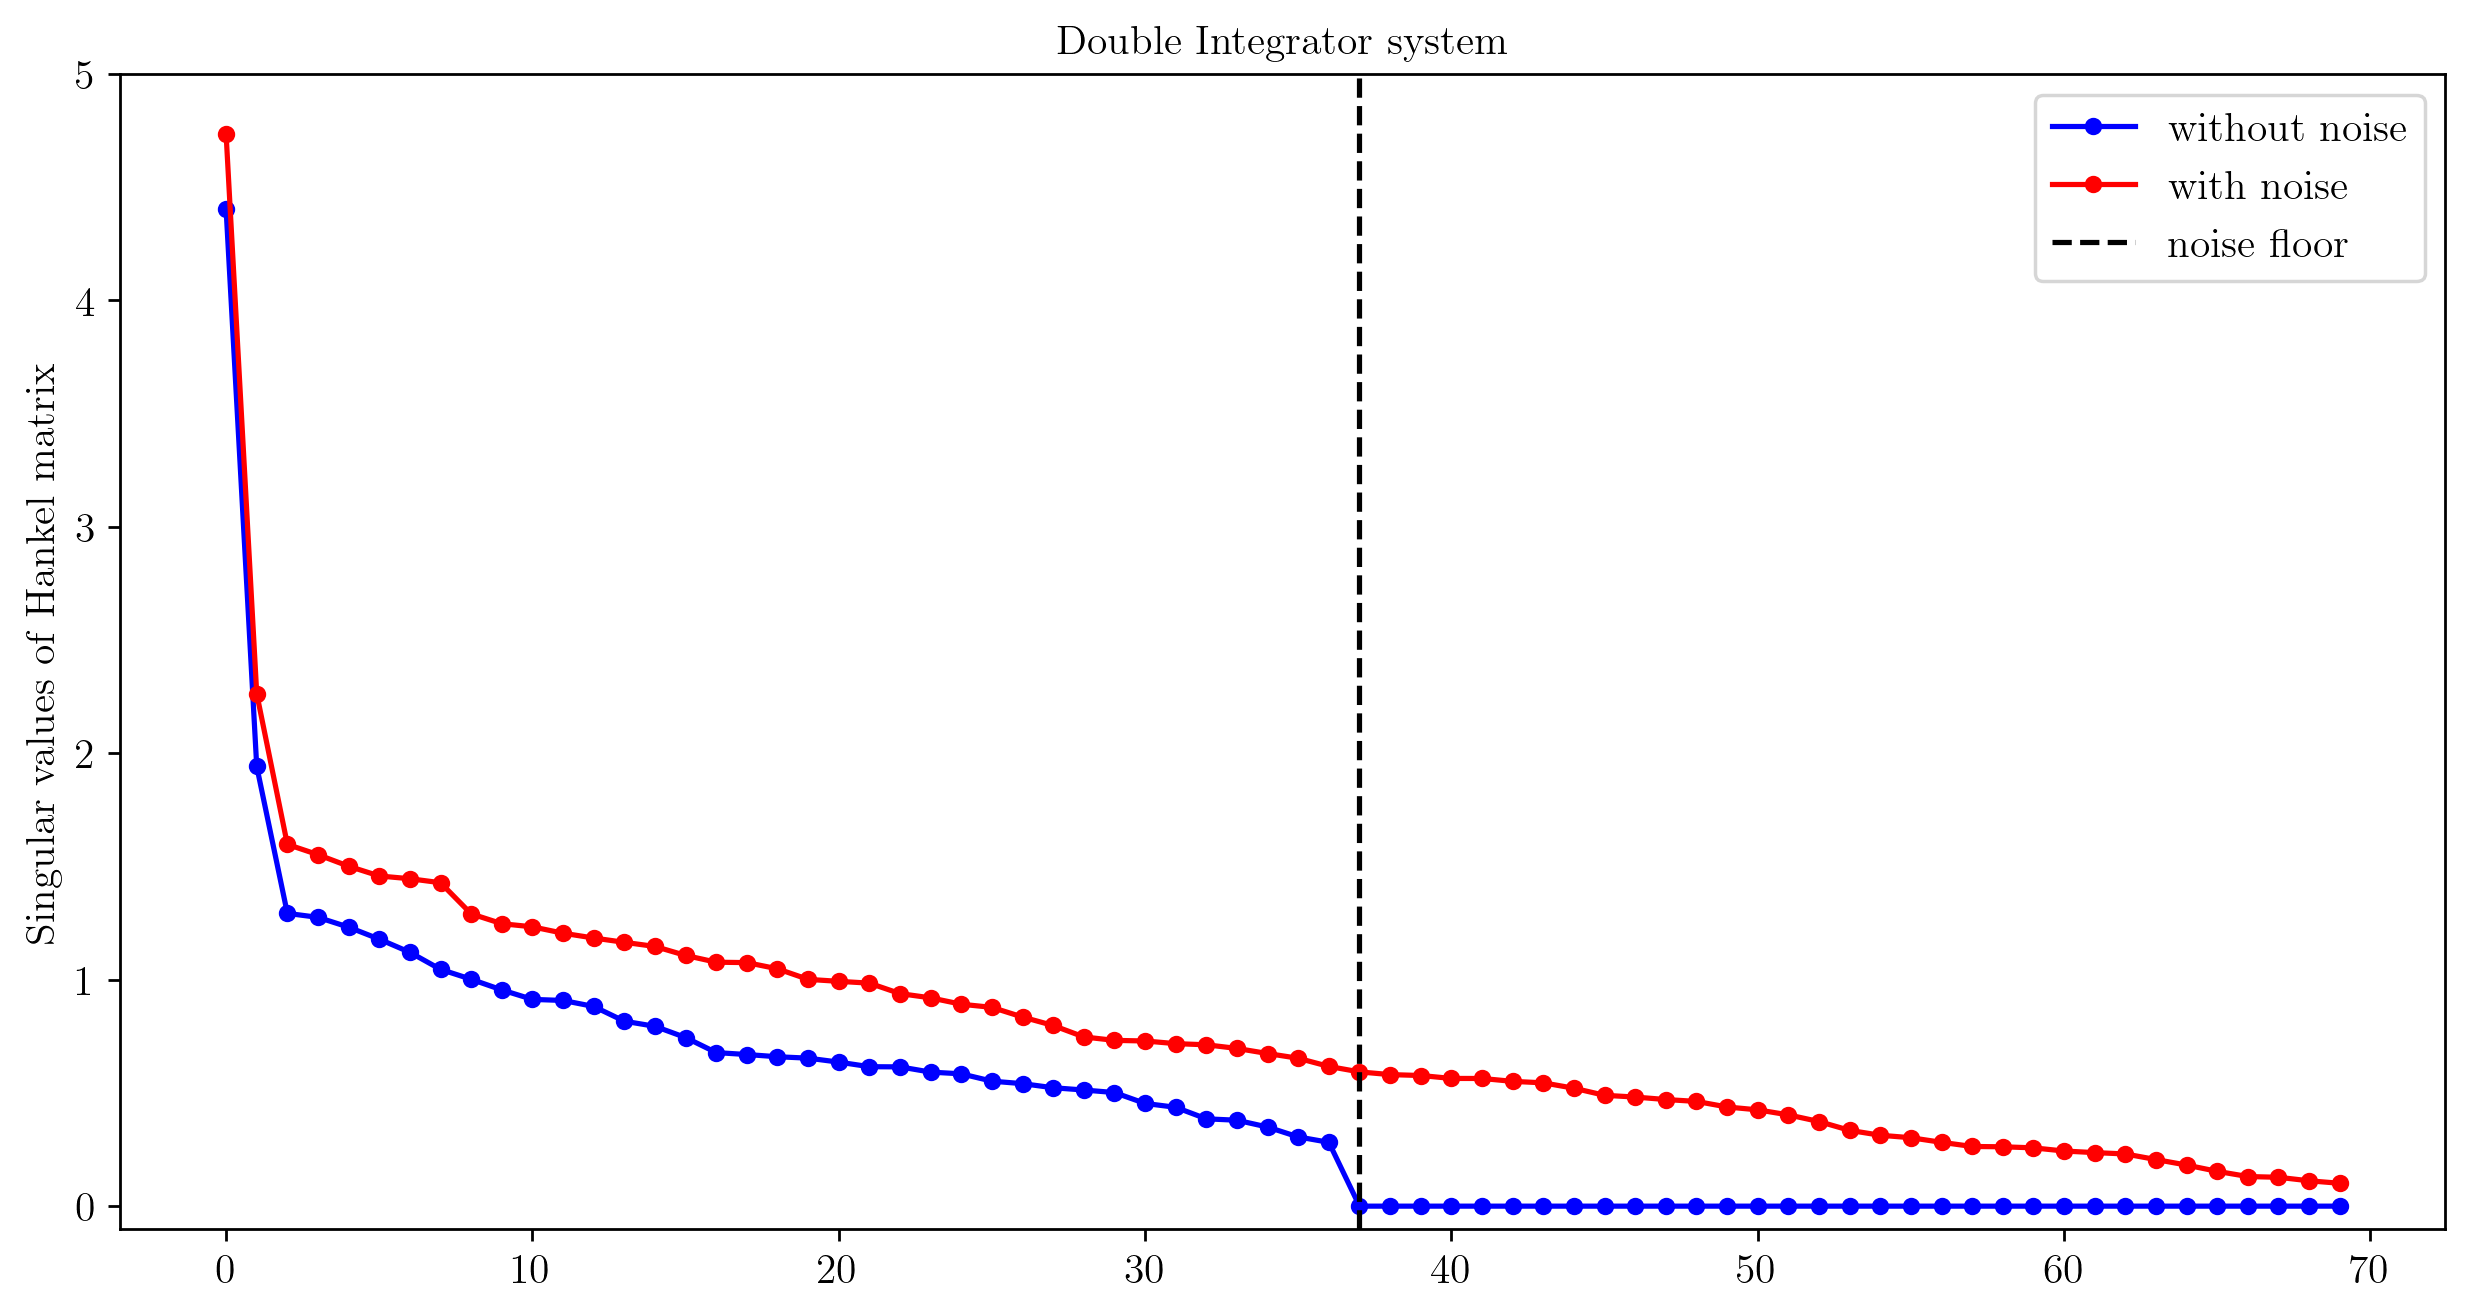
\includegraphics[width=\textwidth]{figures/noise_floor.png}
      \caption{Singular values of Hankel matrices constructed from ideal data (blue) and noisy data (red). The noise floor is shown by the dashed line.}
      \label{fig:svd_noise}
\end{figure}

\subsection{Grassmannians and Behaviors}
Behaviors can be viewed as points on a Grassmannian manifold, which is the space of all $k$-dimensional subspaces of an $n$-dimensional vector space. This perspective allows for the application of geometric methods in system identification and analysis.

Given restricted behavior $\Be|_{[1,L]}$ of dimension $k = m(\Be)L + n(\Be)$, we can associate it with a point on the Grassmannian manifold $\Gr(k, qL)$.

Denote $r_H = \rank \mathcal{H}_L(w)$ for trajectories ${\{w_i\}}_1^{T_d}$. Depending on the noise level, $r_H$ satisfies the following:
\begin{equation}
  k \leq r_H \leq n,
\end{equation}
where $n = qL, k = m(\Be)L + n(\Be)$. Still, only the first $k$ singular vectors of $\mathcal{H}_L(w)$ correspond to the behavior $\Be$. Thus, the behavior can be identified with a point on the Grassmannian manifold $\Gr(k, n)$. To obtain an orthonormal basis for the behavior, we can perform an SVD on $\mathcal{H}_L(w)$ and extract the first $k$ left singular vectors. This basis spans the same subspace as $\Be|_{[1,L]}$, providing a representation of the behavior in the presence of noise. Thus,
\begin{equation}
   \mathcal{H}_L(w) = U \Sigma V^\top,
\end{equation}
where $U \in \R^{n \times r_H}$, $\Sigma \in \R^{r_H \times r_H}$, and $V \in \R^{(T_d-L+1) \times r_H}$. The first $k$ columns of $U$, is equivalently denoted by $\hat{Y}$ such that
\begin{equation}
   \hat{Y} \equiv U_{[1:k]},
\end{equation}
where $\hat{Y} \in \R^{n \times k}$ and $\hat{Y}^\top \hat{Y} = \I_k$. The subspace spanned by the columns of $\hat{Y}$ corresponds to the behavior $\Be|_{[1,L]}$, is also identified by $\hat{S} \in \Gr(k,n)$.

\subsubsection{Summary}
\begin{figure}[h]
   \centering
\begin{tikzpicture}[scale=0.6]
   \node (data) [draw, rectangle, minimum width=3cm, minimum height=1cm] {Collect data $w = \{w_1, \cdots, w_{T_d}\} \in {(\R^{q})^{T_d}}$};
   \node (hankel) [draw, rectangle, minimum width=3cm, minimum height=1cm, below=1.5cm] { $\mathcal{H}_L(w) \in \R^{qL \times (T_d-L+1)}$};
   \node (svd) [draw, rectangle, minimum width=3cm, minimum height=1cm, below=3.5cm] {$\mathcal{H}_L(w) = U \Sigma V^\top$};
   \node (grassmannian) [draw, rectangle, minimum width=3cm, minimum height=1cm, below=5.5cm] {$\Be|_{[1,L]} \equiv \hat{S} \in \Gr(k,n)$};
   \draw[->] (data) -- (hankel) node[midway, right] {Construct Hankel matrix};
   \draw[->] (hankel) -- (svd) node[midway, right] {Perform SVD};
   \draw[->] (svd) -- (grassmannian) node[midway, right] {Extract $\hat{Y} = U_{[1:k]}$};
\end{tikzpicture}
\end{figure}





\chapter{Data-Driven Control}~\label{ch:DDC}
Data-driven control is an emerging paradigm in control theory that focuses on designing controllers directly from data, without relying on explicit parametric models of the system dynamics. This chapter explores the principles and methodologies of predictive control, both in the context of known system models and in scenarios where only data is available. We focus specifically on finite-time linear quadratic tracking problems, and highlight the advantages of the behavioral framework in enabling data-driven control strategies.

\section{Linear Quadratic Tracking}
Finite-time linear quadratic tracking (LQT) is a fundamental optimal control problem~\cite{anderson2007} where the objective is to minimize a quadratic cost function over a finite time horizon while tracking a desired reference trajectory. Consider a discrete-time \Nref*{def:lti} given by 
\begin{equation}
    \begin{cases}
        x(t+1) = A x(t) + B u(t), \\
        y(t) = C x(t) + D u(t),
    \end{cases}
\end{equation}
where $A \in \R^{n \times n}, B \in \R^{n \times m}, C \in \R^{p \times n}, D \in \R^{p \times m}$ are system matrices, $x(t) \in \R^n$ is the state vector, $u(t) \in \R^m$ is the control input, and $y(t) \in \R^p$ is the output vector. Given a desired trajectory $r = (r_0, r_1, \cdots) \in (\R^p)^\N$, input constraint set $\mathcal{U} \subseteq \R^m$, and output constraint set $\mathcal{Y} \subseteq \R^p$, we wish to apply control inputs such that the output tracks the reference trajectory while satisfying the constraints and optimizing a cost function.

In the case where the system is \emph{known}, i.e., the matrices $A, B, C, D$ are given, the finite-horizon LQT problem is approached using \emph{Model Predictive Control}.

\subsection{Model Predictive Control}\label{sec:mpc}
Model Predictive Control (MPC) is an advanced control strategy that utilizes an explicit model of the system to predict future behavior and optimize control actions over a finite horizon~[\cite{camacho2007},~\cite{ferramosca2009}]. Consider the optimization problem:
\begin{equation}\label{eq:mpc}
    \begin{aligned}
        & \underset{u,x,y}{\text{minimize}} && \sum_{k=0}^{N-1} \left( \lVert y_k - r_{t+k} \rVert_Q^2 + \lVert u_k \rVert_R^2 \right) \\
        & \text{subject to} && x_{k+1} = A x_k + B u_k, \\
        & && y_k = C x_k + D u_k, \\
        & && x_0 = \hat{x}(t), \\
        & && u_k \in \mathcal{U}, \forall k \in \{0, \ldots, N-1\} \\
        & && y_k \in \mathcal{Y}, \forall k \in \{0, \ldots, N-1\},
    \end{aligned}
\end{equation}
where $N \in \Z_{> 0}$ is the time horizon, $u = (u_0, u_1, \ldots, u_{N-1}), x = (x_0, x_1, \ldots, x_N)$, $y = (y_0, y_1, \ldots, y_{N-1})$ are the decision variables, and $r_{t+k}$ is the desired reference at time $t+k$, where $t \in \Z_{>0}$ is the time at which the optimization is solved. The matrices $Q \succeq 0$ and $R \succ 0$ are weighting matrices for the output tracking error and control effort, respectively. The initial state $\hat{x}(t)$ is typically obtained from state estimation or measurement at time $t$.

The classical MPC algorithm operates in a \emph{receding horizon} fashion. The algorithm is summarized in Algorithm~\ref{alg:mpc} and illustrated in Figure~\ref{fig:mpc_schematic}.

\begin{algorithm}[H]
\SetKwInOut{Input}{Input}
        \Input{$(A,B,C,D)$, reference trajectory $r$, past input/output data $(u,y)$, constraint sets $\mathcal{U}, \mathcal{Y}$, weighting matrices $Q,R$, time horizon $N$}
    \BlankLine
        Generate state estimate $\hat{x}(t)$ from past data $(u,y)$.\;
        Solve~\eqref{eq:mpc} for $u^* = (u_0^*, u_1^*, \ldots, u_{N-1}^*)$.\;
        Apply inputs $(u(t), \ldots, u(t+s)) = (u^*_0, \ldots, u^*_s)$ for some $s \leq N-1$.\;
  	    Set $t$ to $t+s$ and update past input/output data.\;
        Return to start.
    \caption{Model Predictive Control}
    \label{alg:mpc}
\end{algorithm}

\begin{figure}[h!]
    \centering
    \begin{tikzpicture}[
    scale=1.5,
    >=Stealth,
    timeline/.style={thick, ->},
    horizon/.style={decorate, decoration={brace, amplitude=5pt}},
    trajectory/.style={},
    ref trajectory/.style={trajectory, black, ultra thick, dotted, dash pattern=on 2pt off 10pt},
    actual trajectory/.style={trajectory, red, ultra thick, dotted, dash pattern=on 2pt off 10pt},
    control trajectory/.style={trajectory, blue, thin},
    futcontrol trajectory/.style={trajectory, blue, thin, dashed},
    time label/.style={font=\small}
    ]

    \def\Tini{3}   % Past horizon
    \def\N{5}      % Future horizon
    \def\L{8}      % Total horizon = Tini + N
    \def\usteps{%
    (0,0.50) -- (0.5,0.50)
    -- (0.5,0.5) -- (1.0,0.5)
    -- (1.0,0.35) -- (1.5,0.35)
    -- (1.5,0.75) -- (2.0,0.75)
    -- (2.0,0.45) -- (2.5,0.45)
    -- (2.5,0.65) -- (3.0,0.65)
    }
    \def\futsteps{
    (3.0, 0.65) -- (3.0,0.50) -- (3.5,0.50)
    -- (3.5,0.50) -- (4.0,0.50)
    -- (4.0,0.50) -- (4.5,0.50)
    -- (4.5,1.2) -- (5.0,1.2)
    -- (5.0,0.58) -- (5.5,0.58)
    -- (5.5,0.75) -- (6.0,0.75)
    -- (6.0,0.35) -- (6.5,0.35)
    -- (6.5,0.47) -- (7.0,0.47)
    -- (7.0,0.47) -- (7.5,0.47)
    -- (7.5,0.47) -- (8.0,0.47)
    }

    \draw[gray!80, timeline] (-0.5, 0) -- (\L+0.5, 0);


    \draw[gray!80, thin] (3, 0.2) -- (3, -0.2) node[below, time label] {$k$};
    \draw[gray!80, thin] (8, 0.2) -- (8, -0.2) node[below, time label] {$N$};


    \draw[->, gray!80, thick] (\Tini, -0.1) -- (\Tini, 4);

    \draw[ref trajectory] (0, 2) to[out=0, in=170] (\L, 2.7) node[above left, yshift=2mm] {reference $\mathbf{r}$};
    \draw[trajectory] (0, 2) to[out=0, in=170] (\L, 2.7);


    \draw[actual trajectory] (0, 1) to[out=10, in=170] 
        (\L, 2.5) node[below left] {output $\mathbf{y}$};
    \draw[trajectory, red] (0,1) to [out=8, in=19] (\Tini, 1.84);
    \draw[thin, densely dashed, red] (0,1) to[out=10,in=170] (\L, 2.5);

    \draw[control trajectory] \usteps;
    \draw[futcontrol trajectory] \futsteps node[above left, yshift=5mm] {control action $\mathbf{u}$};


    \node at (\Tini/1.5, 3.9) {\textcolor{gray}{past}};
    \draw[<-, gray!80] (\Tini/1.5-0.7, 3.6) to (\Tini/1.5+0.7, 3.6);
    \node at (\Tini + \N/5, 3.9) {\textcolor{gray}{future}};
    \draw[->, gray!80] (\Tini+\N/5-0.7, 3.6) to (\Tini+\N/5+0.7, 3.6);

    \draw[<->, gray!80] (\Tini, -0.8) to (8,-0.8) node[below left] {\textcolor{gray}{prediction horizon}};

    \end{tikzpicture}
    \caption{Classical MPC in a receding horizon fashion. At each time step, an optimization problem is solved over a future horizon using the current state estimate and past data. The first $s$ control inputs are applied, and the horizon recedes forward in time.}~\label{fig:mpc_schematic}
\end{figure}

\newpage
\subsection{Data-Driven Predictive Control}

When the system model is \emph{unknown}, i.e., the matrices $A, B, C, D$ are not available, traditional model-based control strategies like MPC cannot be directly applied. Instead, we turn to data-driven predictive control methods [e.g. DeePC~\cite{jeremy2019}] that leverage historical input-output data to design controllers without explicit knowledge of the system dynamics. The behavioral framework introduced in Chapter~\ref{ch:Behaviors} provides a powerful toolset for such data-driven approaches, since it bypasses the need for parametric models and directly utilizes data to characterize system behavior.

On a finite-horizon, the problem can be formulated as follows. Given,
\begin{itemize}
    \item an LTI system $\Sigma = (\T, \W, \Be)$, with $\W = \R^q$, and $\T = [1,N]$,
    \item an initial trajectory $w_{\textrm{ini}} \in \Be |_{\T_{\textrm{past}}}$ with $\T_{\textrm{past}} = [1, T_{\textrm{ini}}]$,
    \item a reference trajectory $w_{\textrm{ref}} \in {(\R^q)}^{\T_{\textrm{fut}}}$, with $\T_{\textrm{fut}} = [T_{\textrm{ini}}+1, N]$,
    \item a symmetric positive semi-definite weighting matrix $\Phi \in \R^{q \times q}$,
\end{itemize}
the linear quadratic tracking problem is to find a trajectory $w_{\textrm{fut}} \in \Be |_{\T_{\textrm{fut}}}$ that solves the optimization problem
\begin{equation}\label{eq:lqt_behavioral}
    \begin{aligned}
        \underset{w_{\textrm{fut}} \in {(\R^q)}^{\T_{\textrm{fut}}}}{\text{minimize}} && \sum_{k=T_{\textrm{ini}}+1}^{N} \lVert w_{\textrm{fut}}(k) - w_{\textrm{ref}}(k) \rVert_{I \otimes \Phi}^2 \\
       && \text{subject to} \quad w = \begin{bmatrix} w_{\textrm{ini}} \\ w_{\textrm{fut}} \end{bmatrix} \in \Be.
    \end{aligned}
\end{equation}

\begin{Note}
    The reference trajectory $w_{\textrm{ref}}$ need not be in the behavior $\Be$. For instance, step inputs with sudden changes can be used as reference trajectories, even if they are not achievable by the system.
\end{Note}

If a parametric model of the system behavior is available---for example a state-space representation---then the optimization problem~\eqref{eq:lqt_behavioral} is equivalent~\cite{jeremy2019} to the classical MPC problem~\eqref{eq:mpc} described in Section~\ref{sec:mpc}. However, in the absence of such a model, we can utilize the behavioral framework to reformulate the problem in a data-driven manner.

\section{Robust Least-Squares for Data-Driven Control}
Predictive control methods like DeePC~\cite{jeremy2019} rely on the availability of persistently exciting input-output data to construct Hankel matrices that capture the system's behavior. However, in practical scenarios, the collected data may be corrupted by noise, outliers, or other uncertainties, which can adversely affect the performance of data-driven controllers. To address these challenges, robust least-squares techniques can be employed to enhance the resilience of data-driven predictive control methods against data imperfections.

\subsection{Geometric Approach to Robust Least-Squares}
We consider a geometric approach to robust least-squares problem in the context of linear quadratic tracking. Building up from~\eqref{eq:lqt_behavioral}, we formulate:
\begin{equation}\label{eq:robust_lqt}
    \begin{split}
    \min_{w \in \R^n} & \max_{\Sy \in \B_{\rho}(\hat{\Sy})} \lVert w - w_{\textrm{ref}} \rVert^2 \\
    \text{subject to} & \quad \begin{cases} w \in \Sy,\\
          w|_{\T_{\textrm{past}}} = w_{\textrm{ini}} \end{cases}
    \end{split}
\end{equation}
Here, 
\begin{itemize}
    \item $\B_{\rho}(\hat{\Sy}) \subseteq \Gr(k,n)$ is a ball of radius $\rho$ centered at $\hat{\Sy} \equiv \Be|_{[1,L]}$ which is obtained via behavioral system identification.
    \item $n = qL, k = m(\Be)L+n(\Be)$ where $m(\Be), n(\Be)$ are the output and state dimensions of the behavior $\Be$ respectively.
    \item $w_{\textrm{ref}} = \textrm{col}(w_{\textrm{ini}}, w_{\textrm{ref,f}}) \in {(\R^q)}^\T$ is the reference trajectory over the horizon $N$.
    \item $w_{\textrm{ini}} \in {(\R^q)}^{\T_{\textrm{past}}}$ is the initial trajectory over the horizon $N$.
\end{itemize}

\subsection{Constraints}
The constraints in~\eqref{eq:robust_lqt} are briefly discussed here.

\begin{table}[h]
    \centering
    \begin{tabular}{p{0.46\linewidth}|p{0.46\linewidth}}
        % \hline
        % anchor labels so references like \eqref{const1}/\eqref{const2} work
        % \refstepcounter{equation}\label{const1} (\theequation) & \refstepcounter{equation}\label{const2} (\theequation) \\
        To enforce the constraint $w \in \Sy$, we utilize the orthogonal projection onto the subspace $\Sy$. Specifically, we take the transformation
        \begin{equation}
            w = P_{\Sy} x = YY^\top x,
        \end{equation}
        where $P_{\Sy}$ is the orthogonal projection matrix onto the subspace $\Sy$, and $Y \in \R^{n \times k}$ is an orthonormal basis for $\Sy$. The variable $x \in \R^n$ is a new decision variable that allows us to express $w$ in terms of the subspace $\Sy$. & The past constraint $w|_{\T_{\textrm{past}}} = w_{\textrm{ini}}$ is a linear equality constraint that can be expressed in matrix form as
        \begin{equation}
            M w = w_{\textrm{ini}},
        \end{equation}
        where $M = [\I_{q T_{\textrm{ini}}} \quad 0] \in \R^{q T_{\textrm{ini}} \times n}$ is a selection matrix that extracts the components of $w$ corresponding to the past horizon $\T_{\textrm{past}}$.
        Substituting the expression for $w$ into this constraint gives
        \begin{equation}
            M YY^\top x = w_{\textrm{ini}}.
        \end{equation} 
        % \hline
    \end{tabular}
    \caption{Reformulation of constraints in~\eqref{eq:robust_lqt}.}~\label{tab:constraints_reformulation}
\end{table}

\subsection{Reformulated Problem}
Substituting the expressions for $w$ and the constraints into the robust least-squares problem~\eqref{eq:robust_lqt}, we obtain the reformulated optimization problem:
\begin{equation}\label{eq:reformulated_robust_lqt}
    \begin{split}
    \min_{x \in \R^n} & \max_{\Sy \in \B_{\rho}(\hat{\Sy})} \lVert YY^\top x - b \rVert^2 \\
    \text{subject to} & \quad M YY^\top x = z,
    \end{split}
\end{equation}
where $b = w_{\textrm{ref}}$ and $z = w_{\textrm{ini}}$ for notational convenience. This problem is exactly in the form of the constrained robust least-squares problem discussed in Chapter~\ref{ch:Preliminaries}, Subsection~\ref{subsec:cons-robust-ls}, and can be solved using the geometric approach outlined therein.

\begin{Note}
    The cost function in~\eqref{eq:reformulated_robust_lqt} can be modified to include weighting matrices or regularization terms as needed (see Subsection~\ref{subsec:reg}). For instance, if we wish to penalize deviations in certain components of the trajectory more heavily, we can introduce a weighting matrix $\Phi$ into the cost function.
\end{Note}

Thus, the algorithm for data-driven predictive control using (regularized) robust least-squares can be summarized as follows:

\begin{algorithm}[H]
\SetKwInOut{Input}{Input}\SetKwInOut{Output}{Output}
        \KwData{Subspace estimate $\hat{\Sy} \in \Gr(k,n)$, System simulator $(A,B,C,D)$}
        \Input{Initial trajectory $z = w_{\textrm{ini}} \in {(\R^q)}^{\T_{\textrm{ini}}}$, Reference trajectory $r \in {(\R^p)}^{\T}$}
        \Output{Optimal trajectories $w^* \in {(\R^q)}^{\T}$}
    \BlankLine\While{$t \in [1,T]$} {
        Update $z = w_{\textrm{ini}} = [u_{\textrm{past}}^\top, y_{\textrm{past}}^\top]^\top$ from past data.\;
        Update $w_{\textrm{ref,f}} = [0^\top, r^\top]^\top$ from reference data.\;
        Define $b = [z^\top, w_{\textrm{ref,f}}^\top]^\top$.\;
        Solve Algorithm~\ref{alg:cons-robust-ls} with inputs $(\hat{\Sy}, b, z)$ to obtain $(x^*,Y^*)$.\;
        Obtain optimal trajectory $w^* = Y^* {Y^*}^\top x^*$.\;
        Apply control inputs $u^*(t), \ldots, u^*(t+s)$ for some $s \leq N-1$.\;
        Set $t$ to $t+s$ and update past input/output data.\;
    }
    \caption{Data-Driven Predictive Control via Robust Least-Squares}
\end{algorithm}

\section{Results}
The proposed data-driven predictive control algorithm using robust least-squares has been evaluated on various LTI systems. The results demonstrate improved tracking performance and robustness against data imperfections compared to traditional least-squares approaches. 

\subsection{Double Integrator System}
Consider a simple double-integrator system $\ddot{x}(t) = \dfrac{F(t)}{m}$, given in discrete time as
\begin{equation}
\begin{split}
    \begin{bmatrix}
        x_{k+1} \\ v_{k+1}
    \end{bmatrix} &= \begin{bmatrix}
        1 & h \\ 0 &  1
    \end{bmatrix} \begin{bmatrix}
        x_k \\ v_k
    \end{bmatrix} + \begin{bmatrix}
        \frac{h^2}{2m} \\ \frac{h}{m}
    \end{bmatrix}u_k  \\
    y_k &= \begin{bmatrix}
        1 & 0
    \end{bmatrix} \begin{bmatrix}
        x_k \\ v_k
    \end{bmatrix} + \eta_k
\end{split}
\end{equation}
where $x_k = x(t_k), v_k = \dot{x}(t_k)$ are the states, $h = t_{k+1} - t_k$ is the simulation time-step, and $\eta_k \sim \mathcal{N}(0, \sigma^2)$ is measurement noise. The system parameters are set to $m = 1$ kg, $h = 0.5$ s. The control objective is to track a reference trajectory $r = 1$ m over a horizon of $N$ time steps, with a random initial condition $[x_0, v_0]$.

\subsubsection{Offline System Identification}
To identify the behavior $\Be$ of the double-integrator system, we collect input-output data by simulating the system with random control inputs $u_k$ drawn from a uniform distribution over $[-1, 1]$ N. The output measurements $y_k$ are corrupted with Gaussian noise. A total of $T = 115$ time steps of data is collected, and a persistently exciting input sequence of order $L = T_{\textrm{ini}}+N = 35$ is ensured. Using this data, we construct the Hankel matrix and extract the subspace estimate $\hat{\Sy}$ using the methods outlined in Chapter~\ref{ch:Behaviors}. Thus, we summarize the following parameters from system identification of the double-integrator system in Table~\ref{tab:sysid_params_double_integrator}.
\begin{table}[h]
    \centering
    \begin{tabular}{l|c}
        \textbf{Parameter} & \textbf{Value} \\
        \hline 
        \hline
        Number of inputs $m(\Be)$ & 1 \\
        Number of outputs $p(\Be)$ & 1 \\
        Number of states $n(\Be)$ & 2 \\
        Dimension of behavior $k$ & 37 \\
        Data length $T_d$ & 115 \\
        Future horizon $N$ & 25 \\
        Past horizon $T_{\textrm{ini}}$ & 10 \\
        Total horizon $L$ & 35 \\
        Subspace dimension $\dim(\hat{Y})$ & 70 $\times$ 37 \\
        \hline
    \end{tabular}
    \caption{System identification parameters for double-integrator system.}~\label{tab:sysid_params_double_integrator}
\end{table}

\subsubsection{Online Predictive Control}
With the identified subspace $\hat{\Sy}$, we implement the data-driven predictive control algorithm using robust least-squares. The control inputs are computed over a receding horizon of $T = 50$ time steps, with the first $s = 1$ control input applied at each iteration. The reference trajectory is set to $r_k = 1$ m for all $k$. The robust least-squares problem is solved using the geometric approach outlined in Chapter~\ref{ch:Preliminaries}, with a ball radius $\rho$ chosen based on the noise level in the data.

Figures~\ref{fig:ddpc_noiseless} and~\ref{fig:conv_noiseless} illustrate the system simulations and optimization convergence for the case of no measurement noise ($\sigma = 0$). The results demonstrate effective tracking of the reference trajectory and convergence of the optimization process. The parameters/results for the simulations are summarized in Table~\ref{tab:ddpc_params_double_integrator}.
\begin{table}[h]
    \centering
    \begin{tabular}{l|c}
        \textbf{Parameter} & \textbf{Value} \\
        \hline 
        \hline
        $\rho$ & 0.1$^\circ$ \\
        $\gamma$ & 5.0 \\
        Total Run-Time & 4.27 s \\
        Tracking Time & 15 s \\
        \hline
    \end{tabular}
    \caption{Simulation parameters/results for $\sigma=0$ (no noise)}
    \label{tab:ddpc_params_double_integrator}
\end{table}
\begin{figure}[h]
    \centering
    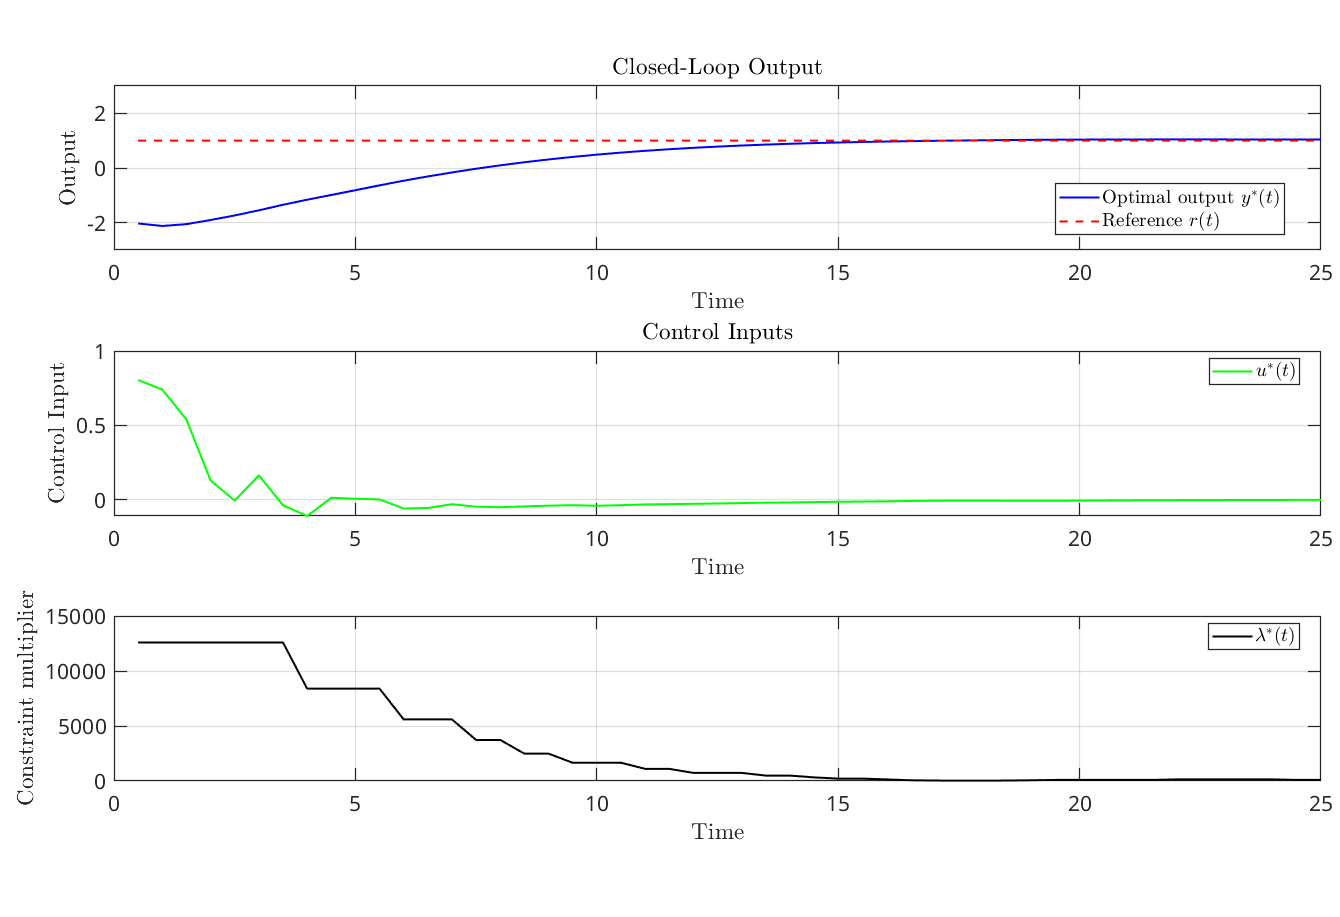
\includegraphics[trim={0cm 1cm 0cm 0cm},clip,width=\textwidth]{figures/closed_loop_noiseless_gamma_5_rho_0p1.png}
    \caption{System simulations for $\sigma = 0$ (no noise).}\label{fig:ddpc_noiseless}
\end{figure}

\textbf{Observations}:
\begin{itemize}
    \item Initially, $\lambda^*$ is large, indicating a significant deviation from the reference trajectory. As the optimization progresses, $Y^*$ aligns better with the true behavior $\hat{Y}$, leading to a decrease in $\lambda^*$.
    \item The optimization algorithm converges within $\sim 30$ iterations per time step on average, demonstrating computational efficiency suitable for real-time applications.
    \item The choice of ball radius $\rho$ significantly impacts the robustness of the control strategy.
\end{itemize}
\begin{figure}[h!]
    \centering
    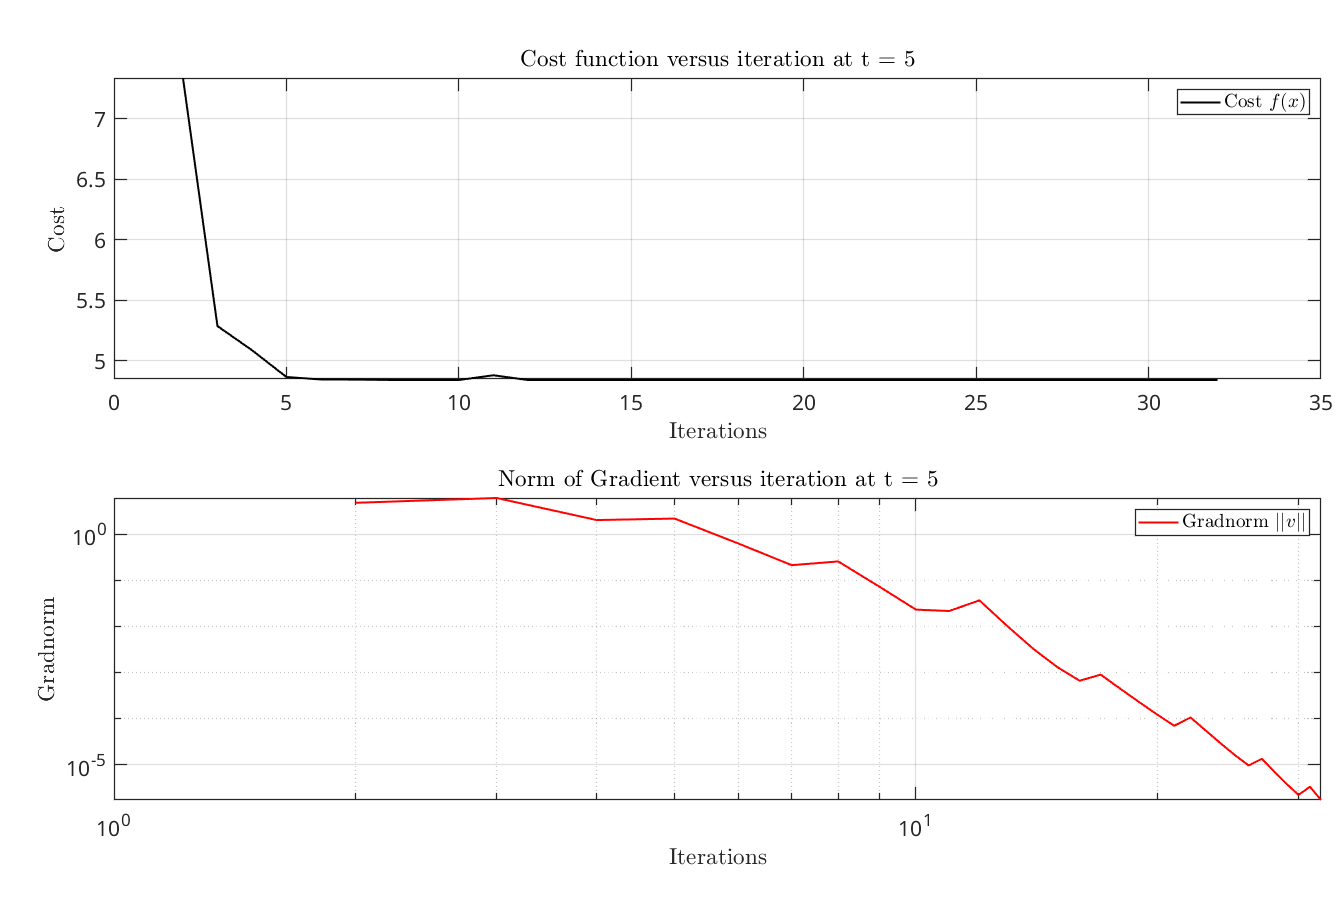
\includegraphics[width=0.9\textwidth]{figures/cost_gradnorm_noiseless_gamma_5_rho_0p1.png}
    \caption{Optimization algorithm convergence at $t=5s$ for $\sigma = 0$ (no noise).}
    \label{fig:conv_noiseless}
\end{figure}

Next, we consider the case with measurement noise ($\sigma = 0.1$). Figures~\ref{fig:ddpc_noisy1} and~\ref{fig:conv_noisy1} illustrate the system simulations and optimization convergence for this scenario. The results show that the robust least-squares approach effectively mitigates the impact of noise, achieving satisfactory tracking performance. The parameters/results for the noisy simulations are summarized in Table~\ref{tab:ddpc_params_double_integrator_noisy1}.
\begin{figure}[h!]
    \centering
    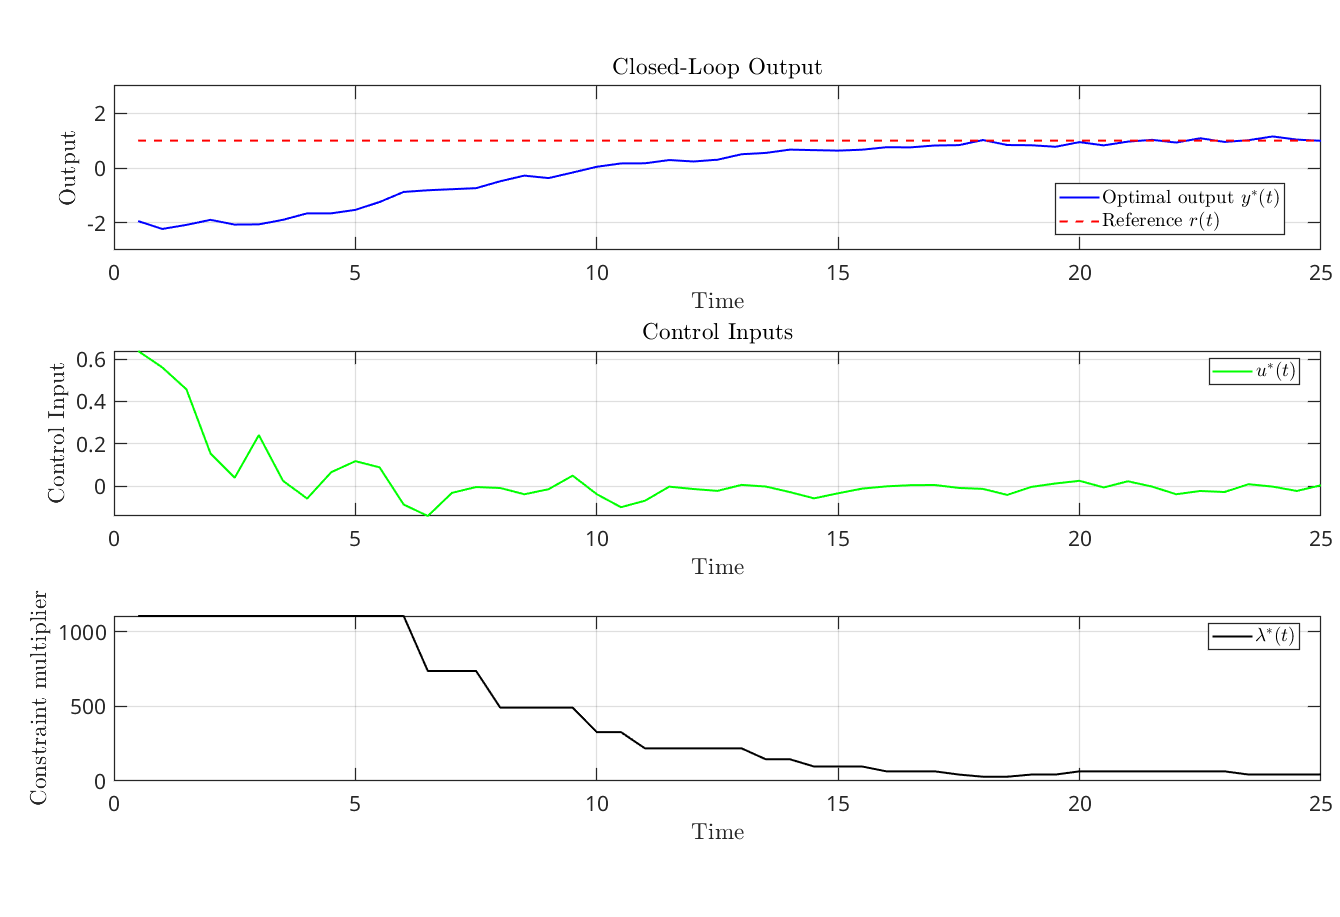
\includegraphics[trim={0cm 1cm 0cm 0cm},clip,width=0.9\textwidth]{figures/closed_loop_snr_0p1_gamma_4_rho_1.png}
    \caption{System simulations for $\sigma = 0.1$ (with noise).}
    \label{fig:ddpc_noisy1}
\end{figure}

\begin{figure}[h]
    \centering
    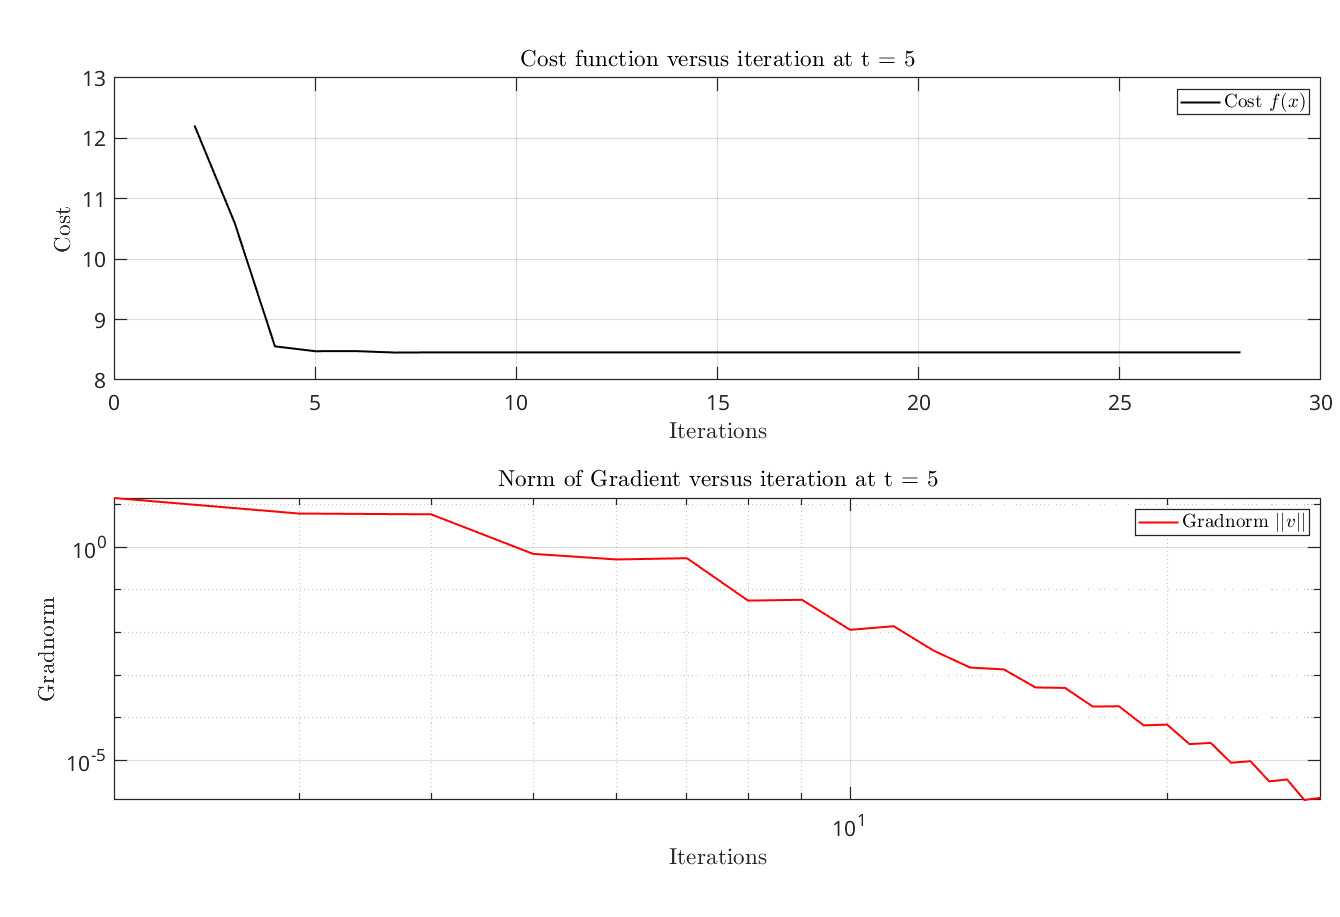
\includegraphics[width=\textwidth]{figures/cost_gradnorm_snr_0p1_gamma_4_rho_1.png}
    \caption{Optimization algorithm convergence at $t=5s$ for $\sigma = 0.1$ (with noise).}
    \label{fig:conv_noisy1}
\end{figure}

\newpage
\begin{table}[h]
    \centering
    \begin{tabular}{l|c}
        \textbf{Parameter} & \textbf{Value} \\
        \hline 
        \hline
        $\rho$ & 1$^\circ$ \\
        $\gamma$ & 4.0 \\
        Total Run-Time & 5.46 s \\
        Tracking Time & 18 s \\
        \hline
    \end{tabular}
    \caption{Simulation parameters/results for $\sigma=0.1$ (with noise)}
    \label{tab:ddpc_params_double_integrator_noisy1}
\end{table}

Now, we further increase the measurement noise to $\sigma = 0.5$. Figures~\ref{fig:ddpc_noisy2} and~\ref{fig:conv_noisy2} illustrate the system simulations and optimization convergence for this higher noise scenario. The robust least-squares approach continues to provide effective tracking performance despite the increased noise level. The parameters/results for the high-noise simulations are summarized in Table~\ref{tab:ddpc_params_double_integrator_noisy2}.

\begin{figure}[h!]
    \centering
    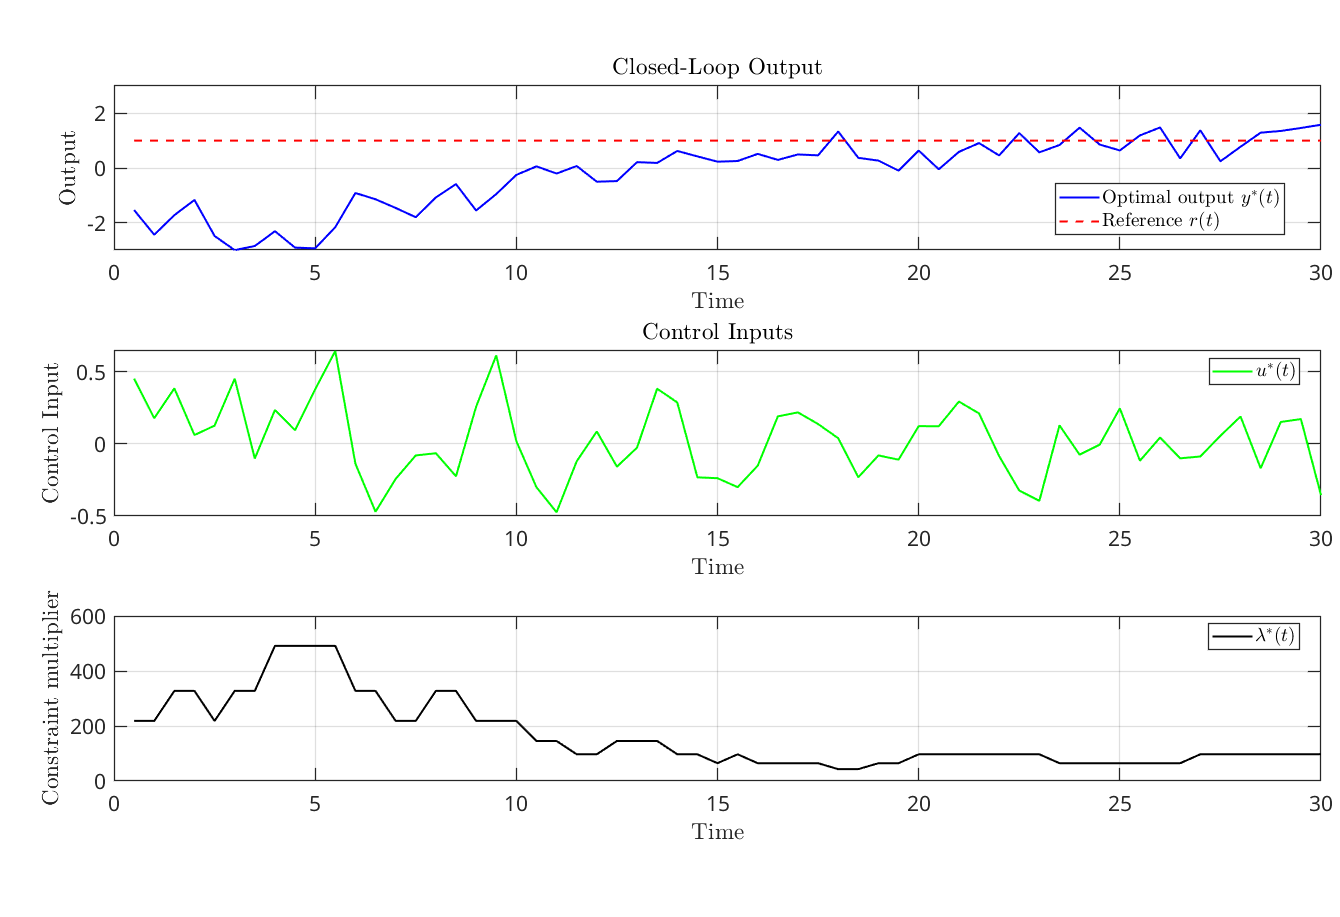
\includegraphics[width=\textwidth]{figures/closed_loop_snr_0p5_gamma_5_rho_3p5.png}
    \caption{System simulations for $\sigma = 0.5$ (with noise).}
    \label{fig:ddpc_noisy2}
\end{figure}
\begin{figure}[h!]
    \centering
    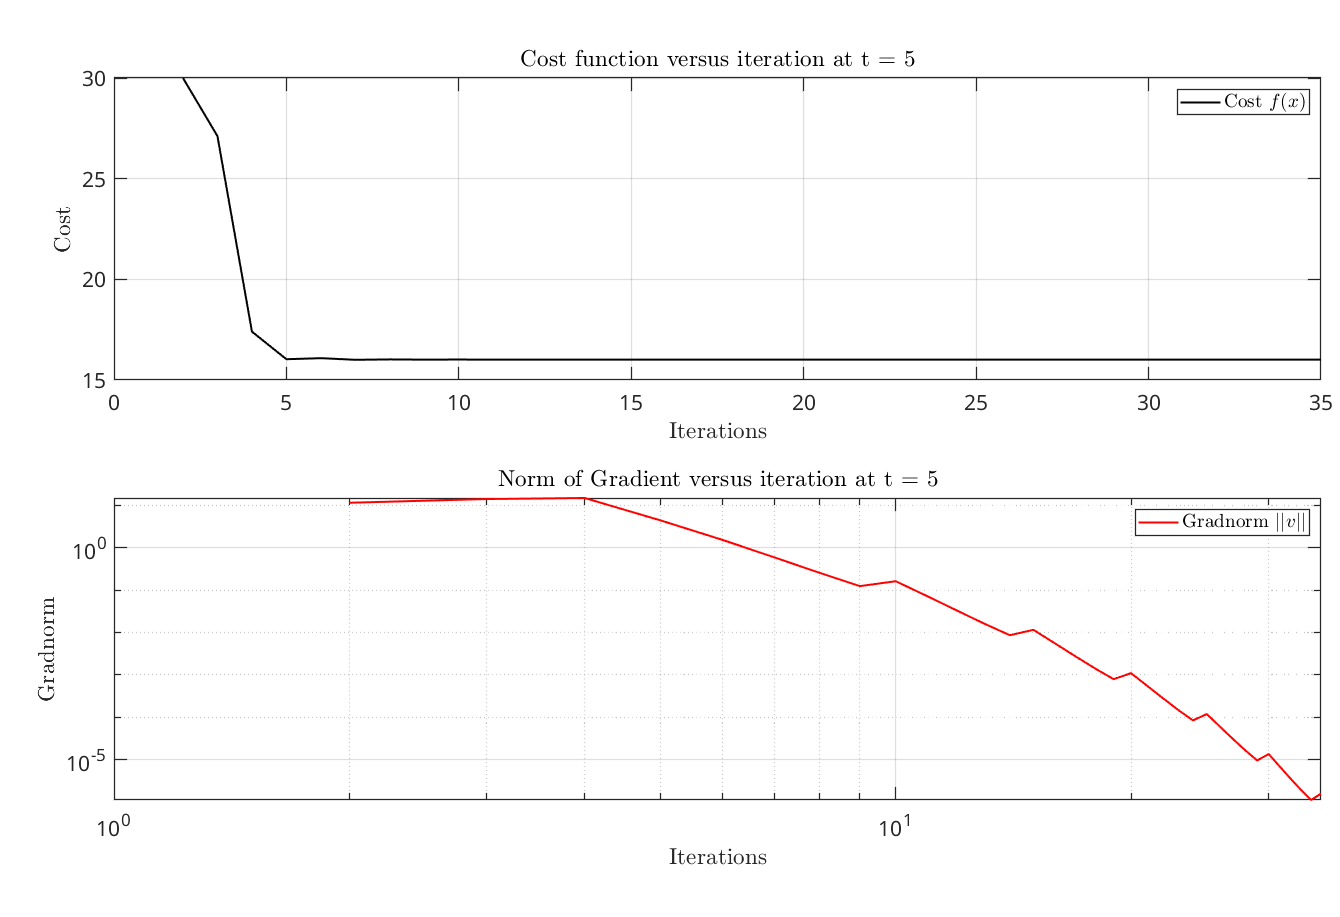
\includegraphics[width=\textwidth]{figures/cost_gradnorm_snr_0p5_gamma_5_rho_3p5.png}
    \caption{Optimization algorithm convergence at $t=5s$ for $\sigma = 0.5$ (with noise).}
    \label{fig:conv_noisy2}
\end{figure} 

\begin{table}[h]
    \centering
    \begin{tabular}{l|c}
        \textbf{Parameter} & \textbf{Value} \\
        \hline 
        \hline
        $\rho$ & 3.5$^\circ$ \\
        $\gamma$ & 5.0 \\
        Total Run-Time & 10.66 s \\
        Tracking Time & 20 s \\
        \hline
    \end{tabular}
    \caption{Simulation parameters/results for $\sigma=0.5$ (with high noise)}
    \label{tab:ddpc_params_double_integrator_noisy2}
\end{table}

\clearpage
\textbf{Observations}:

\begin{itemize}
    \item As the noise level increases, the choice of $\rho$ becomes more critical to maintain robust tracking performance. Remark~\ref{rem:rho} provides insights on how $\rho$ has been estimated in the simulations.
    \item The optimization algorithm remains effective, converging within a reasonable number of iterations even under high noise conditions.
    \item Tuning $\gamma$ helps balance controller performance and algorithm convergence speed. It is yet to be understood how to perform a dynamic update of $\gamma$ during the optimization process for improved results.
\end{itemize}

\begin{remark}\label{rem:rho}
    The ball radius $\rho$ is the quantification of uncertainty in the behavioral estimate $\hat{\Sy}$ (or $\hat{Y}$). As one may expect, increase in measurement noise $\sigma$ should lead to an increase in $\rho$. Although an exact relationship between $\sigma$ and $\rho$ is not yet established, one may estimate $\rho$ as follows.

    Assuming only measurement noise $\eta_k$, denote $\hat{w}_k \in \R^q$ as the noise-free trajectory at time $k$, and $w_k = \hat{w}_k + e_k$ as the actual trajectory, such that
    \[
        e_k = \begin{bmatrix}
            0 \\ \eta_k
        \end{bmatrix} \in \R^q.
    \]
    Let $\hat{Y}$ be the behavioral estimate obtained from system identification (also corrupted by noise). Thus, for online control, the worst-case subspace should contain the worst-case trajectory $w_k$. Note that here, we can assume $\hat{w}_k \in \hat{\Sy}$.  Hence,
    \[
        \rho \approx d_{\infty}(\hat{Y}, Y^*) = \sin(\theta),
    \]
    where $\theta$ is the maximum principle angle between the subspaces $\hat{\Sy}$ and $\Sy_k$ that contains the worst-case trajectory $w_k$. Using basic trigonometry, we thus have
    \[
        \theta = \max_{k} \left\{ \tan^{-1} \left(\dfrac{\lVert P_{\hat{\Sy}}^{\perp} e_k \rVert}{\lVert \hat{w}_k + P_{\hat{\Sy}} e_k \rVert} \right) \right\}.
    \]
\end{remark}

\begin{figure}[h!]
    \centering
    \begin{tikzpicture}[x={(1cm,0cm)}, y={(0.5cm,0.5cm)}, z={(0cm,1cm)}, scale=1.5, >=Stealth]
\fill[blue!20, opacity=0.8] (0,-0.5,0) -- (4,-0.5,0) -- (4,1.5,0) -- (0,1.5,0) -- cycle;
\draw[blue!50, thick] (0,-0.5,0) -- (4,-0.5,0) -- (4,1.5,0) -- (0,1.5,0) -- cycle;
\node at (3.5,0.3,0) {$\hat{\mathcal{S}}$};

\draw[->, thick, blue] (0,0,0) -- (2.8,0.7,0) node[midway, below right ] {$\hat{w}_k$};

\fill[red!30, opacity=0.8, rotate=20] (0,-0.5,0) -- (4.5,-0.5,0) -- (4.5,1.5,0) -- (0,1.5,0) -- cycle;
\draw[red!50, thick, rotate=20] (0,-0.5,0) -- (4.5,-0.5,0) -- (4.5,1.5,0) -- (0,1.5,0) -- cycle;

\draw[->, thick, red] (0,0,0) -- (3.5,1,1) node[midway, above left] {$w_k$};
\node at (3.7,1,1.5) {$\mathcal{S}_k$};

\draw[->,thick,purple] (2.8,0.7,0) -- (3.5,1,1) node[midway, right] {$e_k$};
\draw[dashed, purple] (3.5,1,0) -- (3.5,1,1) node[midway, right] {$P_{\hat{\mathcal{S}}}^{\perp} e_k$};
\draw[thick, purple] (3.4,1,0.1) -- (3.5,1,0.15);
\draw[thick, purple] (3.4, 1,0.11) -- (3.4,1.01,-0.05);

\node at (0.9,0,0.23) {$\theta$};
\path[clip] (2,0.5,0) -- (0,0,0) -- (2,1,0.4) -- cycle;
\node[circle,draw=black,minimum size=60pt,thick] at (0,0,0) (circ) {};

\end{tikzpicture}
\caption{Estimation of ball radius $\rho$ based on trajectory deviation $e_k$.}
\end{figure}

\backmatter{}
%% NOTE: uncomment following line if you use parts in your document
% \addtocontents{toc}{\vspace{2ex}}  % Add extra space after the last part in TOC

\chapternotnumbered{Summary and Future Work}

\label{ch:Summary}
\vspace{2ex}
This thesis has explored the application of robust least-squares optimization in the context of data-driven predictive control, leveraging the behavioral approach to systems theory. By representing dynamical systems based on observed input-output data, we have developed a geometric framework that effectively handles uncertainties in system dynamics.

The key contributions of this work include:
\begin{enumerate}
    \item Development of a robust least-squares optimization framework that accounts for subspace uncertainty, enabling more reliable control strategies in the presence of data perturbations.
    \item Integration of the behavioral approach to system theory, allowing for a flexible representation of dynamical systems without explicit parametric models.
    \item Formulation of data-driven predictive control problems as constrained least-squares problems, facilitating the design of control strategies directly from observed data.
    \item Demonstration of the effectiveness of the proposed framework through numerical simulations.
\end{enumerate}

Future research directions include:
\begin{itemize}
    \item Extension of the robust least-squares framework to accommodate linear time-varying (LTV) systems and nonlinear systems.
    \item System-theoretic interpretation of the worst-case subspace $Y^\star$ in the context of robust or $H_\infty$ control.
    \item Enhancing the computational efficiency of the proposed algorithms using advanced optimization techniques like adaptive time-stepping, etc.
    \item Experimental validation of the proposed framework on real-world systems to assess its practical applicability and performance.
\end{itemize}

% \appendix
% \chapter{Example of Appendix Chapter} \label{appendix:example}

% \begin{example}[Figure Caption Tweaking]
%     Now we will show off some figures with tweaked position/extent of the captions.
%     \Cref{fig:parallel-plate-capacitor} has a side-caption, while \Cref{fig:tighter_caption} has a caption that spans just the width of the figure.
%     This utilizes the \package{floatrow} package and is inspired by the ITT \LaTeX{} template \autocite{ITTtemplate}.
% \end{example}

% \begin{figure}[!ht]
%     \exportInkscapeSVG{parallel-plate-capacitor}% export already here, such that we can use it in the caption
%     \fcapside[\FBwidth]{%
%         \caption[Example of a figure with a side-caption.]{
%             Example of a figure with a side-caption.

%             It displays the two-dimensional electric field near one end of a parallel plate capacitor.
%             \vspace{1ex}

%             \textbf{\textsf{Legend:}}\\[0.4ex]
%             \begin{tblr}{stretch=0.8, column{1} = {rightsep=2pt, cmd=\raisebox{-0.31ex}}}
%                 \adjincludegraphics[width=0.6\textwidth, Clip={0.87\width} {0.483\height} {0.0\height} {0.483\height}]{parallel-plate-capacitor} & equipotentials  \\
%                 \adjincludegraphics[width=0.6\textwidth, Clip={0.35\width} {0.068\height} {0.52\width} {0.898\height}]{parallel-plate-capacitor} & field lines     \\
%                 \adjincludegraphics[width=0.6\textwidth, Clip={0.20\width} {0.313\height} {0.67\width} {0.653\height}]{parallel-plate-capacitor} & capacitor plate \\
%             \end{tblr}%
%         }%
%         \label{fig:parallel-plate-capacitor}%
%         \floatfoot{You can also optionally use a footnote\\ for the figure caption.}%
%     }{\includeInkscapeSVG[0.6\textwidth]{parallel-plate-capacitor}}%
% \end{figure}
% \begin{figure}[!ht]
%     \ffigbox[\FBwidth]{%
%         \caption{Example of a figure with a caption spanning just the width of the figure.}%
%         \label{fig:tighter_caption}%
%     }{\includegraphics[width=0.6\textwidth]{example-image-a}}
% \end{figure}

% \clearpage
% \begin{example}[Multi-Paragraph Figure Caption with Verbatim Text]
%     It is possible to have multi-paragraph captions for figures.
%     One must remember to provide a short description as \macro{\caption[This is a Short Description]{...}}, or else \LaTeX{} will complain.

%     See \Cref{fig:multi-paragraph_verbatim_figure} for an example, demonstrating also a workaround for typesetting verbatim text in contexts where \enquote{fragile} commands are not allowed.
% \end{example}
% \begin{figure}[!ht]
%     \includegraphics[width=0.6\textwidth]{example-image-b}
%     \caption[Necessary to provide short description.]{
%         Example of a figure with a multi-paragraph caption.

%         Notice the spacing between the paragraphs.
%         It was customized using the \fakemacro{parskip} key in \fakemacro{\captionsetup} provided by the \package{caption} package.

%         To typeset verbatim text in the caption, use the \fakemacro{\fakeverb{...}} command instead of the usual \fakemacro{\verb|...|}, which is not allowed in captions.
%     }%
%     \label{fig:multi-paragraph_verbatim_figure}%
% \end{figure}

% \section{Appendix Section}%
% \label{sec:Appendix Section}

% Note the numbering of various environments in the appendix.

% \begin{definition}[Math in the Description --- \(\sin(\alpha)\approx\alpha\)]
%     This is an example definition in an Appendix.
%     Note the automatic switch to the alternative sans math font in the Definition description.
% \end{definition}

% \begin{remark}
%     The page header reflects that this is an appendix page.
% \end{remark}

% \begin{example}[Equation Numbering and Referencing]
%     As was mentioned already in \Cref{sec:Document Structure}, equations share numbering with \emph{structure environments}.
%     For example, the equation
%     \begin{equation} \label{eq:appendix_equation}
%         \phi^{*}\bm{g}' \overset{!}{=} \Omega^{2}\bm{g} \equiv \E*^{2\omega}\bm{g}
%     \end{equation}
%     is numbered as \eqref{eq:appendix_equation} in the appendix.

%     We can reference this equation using \custommacro{\Cref} as \Cref{eq:appendix_equation}.
%     Starred variant \custommacro{\Cref*} results in \Cref*{eq:appendix_equation}.
%     If you desire less verbose output, you can use \macro{\eqref}, which gives \eqref{eq:appendix_equation}.
% \end{example}

% \begin{theorem}[Example with Math at the End]
%     Theorem ending with math, with proper spacing by utilizing \custommacro{\qedhere} (can even use an optional argument to finetune the spacing)
%     \[
%         a^{2}+b^{2}=c^{2} \eqend \qedhere
%     \]
% \end{theorem}


\references{}

\end{document}
